\begin{chapterpage}{Introduction to linear regression}
  \chaptertitle{Introduction to linear \titlebreak{} regression}
  \label{linRegrForTwoVar}
  \label{ch_regr_simple_linear}
  \chaptersection{fitting_line_to_data_section}
  \chaptersection{fittingALineByLSR}
  \chaptersection{inferenceForLinearRegression}
   \chaptersection{transformationForNonlinearData}
\end{chapterpage}
\renewcommand{\chapterfolder}{ch_regr_simple_linear}
\index{linear regression|textbf}

\chapterintro{Linear regression is a very powerful
  statistical technique.
  Many people have some familiarity with regression just from
  reading the news, where graphs with straight lines are overlaid
  on scatterplots.
  Linear models can be used to see trends and to make predictions.}



%__________________
\section[Line fitting, residuals, and correlation]{Line fitting, residuals, and correlation }
\label{lineFittingResidualsCorrelation}
\label{fitting_line_to_data_section}

\sectionintro{
\noindent%
In this section, we investigate bivariate data.  We examine criteria for identifying a linear model and introduce a new bivariate summary called \emph{correlation}.  We answer questions such as the following:
\begin{itemize}
\item How do we quantify the strength of the linear association between two numerical variables?
\item What does it mean for two variables to have no association or to have a nonlinear association?  
\item Once we fit a model, how do we measure the error in the model's predictions?
\end{itemize}


\subsection*{Learning objectives}
\begin{enumerate}
\setlength{\itemsep}{0mm}
\item Distinguish between the data point $y$ and the predicted value $\hat{y}$ based on a model.

\item Calculate a residual and draw a residual plot.

\item Interpret the standard deviation of the residuals.

\item Interpret the correlation coefficient and estimate it from a scatterplot.

\item Know and apply the properties of the correlation coefficient.
\end{enumerate}
}

%%
\subsection{Fitting a line to data}
Requests from twelve separate buyers were simultaneously placed with a trading company to purchase Target Corporation stock (ticker \texttt{TGT}, April 26th, 2012).  We let $x$ be the number of stocks to purchase and $y$ be the total cost.  Because the cost is computed using a linear formula, the linear fit is perfect, and the equation for the line is: $ y = 5 + 57.49x$.
If we know the number of stocks purchased, we can determine the cost based on this linear equation with no error.  Additionally, we can say that each additional share of the stock cost \$57.49 and that there was a \$5 fee for the transaction.

\begin{figure}[h]
  \centering
  \Figure{0.5}{perfLinearModel}
  \caption{Total cost of a trade against number of shares purchased.}
  \label{perfLinearModel}
\end{figure}

\D{\newpage}

Perfect linear relationships are unrealistic in almost any natural process. For example, if we took family income ($x$), this value would provide some useful information about how much financial support a college may offer a prospective student ($y$). However, the prediction would be far from perfect, since other factors play a role in financial support beyond a family's income.

It is rare for all of the data to fall perfectly on a straight line.  Instead, it's more common for data to appear as a \emph{cloud of points}, such as those shown in Figure~\ref{imperfLinearModel}.  In each case, the data fall around a straight line, even if none of the observations fall exactly on the line. The first plot shows a relatively strong downward linear trend, where the remaining variability in the data around the line is minor relative to the strength of the relationship between $x$ and $y$. The second plot shows an upward trend that, while evident, is not as strong as the first. The last plot shows a very weak downward trend in the data, so slight we can hardly notice it. 

In each of these examples, we can consider how to draw a ``best fit line".   For instance, we might wonder, should we move the line up or down a little, or should we tilt it more or less? As we move forward in this chapter, we will learn different criteria for line-fitting, and we will also learn about the uncertainty associated with estimates of model parameters.

\begin{figure}[h]
   \centering
   \Figure{0.99}{imperfLinearModel}
   \caption{Three data sets where a linear model may be useful even though the data do not all fall exactly on the line.}
   \label{imperfLinearModel}
\end{figure}

We will also see examples in this chapter where fitting a straight line to the data, even if there is a clear relationship between the variables, is not helpful. One such case is shown in Figure~\ref{notGoodAtAllForALinearModel} where there is a very strong relationship between the variables even though the trend is not linear. 

\begin{figure}[h]
   \centering
   \Figure{0.75}{notGoodAtAllForALinearModel}
   \caption{A linear model is not useful in this nonlinear case. These data are from an introductory physics experiment.}
   \label{notGoodAtAllForALinearModel}
\end{figure}


\D{\newpage}

%%%
\subsection{Using linear regression to predict possum head lengths}
\index{data!possum|(}

Brushtail possums are a marsupial that lives in Australia.  A photo of one is shown in Figure~\ref{possumpic}.  Researchers captured 104 of these animals and took body measurements before releasing the animals back into the wild.  We consider two of these measurements:  the total length of each possum, from head to tail, and the length of each possum's head.  

Figure~\ref{scattHeadLTotalL} shows a scatterplot for the head length and total length of the 104 possums. Each point represents a single point from the data.



\begin{figure}[h]
   \centering
   
\includegraphics[width=0.5\textwidth]{ch_regr_simple_linear/figures/possumPic/possumPic}
   \caption{The common brushtail possum of Australia.\vspace{-1mm}\\
------------------------------------\vspace{-2mm}\\
{\footnotesize Photo by Peter Firminger on Flickr: \oiRedirect{textbook-flickr_com_wollombi_58499575}{http://flic.kr/p/6aPTn} \oiRedirect{textbook-CC_BY_2}{CC~BY~2.0~license}.}}
   \label{possumpic}
\end{figure}

\begin{figure}[h]
   \centering
   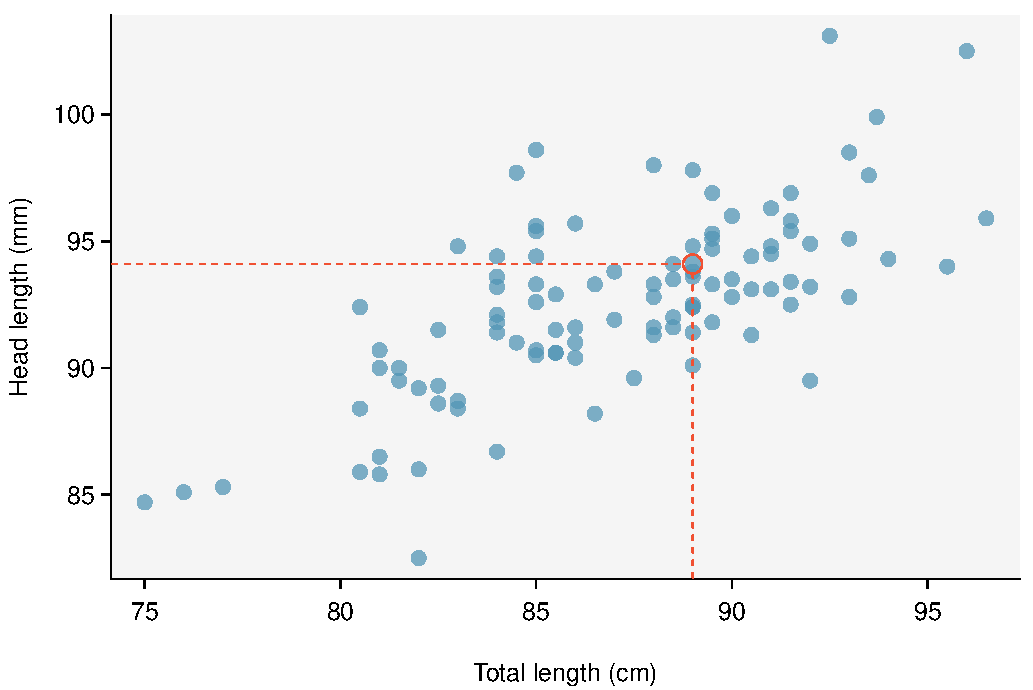
\includegraphics[width=0.8\textwidth]{ch_regr_simple_linear/figures/scattHeadLTotalL/scattHeadLTotalL}

   \caption{A scatterplot showing head length against total length for 104 brushtail possums. A point representing a possum with head length 94.1~mm and total length 89~cm is highlighted.}
   \label{scattHeadLTotalL}
\end{figure}

\D{\newpage}

The head and total length variables are associated: possums with an above average total length also tend to have above average head lengths. While the relationship is not perfectly linear, it could be helpful to partially explain the connection between these variables with a straight line.


%Straight lines should only be used when the data appear to have a linear relationship, such as the case shown in the left panel of Figure~\ref{scattHeadLTotalLTube}. The right panel of Figure~\ref{scattHeadLTotalLTube} shows a case where a curved line would be more useful in understanding the relationship between the two variables.

%\begin{onebox}{Watch out for curved trends}
%{We only consider models based on straight lines in this chapter. If data show a nonlinear trend, like that in the right panel of Figure~\ref{scattHeadLTotalLTube}, more advanced techniques should be used.\vspace{0.7mm}}
%\end{onebox}


We want to describe the relationship between the head length and total length variables in the possum data set using a line. In this example, we will use the total length, $x$, to explain or predict a possum's head length, $y$. When we use $x$ to predict $y$, we usually call $x$ the \term{explanatory variable} or predictor variable, and we call $y$ the \term{response variable}.  We could fit the linear relationship by eye, as in Figure~\ref{scattHeadLTotalLLine}. The equation for this line is
\begin{eqnarray*}
\hat{y} = 41 + 0.59x
\label{headLLinModTotalL}
\end{eqnarray*}
A ``hat'' on $y$ is used to signify that this is a predicted value, not an observed value.  We can use this line to discuss properties of possums. For instance, the equation predicts a possum with a total length of 80~cm will have a head length of
\begin{align*}
\hat{y} &= 41 + 0.59(80) \\
	&= 88.2 % mm
\end{align*}
The value $\hat{y}$ may be viewed as an average: the equation predicts that possums with a total length of 80~cm will have an average head length of 88.2~mm. The value $\hat{y}$ is also a prediction:  absent further information about an 80~cm possum, this is our best prediction for a the head length of a single 80~cm possum.  


\D{\newpage}

%%
\subsection{Residuals}

\index{residual|(}

\termsub{Residuals}{residual} are the leftover variation in the response variable after fitting a model.  Each observation will have a residual, and three of the residuals for the linear model we fit for the \data{possum} data are shown in Figure~\ref{scattHeadLTotalLLine}.  If an observation is above the regression line, then its residual, the vertical distance from the observation to the line, is positive.  Observations below the line have negative residuals.  One goal in picking the right linear model is for these residuals to be as small as possible.

\begin{figure}[h]
   \centering
   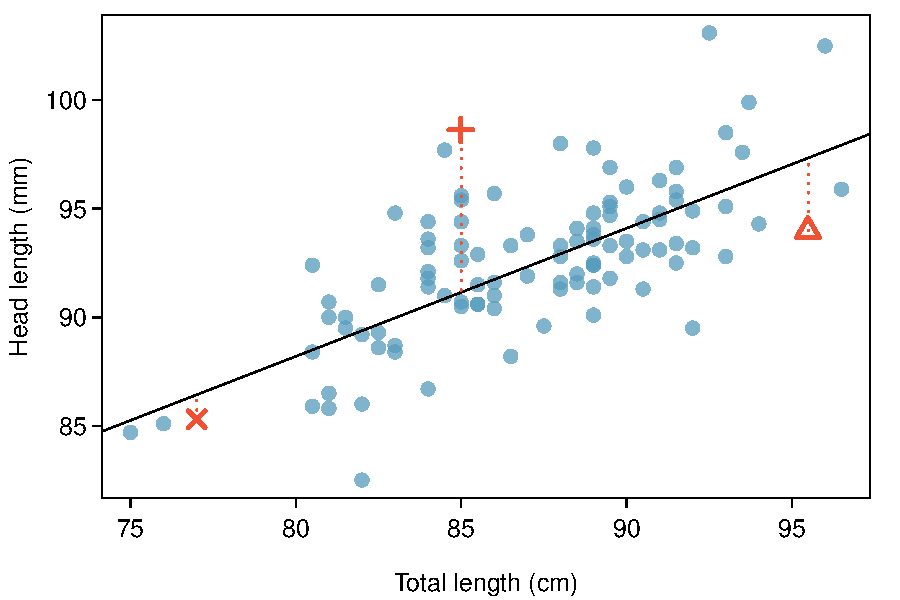
\includegraphics[width=0.7\textwidth]{ch_regr_simple_linear/figures/scattHeadLTotalLLine/scattHeadLTotalLLine}
   \caption{A reasonable linear model was fit to represent the relationship between head length and total length.}
   \label{scattHeadLTotalLLine}
\end{figure}

Let's look closer at the three residuals featured in Figure~\ref{scattHeadLTotalLLine}.  The observation marked by an ``$\times$'' has a small, negative residual of about -1; the observation marked by ``$+$'' has a large residual of about +7; and the observation marked by ``$\triangle$'' has a moderate residual of about -4. The size of a residual is usually discussed in terms of its absolute value. For example, the residual for ``$\triangle$'' is larger than that of ``$\times$'' because $|-4|$ is larger than $|-1|$.

%\Comment{remove use of $e_i$ since students don't need that}



\begin{onebox}{Residual: difference between observed and expected}
The residual for a particular observation $(x, \ y)$ is the difference between the observed response and the response we would predict based on the model:
\begin{align*}
\text{residual} =& \ \text{observed } y - \text{predicted } y\\
 =&\  y - \hat{y}
\end{align*}
We typically identify $\hat{y}$ by plugging $x$ into the model.\end{onebox}

\begin{examplewrap}
\begin{nexample}{The linear fit shown in Figure~\ref{scattHeadLTotalLLine} is given as $\hat{y} = 41 + 0.59x$. Based on this line, compute and interpret the residual of the observation $(77.0, \ 85.3)$. This observation is denoted by ``$\times$'' on the plot. Recall that $x$ is the total length measured in~cm and $y$ is head length measured in~mm.}
We first compute the predicted value based on the model:
\begin{align*}
\hat{y} =& \ 41+0.59x \\
=& \ 41+0.59(77.0)\\
=& \  86.4
\end{align*}
Next we compute the difference of the actual head length and the predicted head length:
\begin{align*}
residual =& \ y - \hat{y} \\
=& \ 85.3 -  86.4 \\
=& \ -1.1
\end{align*}
The residual for this point is -1.1~mm, which is very close to the visual estimate of -1~mm.  For this particular possum with total length of 77~cm, the model's prediction for its head length was 1.1~mm \emph{too high}.
\end{nexample}
\end{examplewrap}


\begin{exercisewrap}
\begin{nexercise}
If a model underestimates an observation, will the residual be positive or negative? What about if it overestimates the observation?\footnotemark 
\end{nexercise}
\end{exercisewrap}
\footnotetext{If a model underestimates an observation, then the model estimate is below the actual. The residual, which is the actual observation value minus the model estimate, must then be positive. The opposite is true when the model overestimates the observation: the residual is negative.}

\begin{exercisewrap}
\begin{nexercise}
Compute the residual for the observation $(95.5, 94.0)$, denoted by ``$\triangle$'' in the figure, using the linear model: $\hat{y} = 41 + 0.59x$.\footnotemark 
\end{nexercise}
\end{exercisewrap}
\footnotetext{First compute the predicted value based on the model, then compute the residual.
$$\hat{y} = 41+0.59x = 41 + 0.59(95.50) = 97.3$$
$$residual = y - \hat{y} = 94.0 - 97.3 = -3.3$$
The residual is -3.3, so the model \emph{overpredicted} the head length for this possum by 3.3~mm.}

Residuals are helpful in evaluating how well a linear model fits a data set. We often display the residuals in a \term{residual plot} such as the one shown in Figure~\ref{scattHeadLTotalLResidualPlotReproduced}.  Here, the residuals are calculated for each $x$ value, and plotted versus $x$.  For instance, the point $(85.0,98.6)$ had a residual of 7.45, so in the residual plot it is placed at $(85.0, 7.45)$. Creating a residual plot is sort of like tipping the scatterplot over so the regression line is horizontal. 

From the residual plot, we can better estimate the \term{standard deviation of the residuals}, often denoted by the letter $s$. The standard deviation of the residuals tells us  typical size of the residuals.  As such, it is a measure of the typical deviation between the $y$ values and the model predictions.  In other words, it tells us the typical prediction error using the model.\footnote{The standard deviation of the residuals is calculated as:  $s=\sqrt{\frac{\sum{(y_i-\hat{y})^2}}{n-2}}$. }

\D{\newpage}

\begin{examplewrap}
\begin{nexample}{Estimate the standard deviation of the residuals for predicting head length from total length using the line: $\hat{y} = 41+0.59x$ using
Figure~\ref{scattHeadLTotalLResidualPlotReproduced}.
Also, interpret the quantity in context.}
To estimate this graphically, we use the residual plot.  The approximate 68, 95 rule for standard deviations applies.  Approximately 2/3 of the points are within $\pm$ 2.5 and approximately 95\% of the points are within $\pm$ 5, so 2.5 is a good estimate for the standard deviation of the residuals.  The typical error when predicting head length using this model is about 2.5~mm.
\end{nexample}
\end{examplewrap}

\index{data!possum|)}

\begin{figure}[h]
   \centering
  \begin{tabular}{cc}
   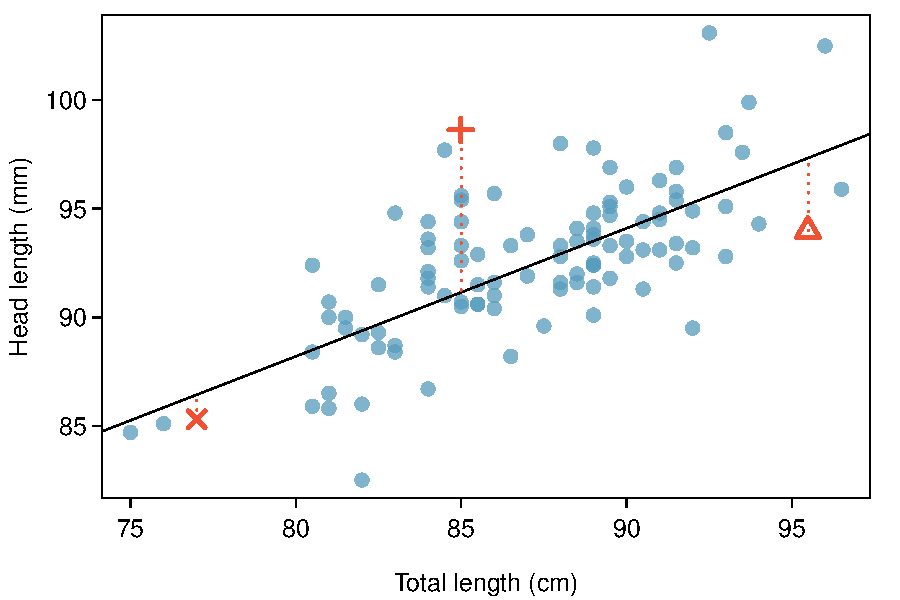
\includegraphics[width=0.5\textwidth]{ch_regr_simple_linear/figures/scattHeadLTotalLLine/scattHeadLTotalLLine}%
   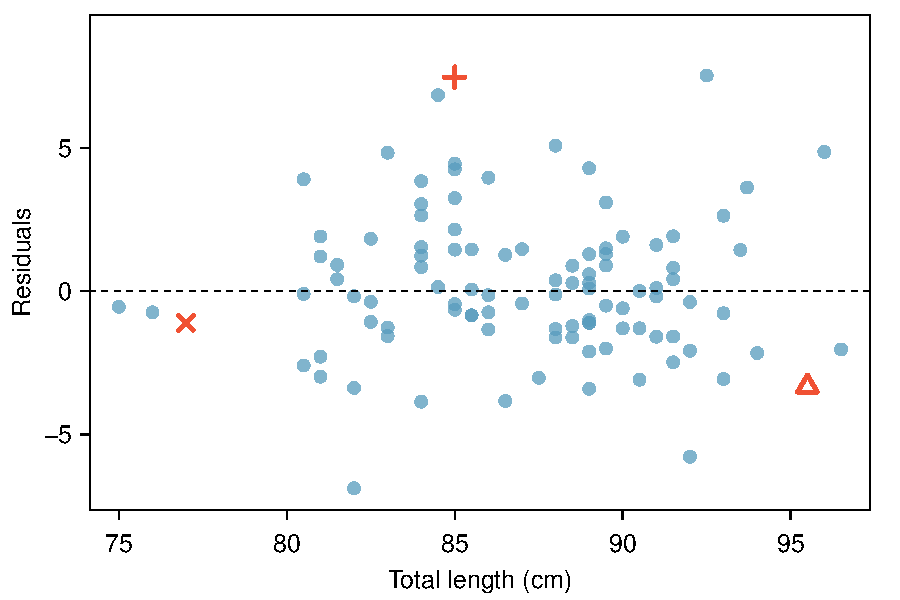
\includegraphics[width=0.5\textwidth]{ch_regr_simple_linear/figures/scattHeadLTotalLResidualPlot/scattHeadLTotalLResidualPlot}
\end{tabular}
   \caption{Left: Scatterplot of head length versus total length for 104 brushtail possums.  Three particular points have been highlighted.  Right: Residual plot for the model shown in left panel.  }
   \label{scattHeadLTotalLResidualPlotReproduced}
\end{figure}

\begin{onebox}{Standard deviation of the residuals}
The standard deviation of the residuals, often denoted by the letter $s$, tells us the typical error in the predictions using the regression model.  It can be estimated from a residual plot.
\end{onebox}

\D{\newpage}

\begin{examplewrap}
\begin{nexample}{One purpose of residual plots is to identify characteristics or patterns still apparent in data after fitting a model. Figure~\ref{sampleLinesAndResPlots} shows three scatterplots with linear models in the first row and residual plots in the second row. Can you identify any patterns remaining in the residuals?}


In the first data set (first column), the residuals show no obvious patterns. The residuals appear to be scattered randomly around the dashed line that represents 0.

The second data set shows a pattern in the residuals. There is some curvature in the scatterplot, which is more obvious in the residual plot. We should not use a straight line to model these data. Instead, a more advanced technique should be used.

The last plot shows very little upwards trend, and the residuals also show no obvious patterns. It is reasonable to try to fit a linear model to the data. However, it is unclear whether there is statistically significant evidence that the slope parameter is different from zero. The slope of the sample regression line is not zero, but we might wonder if this could be due to random variation. We will address this sort of scenario in Section~\ref{inferenceForLinearRegression}.
\index{residual|)}
\end{nexample}
\end{examplewrap}

\begin{figure}[h]
   \centering
   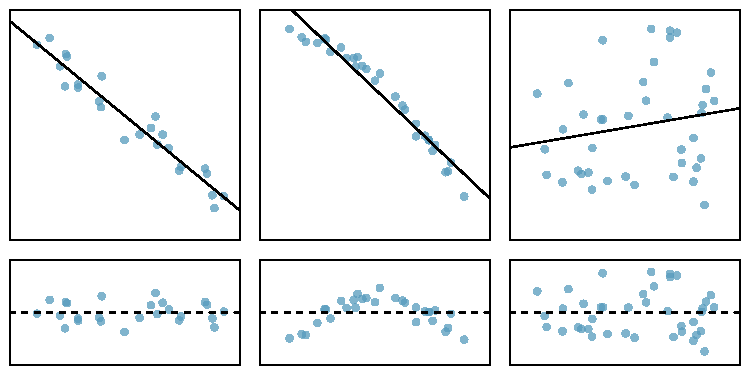
\includegraphics[width=\textwidth]{ch_regr_simple_linear/figures/sampleLinesAndResPlots/sampleLinesAndResPlots}
   \caption{Sample data with their best fitting lines (top row) and their corresponding residual plots (bottom row).}
   \label{sampleLinesAndResPlots}
\end{figure}


\D{\newpage}

%%
\subsection{Describing linear relationships with correlation}

\index{correlation|(}

When a linear relationship exists between two variables, we can quantify the strength and direction of the linear relation with the correlation coefficient, or just \term{correlation} for short.  Figure~\ref{posNegCorPlots} shows eight plots and their corresponding correlations. 

\begin{figure}[h]
   \centering
   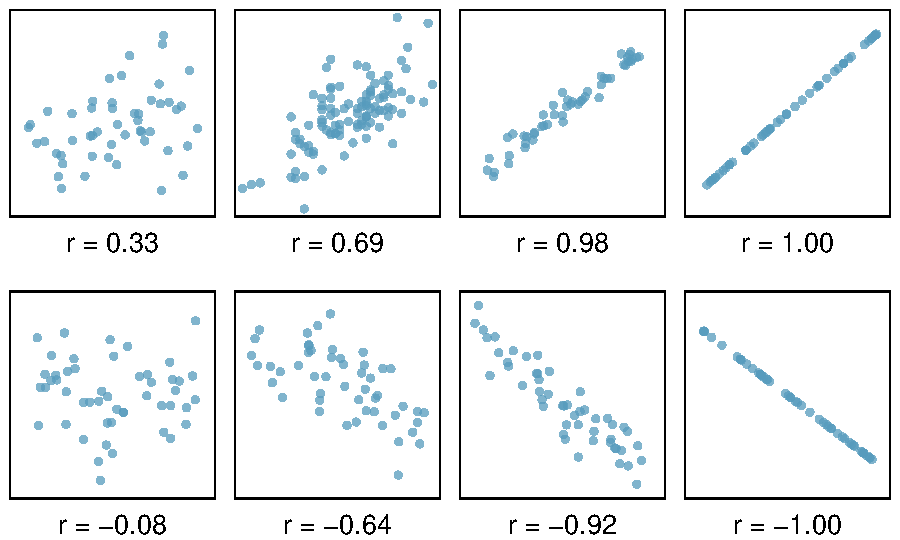
\includegraphics[width=0.8\textwidth]{ch_regr_simple_linear/figures/posNegCorPlots/posNegCorPlots}
   \caption{Sample scatterplots and their correlations. The first row shows variables with a positive relationship, represented by the trend up and to the right. The second row shows variables with a negative trend, where a large value in one variable is associated with a low value in the other.}
   \label{posNegCorPlots}
\end{figure}

Only when the relationship is perfectly linear is the correlation either $-1$ or 1. If~the linear relationship is strong and positive, the correlation will be near +1. If it is strong and negative, it will be near $-1$. If~there is no apparent linear relationship between the variables, then the correlation will be near zero.


\begin{onebox}{Correlation measures the strength of a linear relationship}
\termsub{Correlation}{correlation}, which always takes values between -1 and 1, describes the direction and strength of the linear relationship between two numerical variables. The strength can be strong, moderate, or~weak.\end{onebox}


We compute the correlation using a formula, just as we did with the sample mean and standard deviation. Formally, we can compute the correlation for observations $(x_1, y_1)$, $(x_2, y_2)$, ..., $(x_n, y_n)$ using the formula
\begin{align*}
r =\frac{1}{n-1}\sum{\Big(\frac{x_i-\bar{x}}{s_x}\Big)\Big(\frac{y_i-\bar{y}}{s_y}\Big)}
\end{align*} 
where $\bar{x}$, $\bar{y}$, $s_x$, and $s_y$ are the sample means and standard deviations for each variable.  This formula is rather complex, and we generally perform the calculations on a computer or calculator. We can note, though, that the computation involves taking, for each point, the product of the Z-scores that correspond to the $x$ and $y$ values. 


\begin{examplewrap}
\begin{nexample}
{Take a look at Figure~\ref{scattHeadLTotalLLine} on page~\pageref{scattHeadLTotalLLine}.  How would the correlation between head length and total body length of possums change if head length were measured in~cm rather than~mm?  What if head length were measured in inches rather than~mm?}Here, changing the units of $y$ corresponds to multiplying all the $y$ values by a certain number.  This would change the mean and the standard deviation of $y$, but it would not change the correlation.  To see this, imagine dividing every number on the vertical axis by 10.  The units of $y$ are now in~cm rather than in~mm, but the graph has remain exactly the same.  The units of $y$ have changed, by the relative distance of the $y$ values about the mean are the same; that is, the Z-scores corresponding to the $y$~values have remained the same.
\end{nexample}
\end{examplewrap}

\begin{onebox}{Changing units of \pmb{$x$} and \pmb{$y$} does not affect the correlation}
The correlation, $r$, between two variables is not dependent upon the units in which the variables are recorded.  Correlation itself has no units. \end{onebox}



Correlation is intended to quantify the strength of a linear trend. Nonlinear trends, even when strong, sometimes produce correlations that do not reflect the strength of the relationship; see three such examples in Figure~\ref{corForNonLinearPlots}.

\begin{figure}[h]
   \centering
   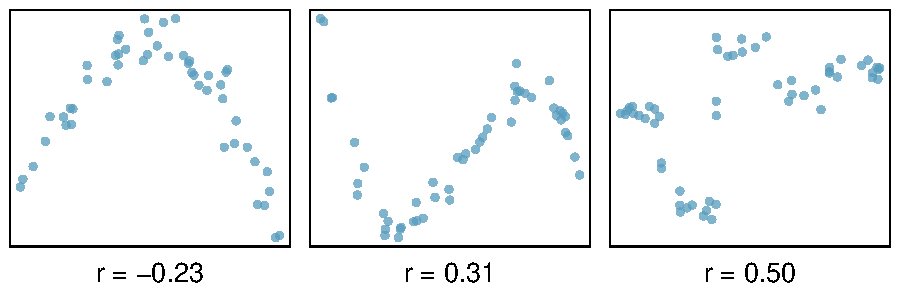
\includegraphics[width=0.96\textwidth]{ch_regr_simple_linear/figures/posNegCorPlots/corForNonLinearPlots}
   \caption{Sample scatterplots and their correlations. In each case, there is a strong relationship between the variables. However, the correlation is not very strong, and the relationship is not linear.}
   \label{corForNonLinearPlots}
\end{figure}

\begin{exercisewrap}
\begin{nexercise}
It appears no straight line would fit any of the datasets represented in Figure~\ref{corForNonLinearPlots}. Try drawing nonlinear curves on each plot. Once you create a curve for each, describe what is important in your fit.\footnotemark 
\index{correlation|)}
\end{nexercise}
\end{exercisewrap}
\footnotetext{We'll leave it to you to draw the lines. In general, the lines you draw should be close to most points and reflect overall trends in the data.}
%%

\D{\newpage}
 
\begin{examplewrap}
\begin{nexample}{Consider the four scatterplots in Figure~\ref{anscombe}.  In which scatterplot is the correlation between $x$ and $y$ the strongest?}
All four data sets have the exact same correlation of $r = 0.816$ as well as the same equation for the best fit line!  This group of four graphs, known as Anscombe's Quartet, remind us that knowing the value of the correlation does not tell us what the corresponding scatterplot looks like.  It is always important to first graph the data.  Investigate Anscombe's Quartet in Desmos: \oiRedirect{desmos-anscombe}{\small{https://www.desmos.com/calculator/paknt6oneh}}.
\end{nexample}
\end{examplewrap}

\begin{figure}[h]
   \centering
\oiRedirect{desmos-anscombe}{
   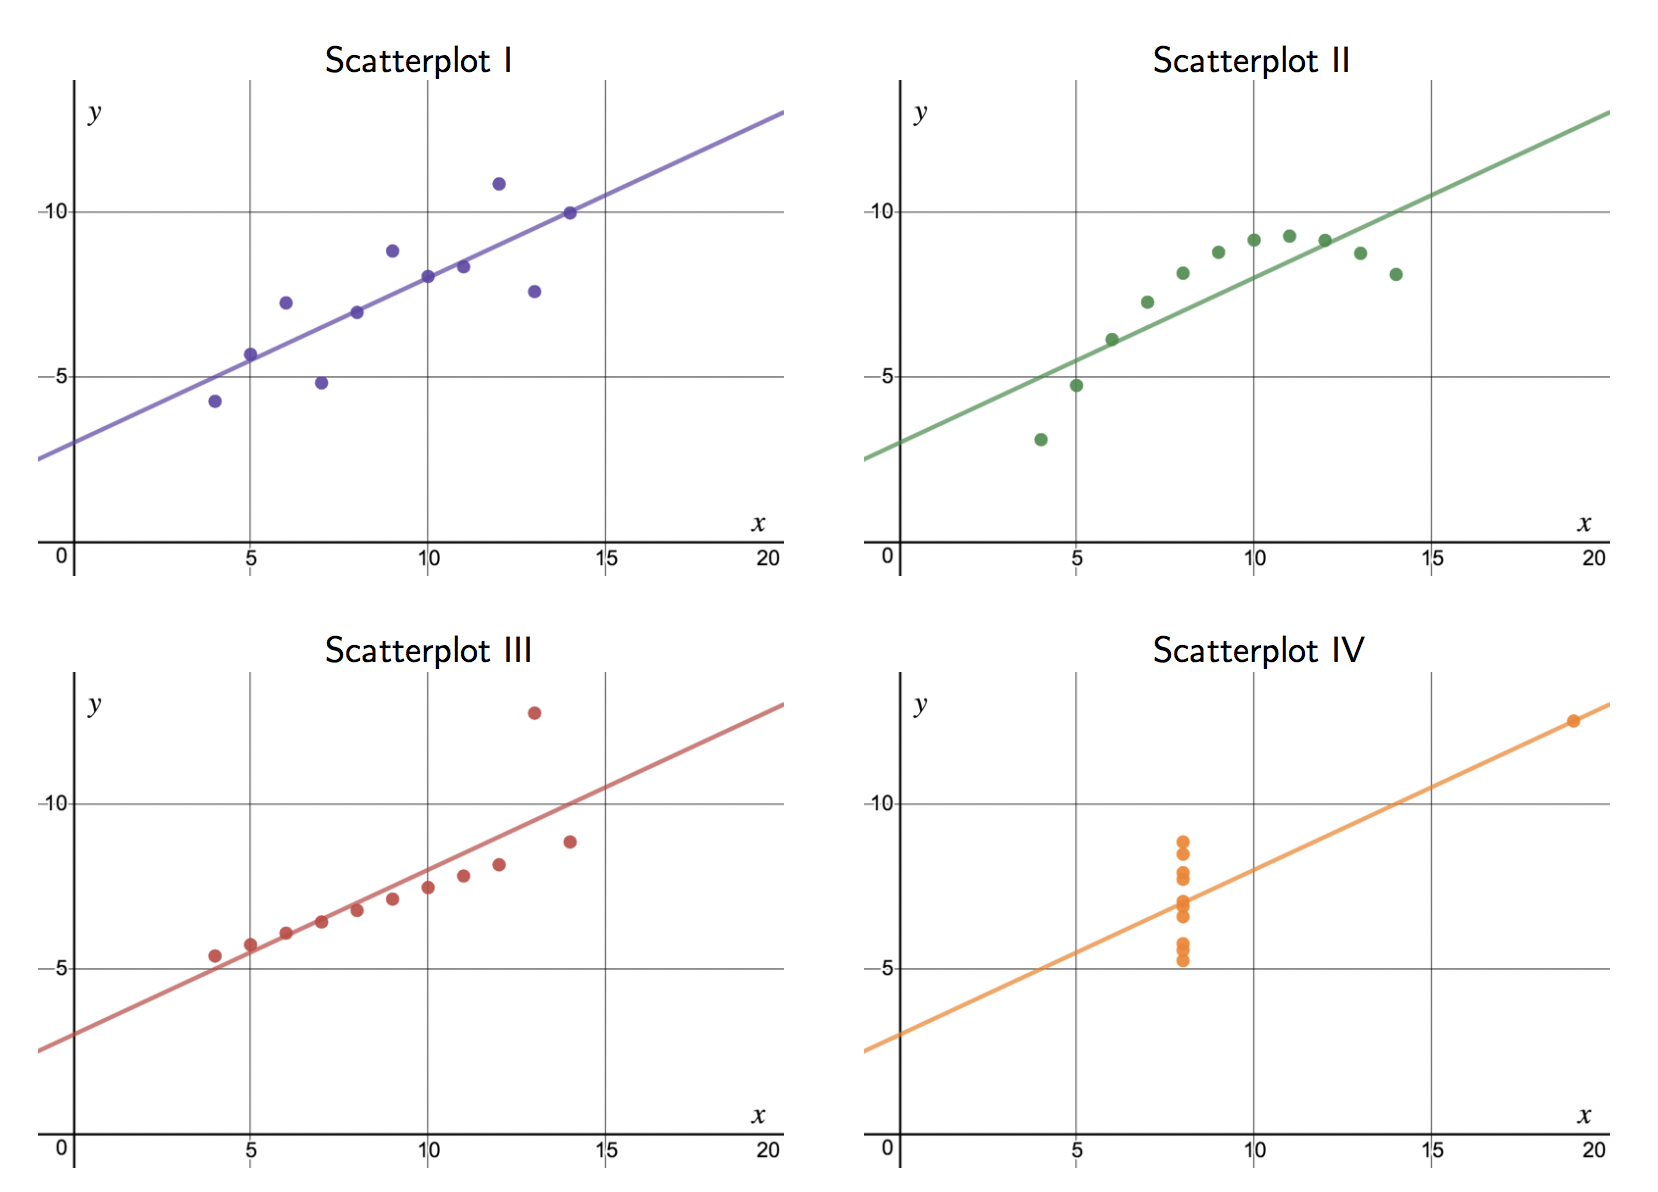
\includegraphics[width=\textwidth]{ch_regr_simple_linear/figures/anscombe/anscombeDesmos}}
   \caption{Four scatterplots from Desmos with best fit line drawn in.}
   \label{anscombe}
\end{figure}



\D{\newpage}

%%
\subsection*{Section summary}
\begin{itemize}

\item In Chapter 2 we introduced a bivariate display called a \termsub{scatterplot}{scatterplot}, which shows the relationship between two numerical variables.  When we use $x$ to predict $y$, we call $x$ the \term{explanatory variable} or predictor variable, and we call $y$ the \term{response variable}.

\item A linear model for bivariate numerical data can be useful for prediction when the association between the variables follows a constant, linear trend.  Linear models should not be used if the trend between the variables is curved.  

\item When we write a linear model, we use $\hat{y}$ to indicate that it is the model or the prediction.   The value $\hat{y}$ can be understood as a \term{prediction} for $y$ based on a given $x$, or as an \term{average} of the $y$ values for a given $x$.

\item The \term{residual} is the \textbf{error} between the true value and the modeled value, computed as $y - \hat{y}$.  The order of the difference matters, and the sign of the residual will tell us if the model overpredicted or underpredicted a particular data point.

\item The symbol $s$ in a linear model is used to denote the standard deviation of the residuals, and it measures the typical prediction error by the model.

\item A \term{residual plot} is a scatterplot with the residuals on the vertical axis.  The residuals are often plotted against $x$ on the horizontal axis, but they can also be plotted against $y$, $\hat{y}$, or other variables.  Two important uses of a residual plot are the following.
\begin{itemize}
\item Residual plots help us see patterns in the data that may not have been apparent in the scatterplot.
\item The standard deviation of the residuals is easier to estimate from a residual plot than from the original scatterplot.
\end{itemize}

\item \termsub{Correlation}{correlation}, denoted with the letter $r$, measures the strength and direction of a linear relationship.  The following are some important facts about correlation.
\begin{itemize}
\item The value of $r$ is always between $-1$ and $1$, inclusive, with an $r=-1$ indicating a perfect negative relationship (points fall exactly along a line that has negative slope) and an $r=1$ indicating a perfect positive relationship (points fall exactly along a line that has positive slope).  
\item An $r=0$ indicates no \emph{linear} association between the variables, though there may well exist a quadratic or other type of association.
\item Just like Z-scores, the correlation has no units.  Changing the units in which $x$ or $y$ are measured does not affect the correlation.
\item Correlation is sensitive to outliers.  Adding or removing a single point can have a big effect on the correlation.
\item As we learned previously, correlation is not causation.  Even a very strong correlation cannot prove causation; only a well-designed, controlled, randomized experiment can prove causation.  \end{itemize}


\end{itemize}




%%%%%%%%Section Exercises
{\exercisesheader{}

% 1

\eoce{\qt{Visualize the residuals\label{visualize_residuals}} 
The scatterplots shown below each have a 
superimposed regression line. If we were to construct a residual plot 
(residuals versus $x$) for each, describe what those plots would look 
like.
\begin{center}
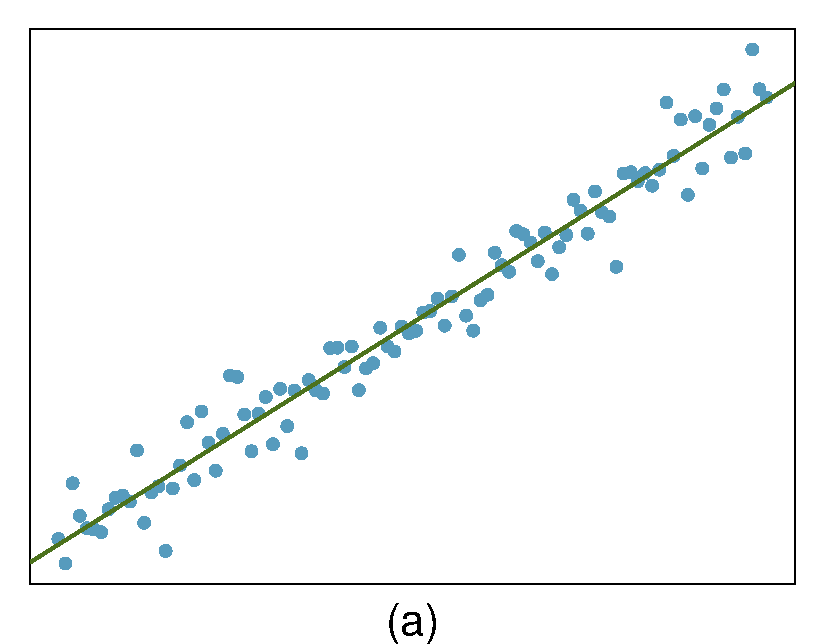
\includegraphics[width=0.42\textwidth]{ch_regr_simple_linear/figures/eoce/visualize_residuals/visualize_residuals_linear.pdf} 
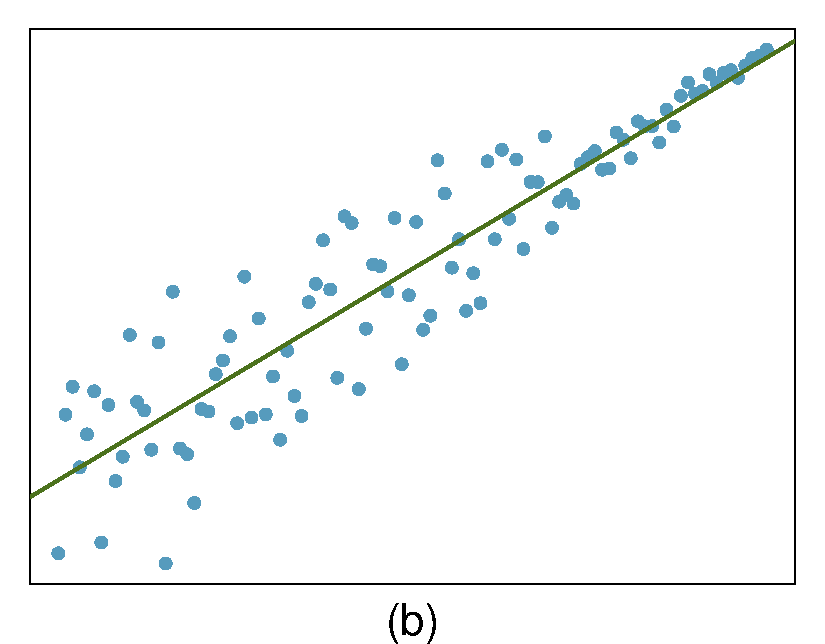
\includegraphics[width=0.42\textwidth]{ch_regr_simple_linear/figures/eoce/visualize_residuals/visualize_residuals_fan_back.pdf}
\end{center}
}{}

% 2

\eoce{\qt{Trends in the residuals\label{trends_in_residuals}} 
Shown below are two plots of residuals 
remaining after fitting a linear model to two different sets of data. 
Describe important features and determine if a linear model would be 
appropriate for these data. Explain your reasoning.
\begin{center}
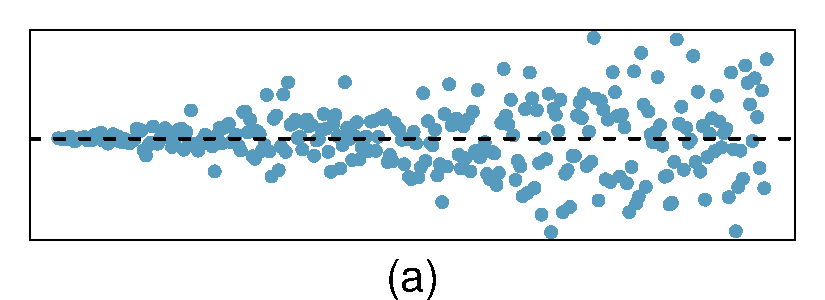
\includegraphics[width=0.42\textwidth]{ch_regr_simple_linear/figures/eoce/trends_in_residuals/trends_in_residuals_fan.pdf} 
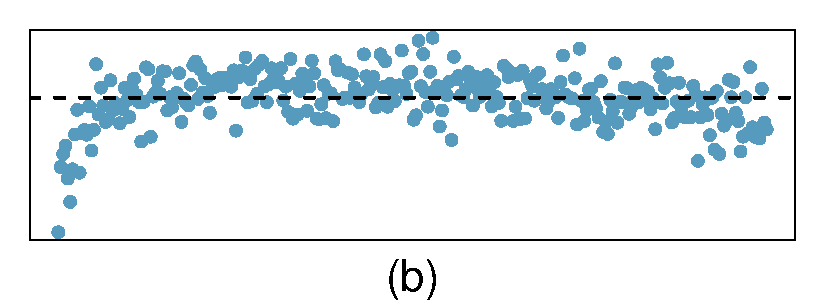
\includegraphics[width=0.42\textwidth]{ch_regr_simple_linear/figures/eoce/trends_in_residuals/trends_in_residuals_log.pdf}
\end{center}
}{}

% 3

\eoce{\qt{Identify relationships, Part I\label{identify_relationships_1}} 
For each of the six plots, 
identify the strength of the relationship (e.g. weak, moderate, or 
strong) in the data and whether fitting a linear model would be 
reasonable.
\begin{center}
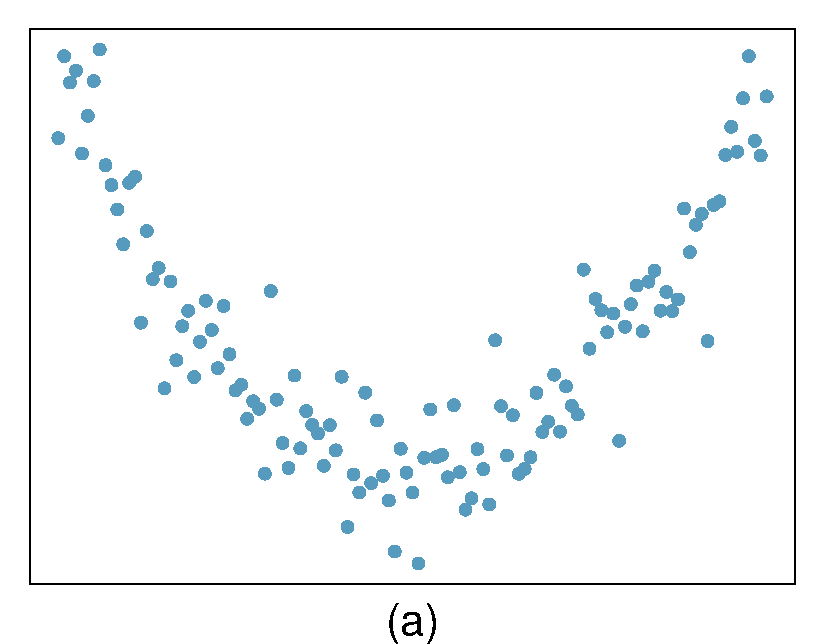
\includegraphics[width=0.32\textwidth]{ch_regr_simple_linear/figures/eoce/identify_relationships_1/identify_relationships_u.pdf}
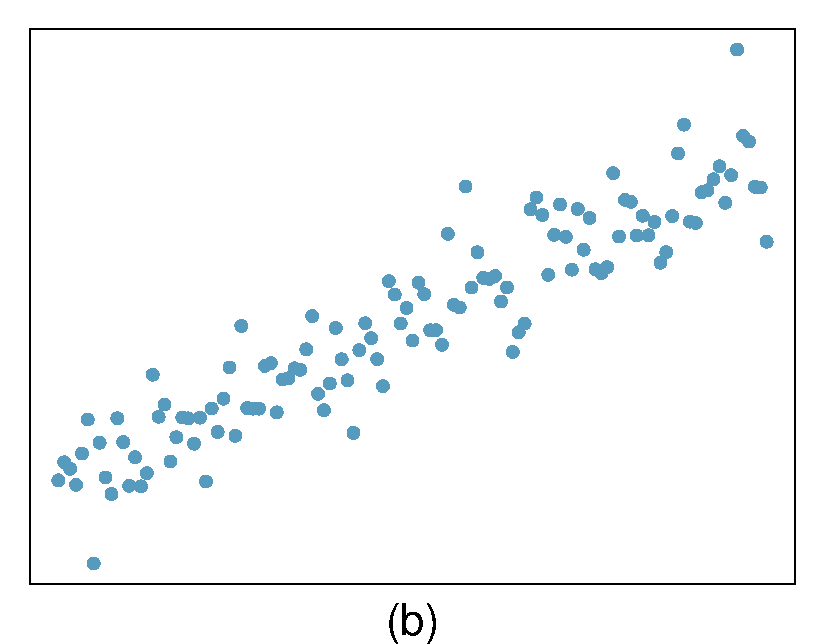
\includegraphics[width=0.32\textwidth]{ch_regr_simple_linear/figures/eoce/identify_relationships_1/identify_relationships_lin_pos_strong.pdf}
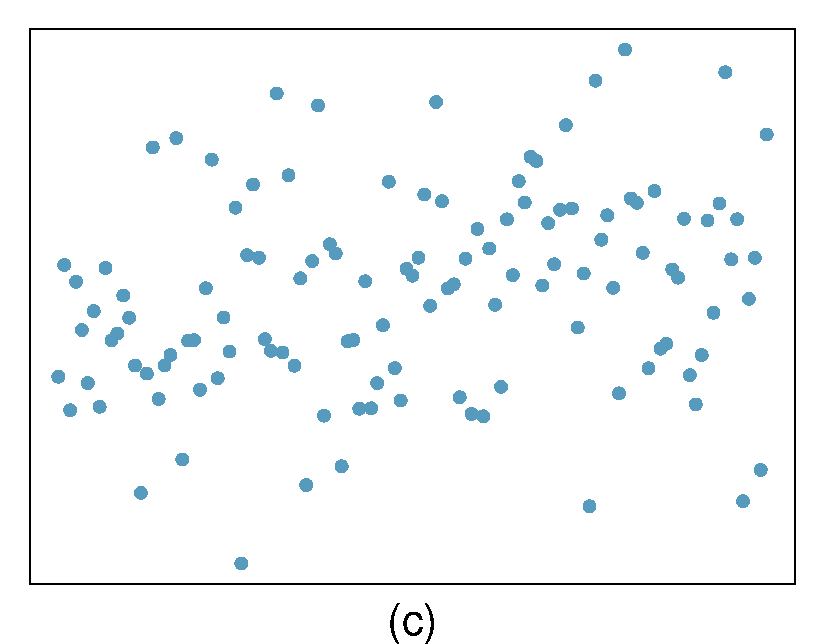
\includegraphics[width=0.32\textwidth]{ch_regr_simple_linear/figures/eoce/identify_relationships_1/identify_relationships_lin_pos_weak.pdf}
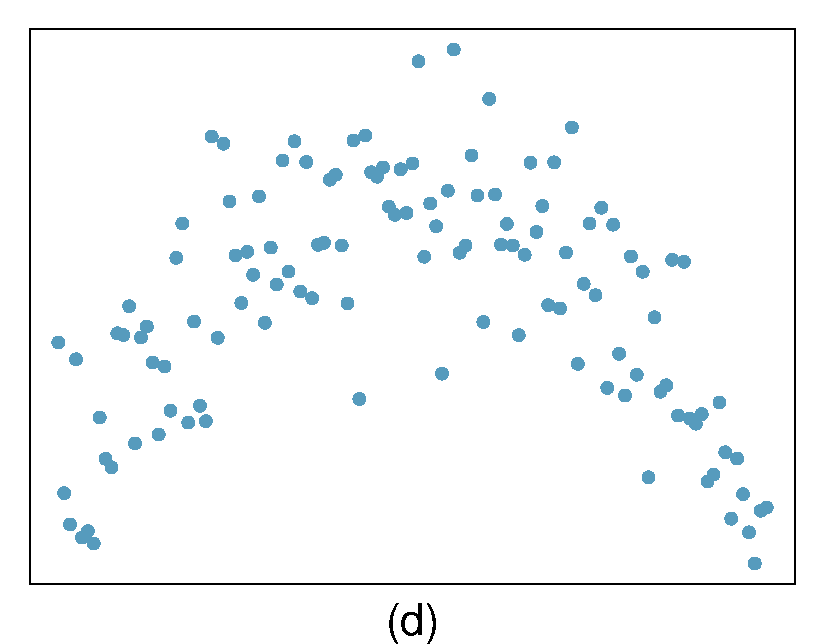
\includegraphics[width=0.32\textwidth]{ch_regr_simple_linear/figures/eoce/identify_relationships_1/identify_relationships_n.pdf}
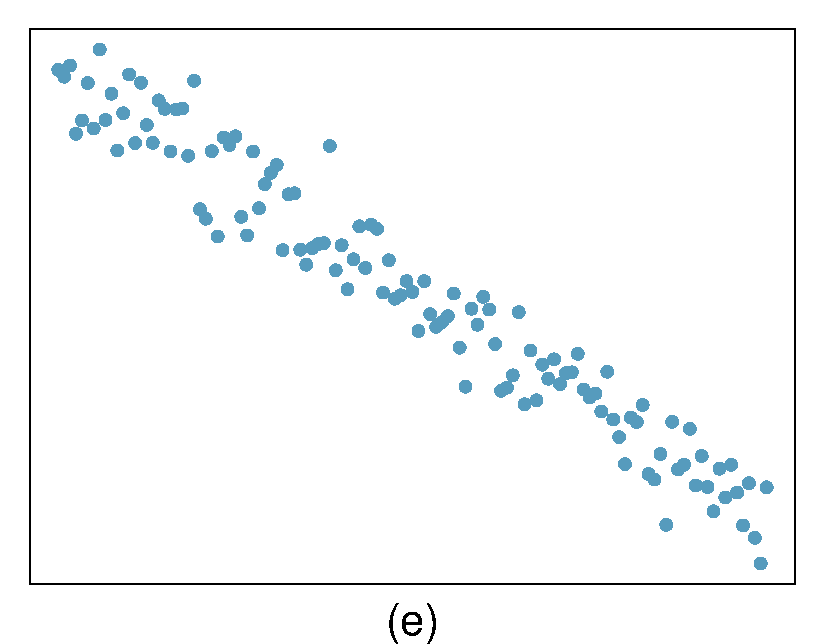
\includegraphics[width=0.32\textwidth]{ch_regr_simple_linear/figures/eoce/identify_relationships_1/identify_relationships_lin_neg_strong.pdf}
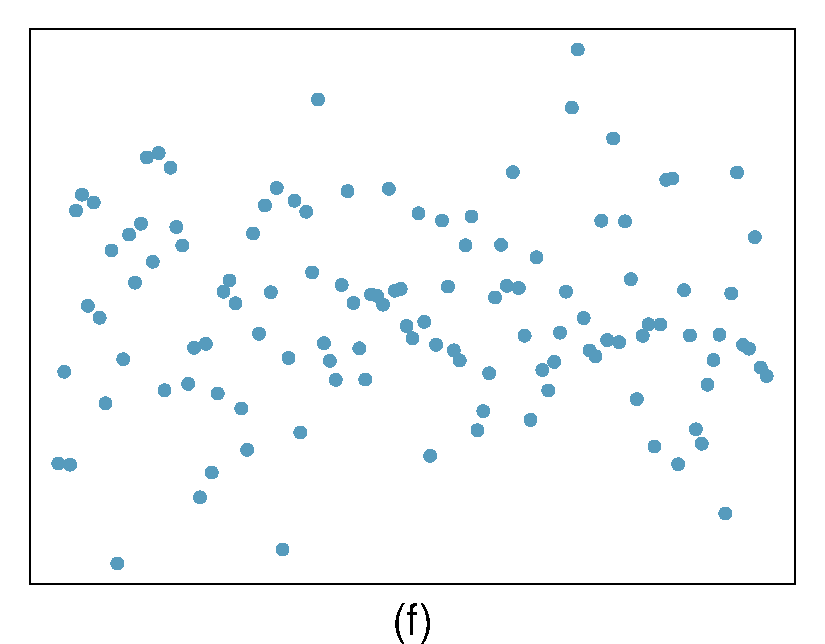
\includegraphics[width=0.32\textwidth]{ch_regr_simple_linear/figures/eoce/identify_relationships_1/identify_relationships_none.pdf}
\end{center}
}{}

\D{\newpage}
 
% 4

\eoce{\qt{Identify relationships, Part II\label{identify_relationships_2}} 
For each of the six plots, 
identify the strength of the relationship (e.g. weak, moderate, or 
strong) in the data and whether fitting a linear model would be 
reasonable.
\begin{center}
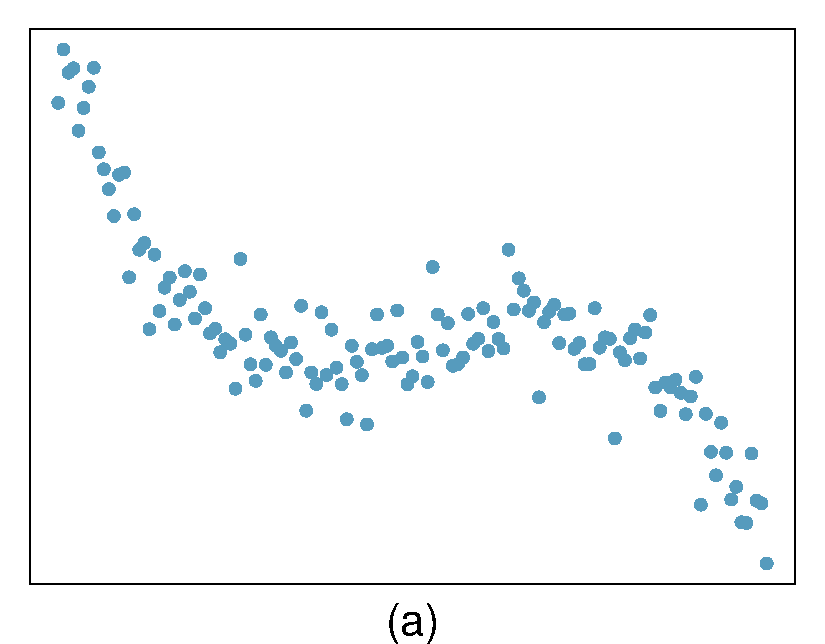
\includegraphics[width=0.32\textwidth]{ch_regr_simple_linear/figures/eoce/identify_relationships_2/identify_relationships_s.pdf}
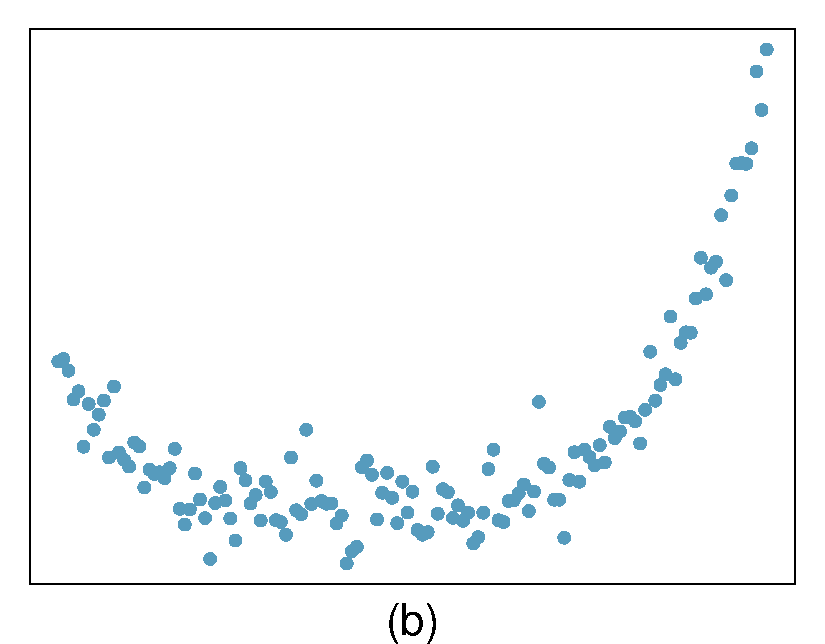
\includegraphics[width=0.32\textwidth]{ch_regr_simple_linear/figures/eoce/identify_relationships_2/identify_relationships_hockey_stick.pdf}
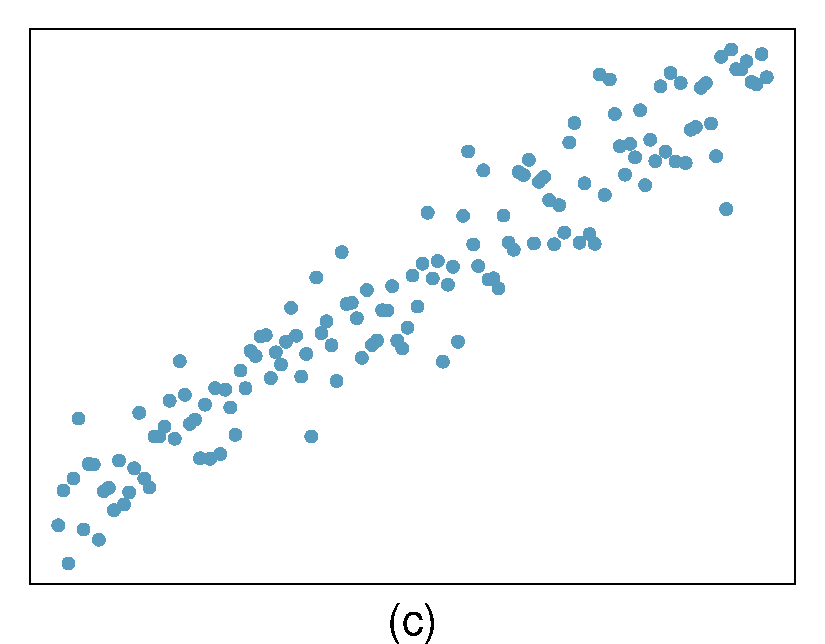
\includegraphics[width=0.32\textwidth]{ch_regr_simple_linear/figures/eoce/identify_relationships_2/identify_relationships_pos_lin_strong.pdf}
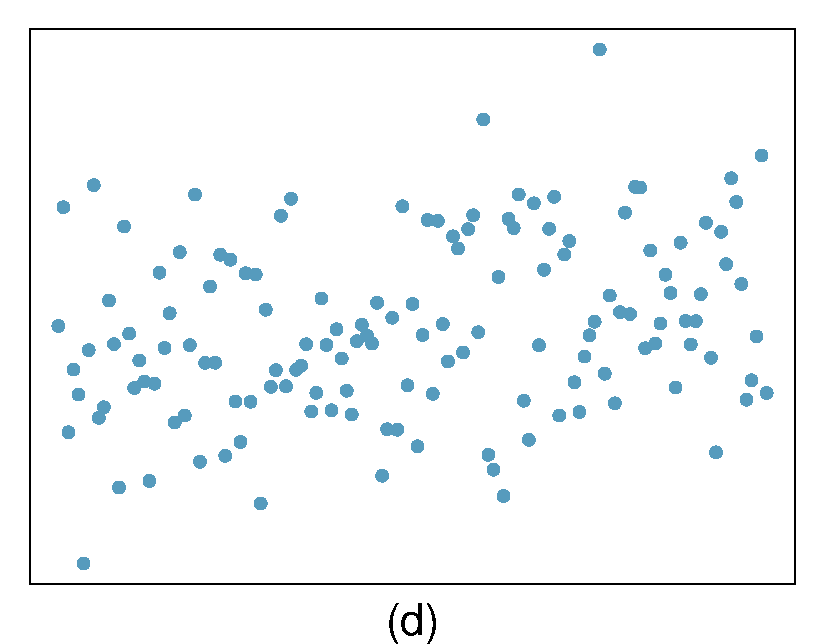
\includegraphics[width=0.32\textwidth]{ch_regr_simple_linear/figures/eoce/identify_relationships_2/identify_relationships_pos_weak.pdf}
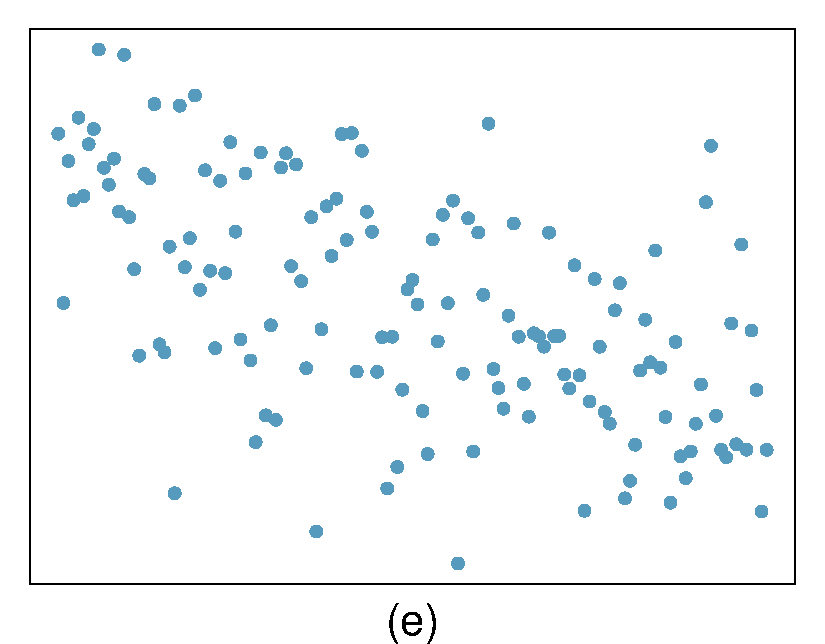
\includegraphics[width=0.32\textwidth]{ch_regr_simple_linear/figures/eoce/identify_relationships_2/identify_relationships_pos_weaker.pdf}
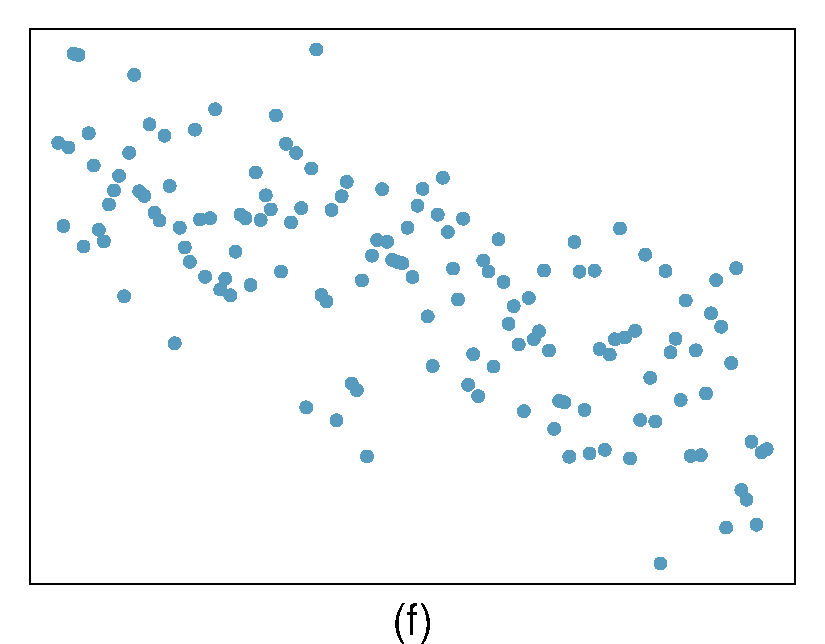
\includegraphics[width=0.32\textwidth]{ch_regr_simple_linear/figures/eoce/identify_relationships_2/identify_relationships_neg_lin_weak.pdf}
\end{center}
}{}

% 5

\eoce{\qt{Exams and grades\label{exams_grades_correlation}} 
The two scatterplots below show the 
relationship between final and mid-semester exam grades recorded 
during several years for a Statistics course at a university.
\begin{parts}
\item Based on these graphs, which of the two exams has the strongest 
correlation with the final exam grade? Explain.
\item Can you think of a reason why the correlation between the exam 
you chose in part (a) and the final exam is higher?
\end{parts}
\begin{center}
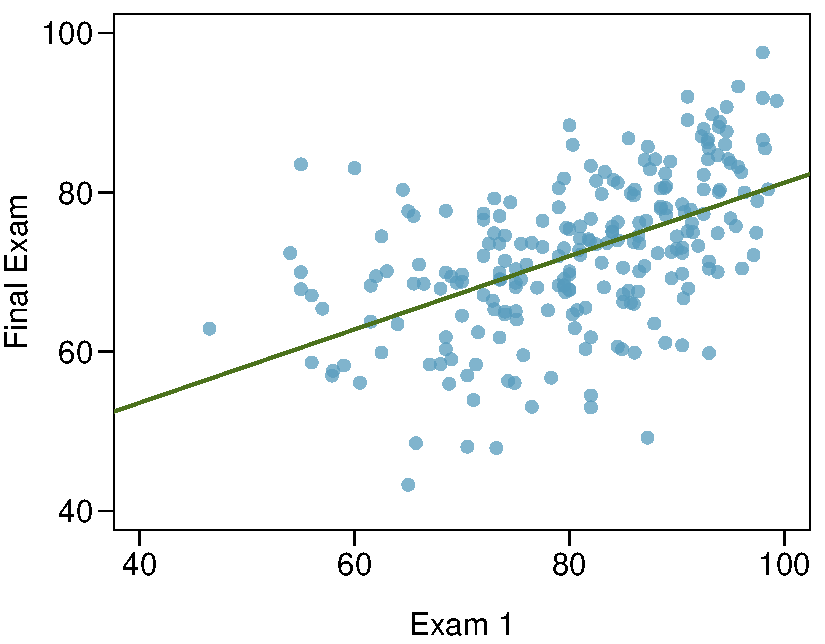
\includegraphics[width=0.485\textwidth]{ch_regr_simple_linear/figures/eoce/exams_grades_correlation/exam_grades_1.pdf}
\hspace{0.02\textwidth}%
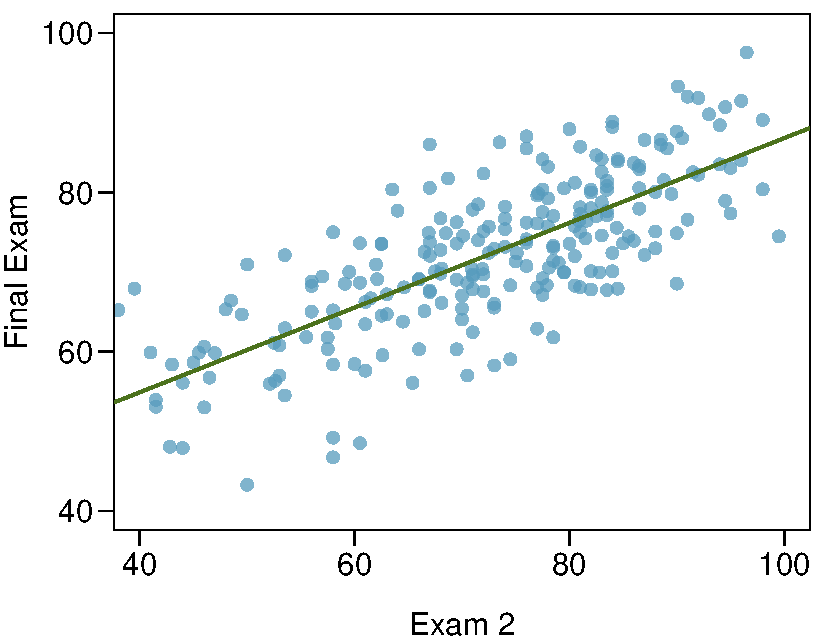
\includegraphics[width=0.485\textwidth]{ch_regr_simple_linear/figures/eoce/exams_grades_correlation/exam_grades_2.pdf}
\end{center}
}{}

\D{\newpage}
 
% 6

\eoce{\qt{Spouses, Part I\label{husbands_wives_correlation}}
The Great Britain Office of Population Census and Surveys once 
collected data on a random sample of 170 married women in 
Britain, recording the age (in years) and heights (converted 
here to inches) of the women and their spouses.\footfullcite{Hand:1994} 
The scatterplot on the left shows the spouse's age plotted against the woman's age, and the plot on the right shows spouse's height 
plotted against the woman's height.
\begin{center}
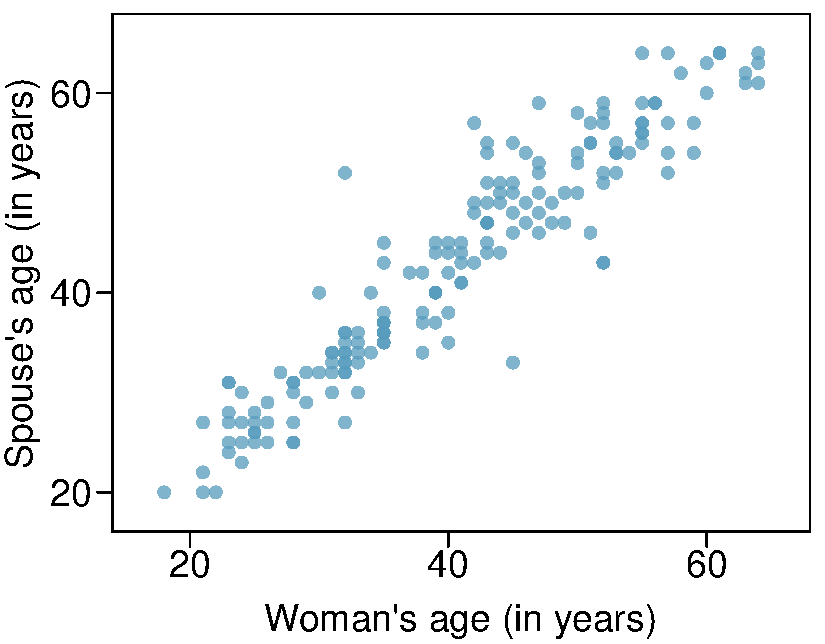
\includegraphics[width=0.36\textwidth]{ch_regr_simple_linear/figures/eoce/husbands_wives_correlation/husbands_wives_age.pdf} 
\hspace{5mm}
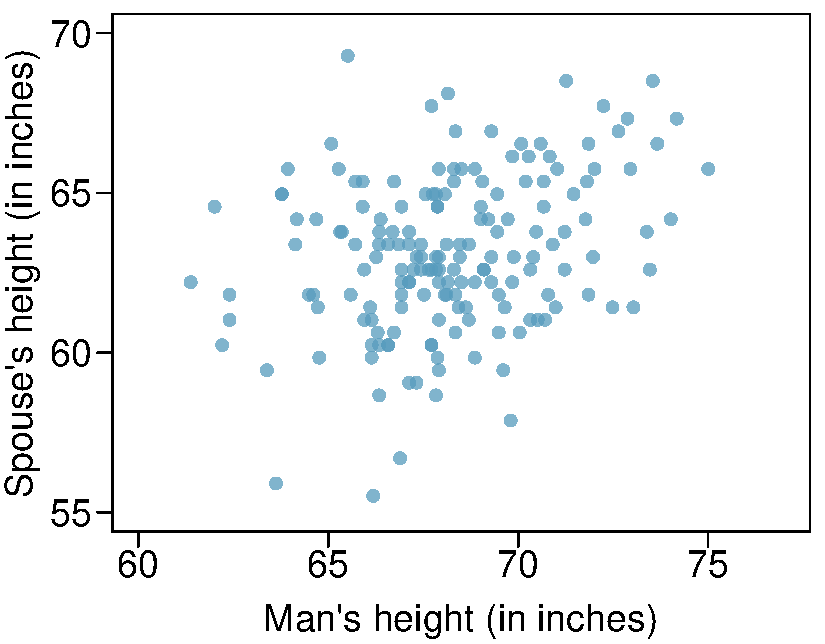
\includegraphics[width=0.36\textwidth]{ch_regr_simple_linear/figures/eoce/husbands_wives_correlation/husbands_wives_height.pdf}
\end{center}
\begin{parts}
\item Describe the relationship between the ages of women in the sample and their spouses' ages.
\item Describe the relationship between the heights of women in the sample and their spouses' heights.
\item Which plot shows a stronger correlation? Explain your reasoning.
\item Data on heights were originally collected in centimeters, and 
then converted to inches. Does this conversion affect the correlation 
between heights of women in the sample and their spouses' heights?
\end{parts}
}{}

% 7

\eoce{\qt{Match the correlation, Part I\label{match_corr_1}} 
Match each correlation to the corresponding scatterplot.

\noindent%
\begin{minipage}[c]{0.17\textwidth}
\begin{parts}
\item $r = -0.7$
\item $r = 0.45$ 
\item $r = 0.06$
\item $r = 0.92$
\end{parts}\vspace{3mm}
\end{minipage}%
\begin{minipage}[c]{0.83\textwidth}
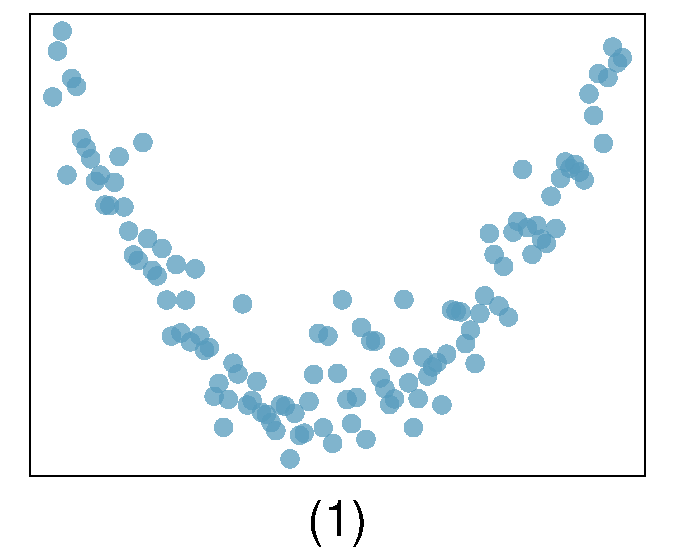
\includegraphics[width=0.225\textwidth]{ch_regr_simple_linear/figures/eoce/match_corr_1/match_corr_1_u}
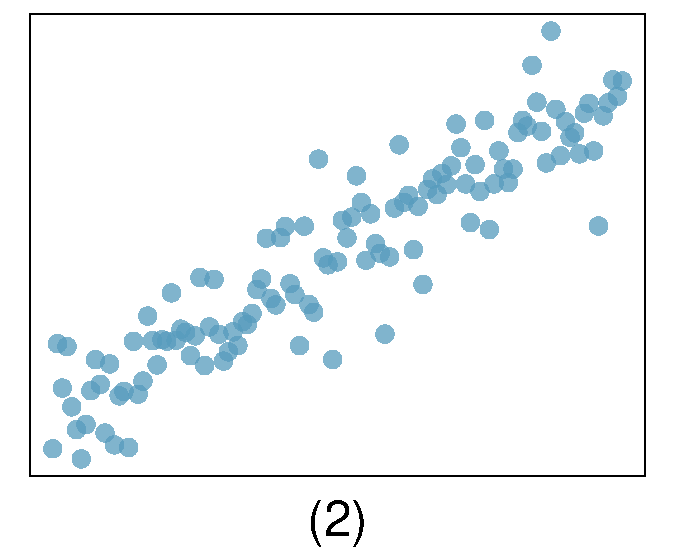
\includegraphics[width=0.225\textwidth]{ch_regr_simple_linear/figures/eoce/match_corr_1/match_corr_2_strong_pos}
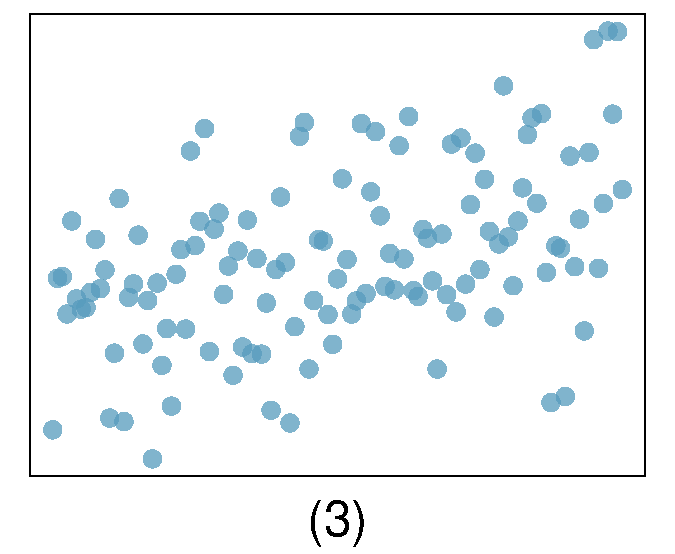
\includegraphics[width=0.225\textwidth]{ch_regr_simple_linear/figures/eoce/match_corr_1/match_corr_3_weak_pos}
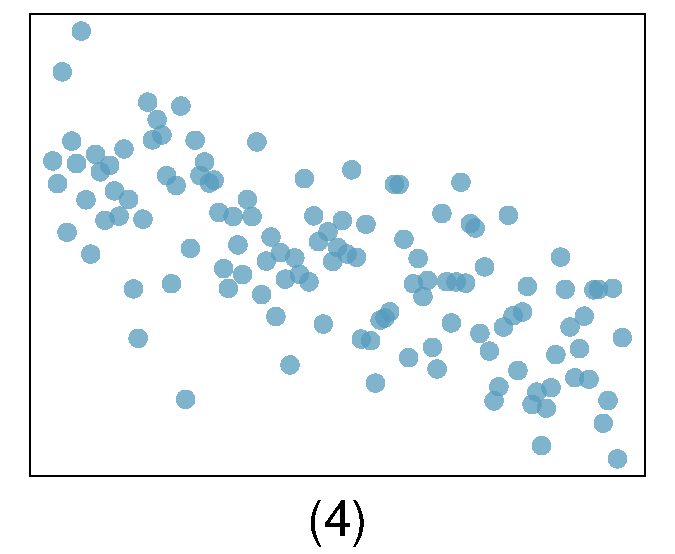
\includegraphics[width=0.225\textwidth]{ch_regr_simple_linear/figures/eoce/match_corr_1/match_corr_4_weak_neg}
\end{minipage}
}{}

% 8

\eoce{\qt{Match the correlation, Part II\label{match_corr_2}} 
Match each correlation to the corresponding scatterplot.

\noindent%
\begin{minipage}[c]{0.17\textwidth}
\begin{parts}
\item $r = 0.49$
\item $r = -0.48$ 
\item $r = -0.03$ 
\item $r = -0.85$
\end{parts}\vspace{3mm}
\end{minipage}%
\begin{minipage}[c]{0.83\textwidth}
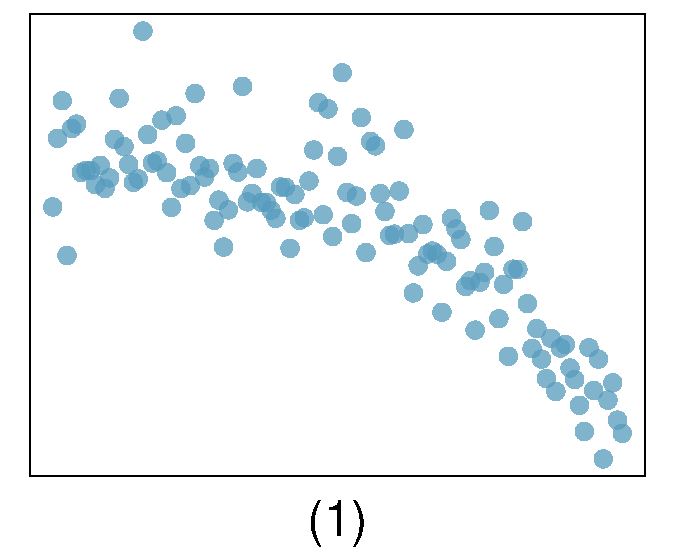
\includegraphics[width=0.245\textwidth]{ch_regr_simple_linear/figures/eoce/match_corr_2/match_corr_1_strong_neg_curved}
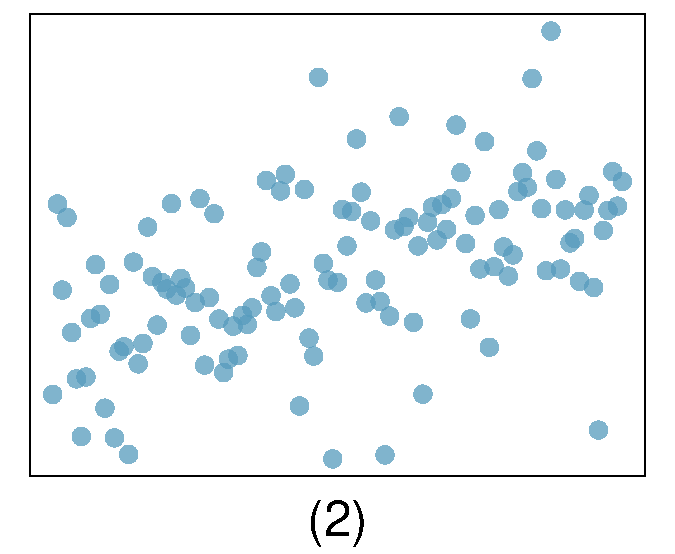
\includegraphics[width=0.245\textwidth]{ch_regr_simple_linear/figures/eoce/match_corr_2/match_corr_2_weak_pos}
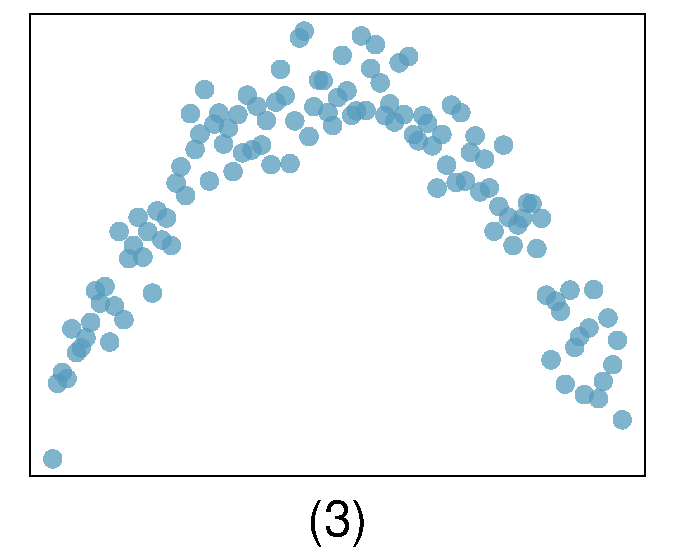
\includegraphics[width=0.245\textwidth]{ch_regr_simple_linear/figures/eoce/match_corr_2/match_corr_3_n}
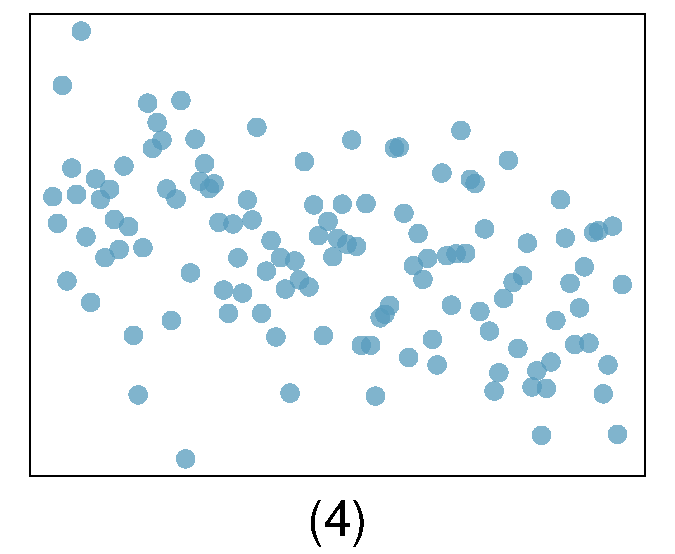
\includegraphics[width=0.245\textwidth]{ch_regr_simple_linear/figures/eoce/match_corr_2/match_corr_4_weak_neg}
\end{minipage}
}{}

% 9

\eoce{\qt{Speed and height\label{speed_height_gender}} 1,302 UCLA students 
were asked to fill out a survey where they were asked about their height, 
fastest speed they have ever driven, and gender. The scatterplot on the 
left displays the relationship between height and fastest speed, and 
the scatterplot on the right displays the breakdown by gender in 
this relationship.
\begin{center}
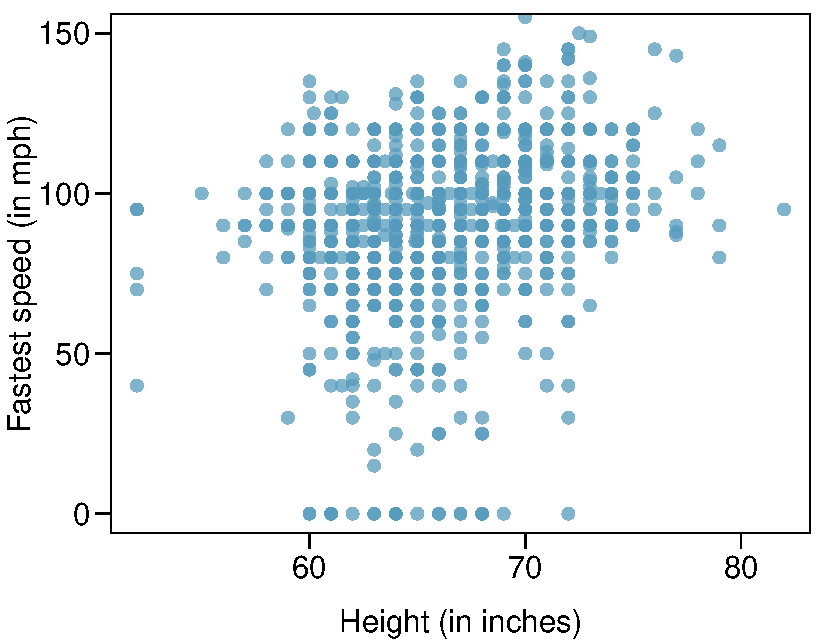
\includegraphics[width=0.43\textwidth]{ch_regr_simple_linear/figures/eoce/speed_height_gender/speed_height.pdf}
\hspace{0.02\textwidth}%
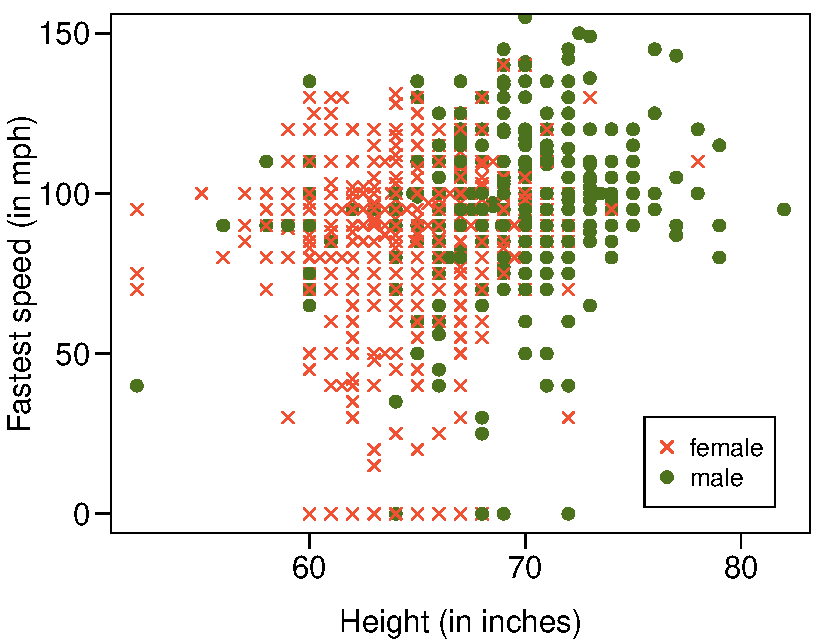
\includegraphics[width=0.43\textwidth]{ch_regr_simple_linear/figures/eoce/speed_height_gender/speed_height_gender.pdf}
\end{center}
\begin{parts}
\item Describe the relationship between height and fastest speed.
\item Why do you think these variables are positively associated?
\item What role does gender play in the relationship between height 
and fastest driving speed?
\end{parts}
}{}

\D{\newpage}
 
% 10

\eoce{\qt{Guess the correlation\label{guess_correlation}} Eduardo and Rosie 
are both collecting data on number of rainy days in a year and the total 
rainfall for the year. Eduardo records rainfall in inches and Rosie in 
centimeters. How will their correlation coefficients compare?
}{}

% 11

\eoce{\qt{The Coast Starlight, Part I\label{coast_starlight_corr_units}} 
The Coast Starlight Amtrak train runs from Seattle to Los Angeles. 
The scatterplot below displays the distance between each stop 
(in miles) and the amount of time it takes to travel from one stop 
to another (in minutes).\vspace{2mm}

\noindent\begin{minipage}[c]{0.4\textwidth}
{\raggedright\begin{parts}
\item Describe the relationship between distance and travel time.
\item How would the relationship change if travel time was instead measured 
in hours, and distance was instead measured in kilometers?
\item Correlation between travel time (in miles) and distance (in minutes) 
is $r = 0.636$. What is the correlation between travel time (in kilometers) 
and distance (in hours)?
\end{parts}\vspace{7mm}}
\end{minipage}
\begin{minipage}[c]{0.1\textwidth}
$\:$\\
\end{minipage}
\begin{minipage}[c]{0.485\textwidth}
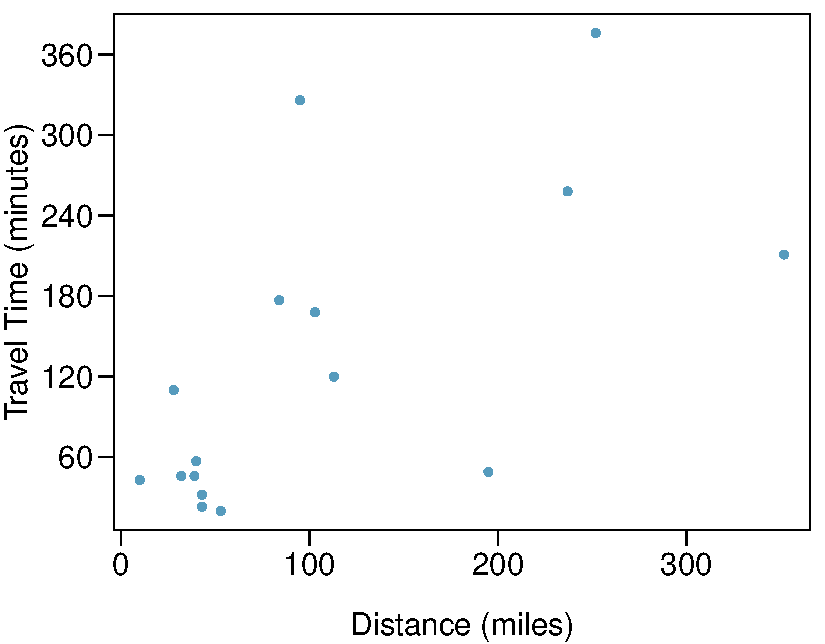
\includegraphics[width=\textwidth]{ch_regr_simple_linear/figures/eoce/coast_starlight_corr_units/coast_starlight.pdf}
\end{minipage}
}{}

% 12

\eoce{\qt{Crawling babies, Part I\label{crawling_babies_corr_units}}  
A study conducted at the University of Denver investigated whether babies 
take longer to learn to crawl in cold months, when they are often bundled 
in clothes that restrict their movement, than in warmer months.
\footfullcite{Benson:1993} Infants born during the study year were split 
into twelve groups, one for each birth month. We consider the average 
crawling age of babies in each group against the average temperature when 
the babies are six months old (that's when babies often begin trying to 
crawl). Temperature is measured in degrees Fahrenheit (\degree F) and age 
is measured in weeks.\vspace{2mm}

\noindent\begin{minipage}[c]{0.4\textwidth}
{\raggedright\begin{parts}
\item Describe the relationship between temperature and crawling age.
\item How would the relationship change if temperature was measured in 
degrees Celsius (\degree C) and age was measured in months?
\item The correlation between temperature in \degree F and age in weeks 
was $r=-0.70$. If we converted the temperature to \degree C and age to 
months, what would the correlation be?
\end{parts}\vspace{3mm}}
\end{minipage}
\begin{minipage}[c]{0.1\textwidth}
$\:$\\
\end{minipage}
\begin{minipage}[c]{0.485\textwidth}
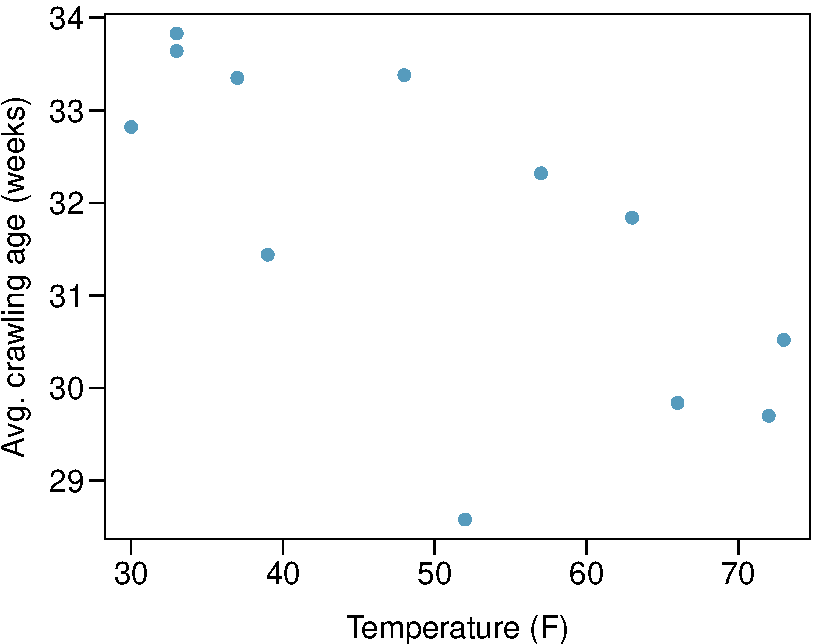
\includegraphics[width=\textwidth]{ch_regr_simple_linear/figures/eoce/crawling_babies_corr_units/crawling_babies.pdf}
\end{minipage}
}{}

\D{\newpage}
 
% 13

\eoce{\qt{Body measurements, Part I\label{body_measurements_shoulder_height_corr_units}} 
Researchers studying anthropometry collected body girth measurements and 
skeletal diameter measurements, as well as age, weight, height and gender 
for 507 physically active individuals.\footfullcite{Heinz:2003} The 
scatterplot below shows the relationship between height and shoulder 
girth (over deltoid muscles), both measured in centimeters.\vspace{3mm}

\noindent%
\begin{minipage}[c]{0.4\textwidth}
{\raggedright\begin{parts}
\item Describe the relationship between shoulder girth and height.
\item How would the relationship change if shoulder girth was measured 
in inches while the units of height remained in centimeters?
\end{parts}\vspace{20mm}}
\end{minipage}
\begin{minipage}[c]{0.1\textwidth}                  
$\:$\\
\end{minipage}
\begin{minipage}[c]{0.485\textwidth}
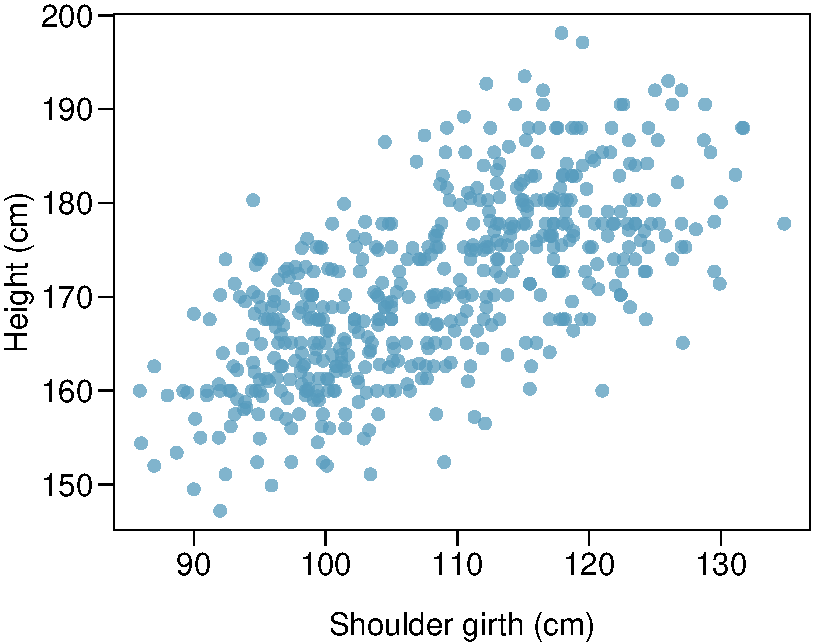
\includegraphics[width=\textwidth]{ch_regr_simple_linear/figures/eoce/body_measurements_shoulder_height_corr_units/body_measurements_height_shoulder_girth.pdf}
\end{minipage}
}{}

% 14

\eoce{\qt{Body measurements, Part II\label{body_measurements_hip_weight_corr_units}} 
The scatterplot below shows the relationship between weight 
measured in kilograms and hip girth measured in centimeters 
from the data described in 
Exercise~\ref{body_measurements_shoulder_height_corr_units}.%
\vspace{3mm}

\noindent%
\begin{minipage}[c]{0.4\textwidth}
{\raggedright\begin{parts}
\item Describe the relationship between hip girth and weight.
\item How would the relationship change if weight was measured in pounds 
while the units for hip girth remained in centimeters?
\end{parts}\vspace{20mm}}
\end{minipage}
\begin{minipage}[c]{0.1\textwidth}
$\:$\\
\end{minipage}
\begin{minipage}[c]{0.485\textwidth}
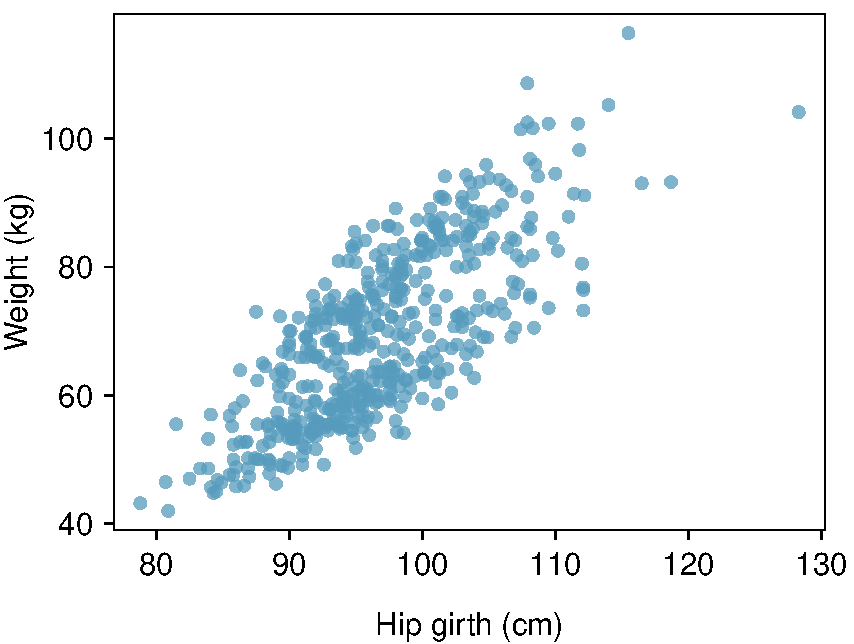
\includegraphics[width=\textwidth]{ch_regr_simple_linear/figures/eoce/body_measurements_hip_weight_corr_units/body_measurements_weight_hip_girth.pdf}
\end{minipage}
}{}

% 15

\eoce{\qt{Correlation, Part I\label{corr_husband_wife_age}} \videohref{ahss_eoce_sol-corr_husband_wife_age}\ \ What would be the 
correlation between the ages of a set of women and their spouses if the set of women always married someone who was
\begin{parts}
\item 3 years younger than themselves? 
\item 2 years older than themselves? 
\item half as old as themselves?
\end{parts}
}{}

% 16

\eoce{\qt{Correlation, Part II\label{corr_men_women_salary}} What would be the 
correlation between the annual salaries of males and females at a company 
if for a certain type of position men always made
\begin{parts}
\item \$5,000 more than women?
\item 25\% more than women?
\item 15\% less than women?
\end{parts}
}{}
}


%__________________
\section[Fitting a line by least squares regression]{Fitting a line by least squares regression }
\label{fittingALineByLSR}
\index{least squares regression|(}

\sectionintro{
\noindent%
In this section, we answer the following questions:
\begin{itemize}
\item How well can we predict financial aid based on family income for a particular college?
\item  How does one find, interpret, and apply the least squares regression line?  
\item How do we measure the fit of a model and compare different models to each other?
\item Why do models sometimes make predictions that are ridiculous or impossible?
\end{itemize}


%%
\subsection*{Learning objectives}
\begin{enumerate}
\setlength{\itemsep}{0mm}
\item Calculate the slope and y-intercept of the least squares regression line using the relevant summary statistics.  Interpret these quantities in context.

\item Understand why the least squares regression line is called the least squares regression line.

\item Interpret the explained variance $R^2$.

\item Understand the concept of extrapolation and why it is dangerous.

\item Identify outliers and influential points in a scatterplot.

\end{enumerate}
}


%%
\subsection{An objective measure for finding the best line}
Fitting linear models by eye is open to criticism since it is based on an individual preference. In this section, we use \emph{least squares regression} as a more rigorous approach.

This section considers family income and gift aid data from a random sample of fifty students in the freshman class of Elmhurst College in Illinois.\footnote{These data were sampled from a table of data for all freshmen from the 2011 class at Elmhurst College that accompanied an article titled \emph{What Students Really Pay to Go to College} published online by \emph{The~Chronicle of Higher Education}: \oiRedirect{textbook-chronicle_elmhurst_article}{chronicle.com/article/What-Students-Really-Pay-to-Go/131435}} Gift aid is financial aid that does not need to be paid back, as opposed to a loan. A scatterplot of the data is shown in Figure~\ref{elmhurstScatterW2Lines} along with two linear fits. The lines follow a negative trend in the data; students who have higher family incomes tended to have lower gift aid from the university.

\begin{figure}[h]
\centering
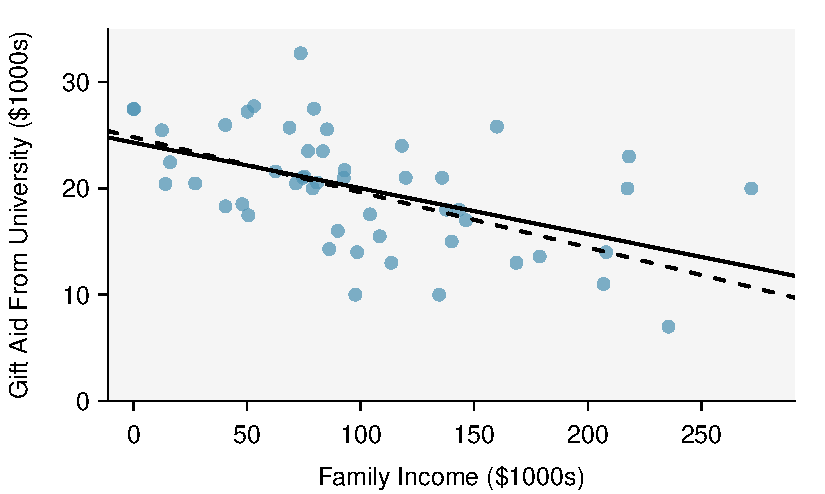
\includegraphics[width=0.7\textwidth]{ch_regr_simple_linear/figures/elmhurstPlots/elmhurstScatterW2Lines}
\caption{Gift aid and family income for a random sample of 50 freshman students from Elmhurst College. Two lines are fit to the data, the solid line being the \emph{least squares line}.}
\label{elmhurstScatterW2Lines}
\end{figure}


We begin by thinking about what we mean by ``best''. Mathematically, we want a line that has small residuals. Perhaps our criterion could minimize the sum of the residual magnitudes:
\begin{eqnarray*}
|y_1 - \hat{y}_1| + |y_2-\hat{y}_2| + \dots + |y_n-\hat{y}_n|
\label{sumOfAbsoluteValueOfResiduals}
\end{eqnarray*}
which we could accomplish with a computer program. The resulting dashed line shown in Figure~\ref{elmhurstScatterW2Lines} demonstrates this fit can be quite reasonable. However, a more common practice is to choose the line that minimizes the sum of the squared residuals:
\begin{eqnarray*}
(y_1 - \hat{y}_1)^2 + (y_2-\hat{y}_2)^2+ \dots + (y_n-\hat{y}_n)^2
\label{sumOfSquaresForResiduals}
\end{eqnarray*}
The line that minimizes the sum of the squared residuals is represented as the solid line in Figure~\ref{elmhurstScatterW2Lines}. This is commonly called the \term{least squares line}. 

Both lines seem reasonable, so why do data scientists prefer the least squares regression line?  One reason is that it is easier to compute by hand and in most statistical software.  Another, and more compelling, reason is that in many applications, a residual twice as large as another residual is more than twice as bad. For example, being off by 4 is usually more than twice as bad as being off by 2. Squaring the residuals accounts for this discrepancy.

In Figure~\ref{leastSquares}, we imagine the squared error about a line as actual squares.  The least squares regression line minimizes the sum of the \emph{areas} of these squared errors.  In the figure, the sum of the squared error is $4+1+1=6$.  There is no other line about which the sum of the squared error will be smaller.

\begin{figure}[h]
\centering
\oiRedirect{desmos-leastsquares}{
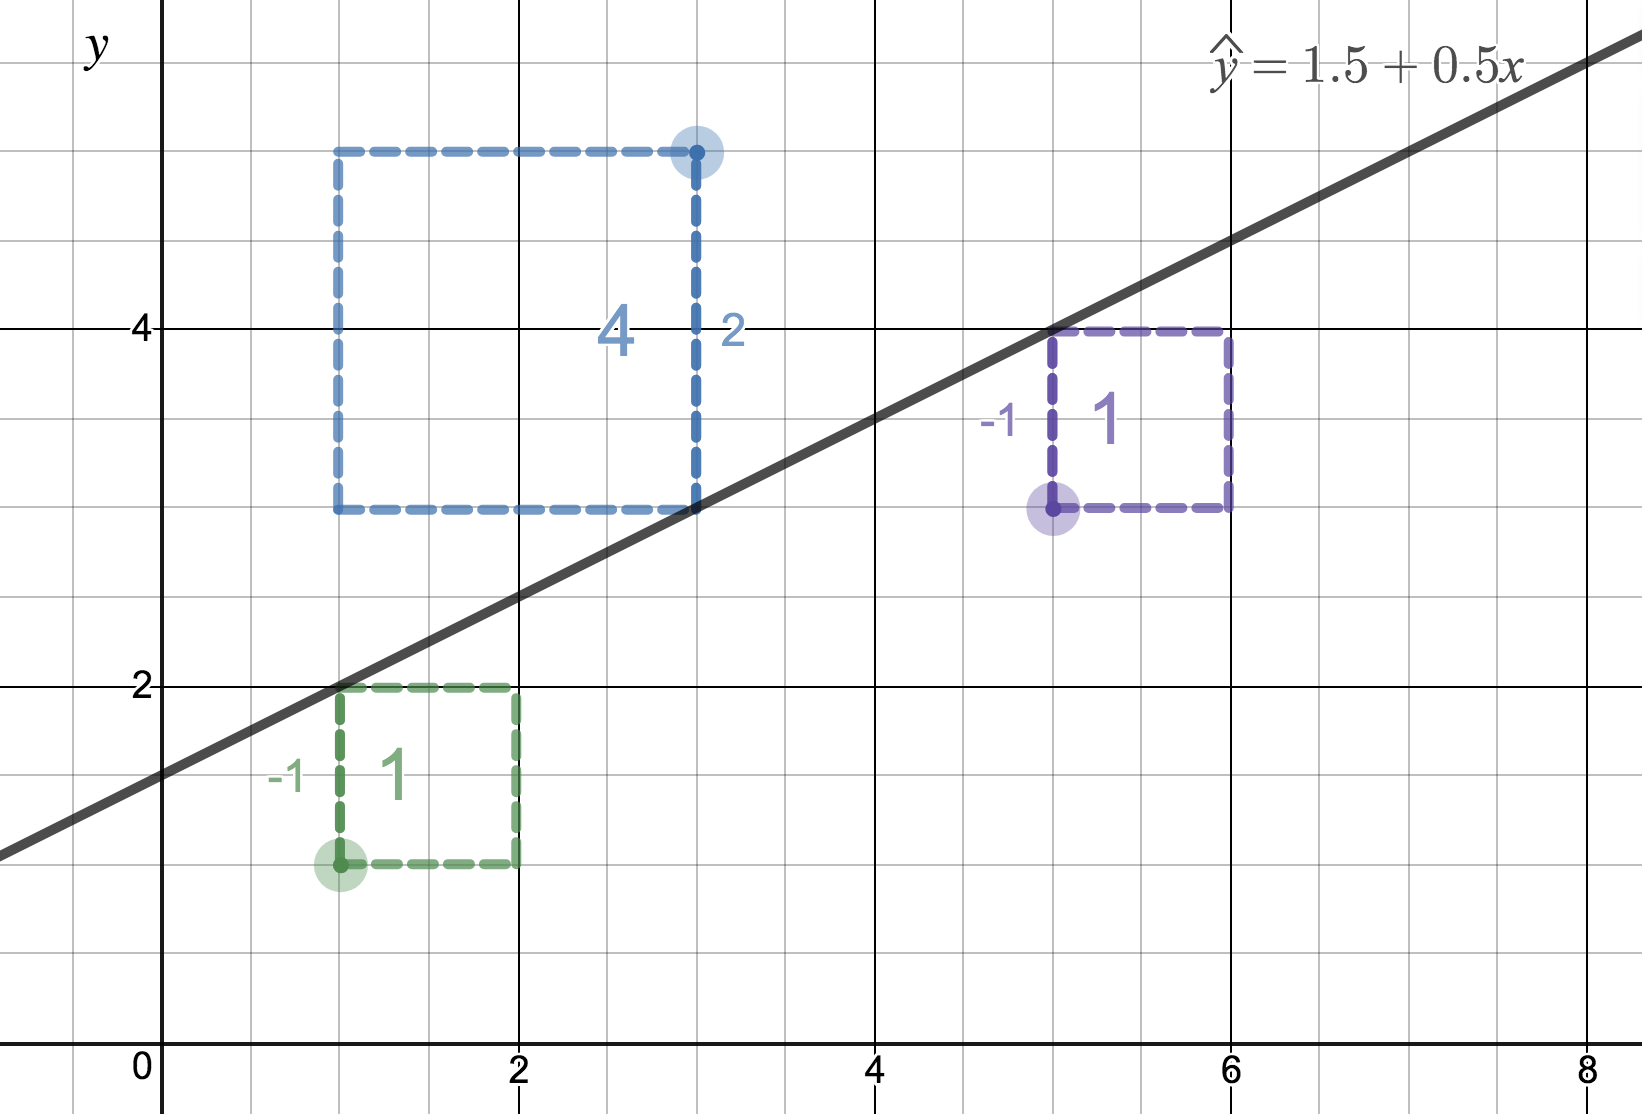
\includegraphics[width=0.75\textwidth]{ch_regr_simple_linear/figures/leastSquares/leastSquares}}
\caption{A visualization of least squares regression using Desmos.  Try out this and other interactive Desmos activities at \oiRedirect{openintro-ahss-desmos}{\small{openintro.org/ahss/desmos}}.}
\label{leastSquares}
\end{figure}


\D{\newpage}
 
%%
\subsection{Finding the least squares line}
\label{findingTheLeastSquaresLineSection}

For the Elmhurst College data, we could fit a least squares regression line for predicting gift aid based on a student's family income and write the equation as:
\begin{eqnarray*}
\widehat{\textit{aid}} = a  + b\times \textit{family\us{}income}
\end{eqnarray*}
Here $a$ is the $y$-intercept of the least squares regression line and $b$ is the slope of the least squares regression line.  $a$ and $b$ are both statistics that can be calculated from the data.  In the next section we will consider the corresponding parameters that they statistics attempt to estimate.  

We can enter all of the data into a statistical software package and easily find the values of $a$ and $b$.  However, we can also calculate these values by hand, using only the summary statistics.
\begin{itemize}
\item The slope of the least squares line is given by
\begin{eqnarray*}
b = r\frac{s_y}{s_x}
\label{slopeOfLSRLine}
\end{eqnarray*}
where $r$ is the correlation between the variables $x$ and $y$, and $s_x$ and $s_y$ are the sample standard deviations of $x$, the explanatory variable, and $y$, the response variable.
\item The point of averages $(\bar{x}, \bar{y})$ is always on the least squares line. Plugging this point in for $x$ and $y$ in the least squares equation and solving for $a$ gives
\begin{align*}
\bar{y} &= a  + b\bar{x}
&&a=\bar{y}-b\bar{x}
\label{interceptOfLSRLine}
\end{align*}
\end{itemize}


\begin{onebox}{Finding the slope and intercept of the least squares regression line}
The least squares regression line for predicting $y$ based on $x$ can be written as:  $\hat{y}=a+bx$.  
\begin{align*}
b=r\frac{s_y}{s_x} \qquad \bar{y} = a + b\bar{x}
\end{align*}
We first find $b$, the slope, and then we solve for $a$, the $y$-intercept.  
\end{onebox}

\begin{exercisewrap}
\begin{nexercise}
Figure~\ref{summaryStatsOfSATGPAData} shows the sample means for the family income and gift aid as \$101,800 and \$19,940, respectively. Plot the point $(101.8, 19.94)$ on Figure~\ref{elmhurstScatterW2Lines} to verify it falls on the least squares line (the solid line).\footnotemark 
\end{nexercise}
\end{exercisewrap}
\footnotetext{If you need help finding this location, draw a straight line up from the x-value of 100 (or thereabout). Then draw a horizontal line at 20 (or thereabout). These lines should intersect on the least squares line.}

\begin{figure}[ht]
\centering
\begin{tabular}{l rr}
\hline
\vspace{-4mm} & & \\
\vspace{0.4mm}	&	\ \ family income, in \$1000s (``$x$'')	& \ \ gift aid, in \$1000s (``$y$'') \\
\hline
  \vspace{-3.9mm} & & \\
mean	& $\bar{x} = 101.8$		& $\bar{y} = 19.94$ \\
sd		& $s_x = 63.2$		& $s_y = 5.46$\vspace{0.4mm} \\
\hline
\vspace{-4mm}\ &\\
	& \multicolumn{2}{r}{$r=-0.499$} \\
\hline
\end{tabular}
\caption{Summary statistics for family income and gift aid.}
\label{summaryStatsOfSATGPAData}
\end{figure}

\D{\newpage}
 
\begin{examplewrap}
\begin{nexample} 
{Using the summary statistics in Figure~\ref{summaryStatsOfSATGPAData}, find the equation of the least squares regression line for predicting gift aid based on family income.}
\begin{align*}
b &= r\frac{s_y}{s_x} = (-0.499)\frac{5.46}{63.2} = -0.0431 \\
a & = \bar{y} - b\bar{x} = 19.94 - (-0.0431)(101.8) = 24.3\\
\\
\hat{y}&=24.3 - 0.0431x
	\qquad\text{or}\qquad
	\widehat{\textit{aid}} = 24.3 - 0.0431\times \textit{family\us{}income}
\end{align*}
\end{nexample}
\end{examplewrap}
\label{findingTheSlopeOfTheLSRLineForIncomeAndAid}

\begin{examplewrap}
\begin{nexample}{Say we wanted to predict a student's family income based on the amount of gift aid that they received.  Would this least squares regression line be the following?
\begin{align*}
\textit{aid} = 24.3 - 0.0431\times \widehat{\textit{family\us{}income}}
\end{align*}}
No.  The equation we found was for predicting aid, not for predicting family income.  We would have to calculate a new regression line, letting $y$ be $\textit{family\us{}income}$ and $x$ be $\textit{aid}$.  This would give us:
\begin{align*}
b &= r\frac{s_y}{s_x} = (-0.499)\frac{63.2}{5.46} = -5.776 \\
a & = \bar{y} - b\bar{x} = 19.94 - (-5.776)(101.8) = 607.9\\
\\
\hat{y}&=607.3 - 5.776x
	\qquad\text{or}\qquad
	\widehat{\textit{family\us{}income}} = 607.3 - 5.776\times \textit{aid}
\end{align*}

\end{nexample}
\end{examplewrap} 


We mentioned earlier that a computer is usually used to compute the least squares line. A summary table based on computer output is shown in Figure~\ref{rOutputForIncomeAidLSRLine} for the Elmhurst College data. The first column of numbers provides estimates for ${b}_0$ and ${b}_1$, respectively. Compare these to the result from Example~\ref{findingTheSlopeOfTheLSRLineForIncomeAndAid}.

\begin{figure}[ht]
\centering
\begin{tabular}{l rrrr}
  \hline
  \vspace{-3.7mm} & & & & \\
 & Estimate & Std. Error & t value & Pr($>$$|$t$|$) \\ 
  \hline
  \vspace{-3.6mm} & & & & \\
(Intercept) & 24.3193 & 1.2915 & 18.83 & 0.0000 \\ 
family\us{}income & -0.0431 & 0.0108 & -3.98 & 0.0002 \\ 
  \hline
\end{tabular}
\caption{Summary of least squares fit for the Elmhurst College data. Compare the parameter estimates in the first column to the results of Guided Practice~\ref{findingTheSlopeOfTheLSRLineForIncomeAndAid}.}
\label{rOutputForIncomeAidLSRLine}
\end{figure}

\begin{examplewrap}
\begin{nexample}{Examine the second, third, and fourth columns in Figure~\ref{rOutputForIncomeAidLSRLine}. Can you guess what they represent?}
We'll look at the second row, which corresponds to the slope.  The first column, Estimate = -0.0431, tells us our best estimate for the slope of the population regression line.  We call this point estimate $b$.  The second column, Std. Error = 0.0108, is the standard error of this point estimate. The third column, t value = -3.98, is the $T$ test statistic for the null hypothesis that the slope of the population regression line = 0. The last column, Pr($>$$|$t$|$) = 0.0002, is the p-value for this two-sided $T$-test. We will get into more of these details in Section~\ref{inferenceForLinearRegression}.
\end{nexample}
\end{examplewrap}

\begin{examplewrap}
\begin{nexample}{Suppose a high school senior is considering Elmhurst College. Can she simply use the linear equation that we have found to calculate her financial aid from the university?}
No.  Using the equation will provide a prediction or estimate.  However, as we see in the scatterplot, there is a lot of variability around the line.  While the linear equation is good at capturing the trend in the data, there will be significant error in predicting an individual student's aid.  Additionally, the data all come from one freshman class, and the way aid is determined by the university may change from year to year.
\end{nexample}
\end{examplewrap} 


%%
\subsection{Interpreting the coefficients of a regression line}

\index{least squares regression!interpreting parameters|(}

Interpreting the coefficients in a regression model is often one of the most important steps in the analysis.

\begin{examplewrap}
\begin{nexample}{The slope for the Elmhurst College data for predicting gift aid based on family income was calculated as -0.0431.  Intepret this quantity in the context of the problem. }
You might recall from an algebra course that slope is change in $y$ over change in $x$.  Here, both $x$ and $y$ are in thousands of dollars.  So if $x$ is one unit or one thousand dollars higher, the line will predict that $y$ will change by 0.0431 thousand dollars.  In other words, for each additional thousand dollars of family income, \emph{on average}, students receive 0.0431 thousand, or \$43.10 \emph{less} in gift aid. Note that a higher family income corresponds to less aid because the slope is negative.   
\end{nexample}
\end{examplewrap}

\begin{examplewrap}
\begin{nexample}{The $y$-intercept for the Elmhurst College data for predicting gift aid based on family income was calculated as 24.3.  Intepret this quantity in the context of the problem. }
The intercept $a$ describes the predicted value of $y$ when $x=0$.  The \emph{predicted} gift aid is 24.3 thousand dollars if a student's family has no income.  The meaning of the intercept is relevant to this application since the family income for some students at Elmhurst is \$0. In other applications, the intercept may have little or no practical value if there are no observations where $x$ is near zero.  Here, it would be acceptable to say that the \emph{average} gift aid is 24.3 thousand dollars among students whose family have 0 dollars in income.
\end{nexample}
\end{examplewrap}

\begin{onebox}{Interpreting coefficients in a linear model}
\vspace{-4mm}
\begin{itemize}
\setlength{\itemsep}{0mm}
\item The slope, $b$, describes the \emph{average} increase or decrease in the $y$ variable if the explanatory variable $x$ is one unit larger. 
\item The y-intercept, $a$, describes the predicted outcome of $y$ if $x=0$.  The linear model must be valid all the way to $x=0$ for this to make sense, which in many applications is not the case.
\end{itemize}
\end{onebox}

\index{least squares regression!interpreting parameters|)}

\begin{exercisewrap}
\begin{nexercise}
In the previous chapter, we encountered a data set that compared the price of new textbooks for UCLA courses at the UCLA Bookstore and on Amazon.  We fit a linear model for predicting price at UCLA Bookstore from price on Amazon and we get:  
\begin{align*}
\hat{y} = 1.86 + 1.03x
\end{align*}
where $x$ is the price on Amazon and $y$ is the price at the UCLA bookstore.  Interpret the coefficients in this model and discuss whether the interpretations make sense in this context.\footnotemark
\end{nexercise}
\end{exercisewrap}
\footnotetext{The $y$-intercept is 1.86 and the units of $y$ are in dollars.  This tells us that when a textbook costs 0 dollars on Amazon, the predicted price of the textbook at the UCLA Bookstore is 1.86 dollars.  This does not make sense as Amazon does not sell any \$0 textbooks.  The slope is 1.03, with units (dollars)/(dollars).  On average, for every extra dollar that a book costs on Amazon, it costs an extra 1.03 dollars at the UCLA Bookstore.  This interpretation does make sense in this context.
}


\begin{exercisewrap}
\begin{nexercise}
Can we conclude that if Amazon raises the price of a textbook by 1 dollar, the UCLA Bookstore will raise the price of the textbook by \$1.03?\footnotemark
\end{nexercise}
\end{exercisewrap}
\footnotetext{No.  The slope describes the overall trend.  This is observational data; a causal conclusion cannot be drawn.  Remember, a causal relationship can only be concluded by a well-designed randomized, controlled experiment.  Additionally, there may be large variation in the points about the line.  The slope does not tell us how much $y$ might change based on a change in $x$ for a particular textbook.
}

\begin{onebox}{Exercise caution when interpreting coefficients of a linear model}
\vspace{-4mm}
\begin{itemize}
\setlength{\itemsep}{0mm}
\item The slope tells us only the \emph{average} change in $y$ for each unit change in $x$; it does not tell us how much $y$ might change based on a change in $x$ for any particular \emph{individual}.  Moreover, in most cases, the slope cannot be interpreted in a causal way.
\item When a value of $x=0$ doesn't make sense in an application, then the interpretation of the $y$-intercept won't have any practical meaning.  
\end{itemize}
\end{onebox}


%%
\subsection{Extrapolation is treacherous}
\index{least squares regression!extrapolation|(}

{\em\small When those blizzards hit the East Coast this winter, it proved to my satisfaction that global warming was a fraud. That snow was freezing cold. But in an alarming trend, temperatures this spring have risen. Consider this: On February $6^{th}$ it was 10 degrees. Today it hit almost 80. At this rate, by August it will be 220 degrees. So clearly folks the climate debate rages on.\vspace{0.5mm}}

\noindent\hspace{\textwidth}\hspace{-40mm}Stephen Colbert

\noindent\hspace{\textwidth}\hspace{-40mm}April 6th, 2010 \footnote{\oiRedirect{textbook-colbert_extrapolation}{www.cc.com/video-clips/l4nkoq/}} \\

Linear models can be used to approximate the relationship between two variables. However, these models have real limitations. Linear regression is simply a modeling framework. The truth is almost always much more complex than our simple line. For example, we do not know how the data outside of our limited window will behave.

\D{\newpage}

\begin{examplewrap}
\begin{nexample}{Use the model $\widehat{\textit{aid}} = 24.3 - 0.0431\times \textit{family\us{}income}$ to estimate the aid of another freshman student whose family had income of \$1 million.}
Recall that the units of family income are in \$1000s, so we want to calculate the aid for $\textit{family\us{}income}= 1000$:
\begin{align*}
\widehat{\textit{aid}} &= 24.3 - 0.0431 \times \textit{family\us{}income} \\
\widehat{\textit{aid}}&=24.3 - 0.431(1000) = -18.8
\end{align*}
The model predicts this student will have -\$18,800 in aid (!). Elmhurst College cannot (or at least does not) require any students to pay extra on top of tuition to attend.
\end{nexample}
\end{examplewrap}

Using a model to predict $y$-values for $x$-values outside the domain of the original data is called \term{extrapolation}. Generally, a linear model is only an approximation of the real relationship between two variables. If we extrapolate, we are making an unreliable bet that the approximate linear relationship will be valid in places where it has not been analyzed.

\index{least squares regression!extrapolation|)}



%%
\subsection[Using $R^2$ to describe the strength of a fit]{Using \pmb{$R^2$} to describe the strength of a fit}

\index{least squares regression!R-squared ($R^2$)|(}

We evaluated the strength of the linear relationship between two variables earlier using the correlation, $r$. However, it is more common to explain the fit of a model using $R^2$, called \termsub{R-squared}{least squares regression!R-squared ($R^2$)} or the \term{explained variance}. If provided with a linear model, we might like to describe how closely the data cluster around the linear fit.


\begin{figure}[h]
\centering
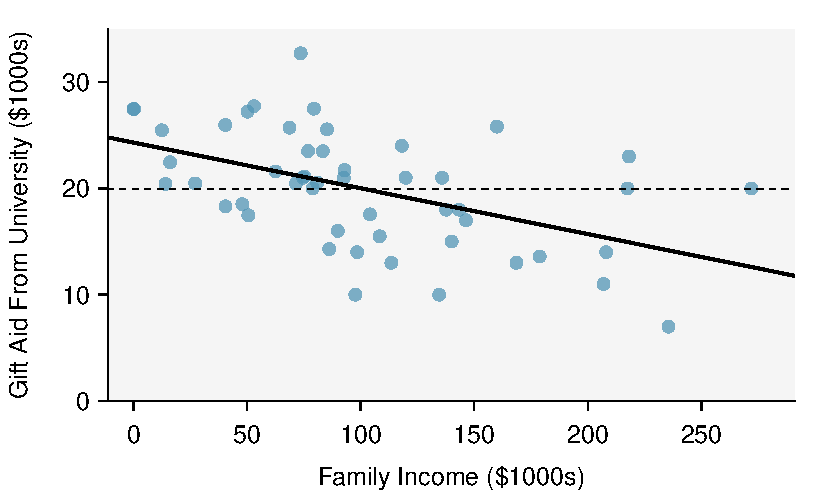
\includegraphics[width=0.7\textwidth]{ch_regr_simple_linear/figures/elmhurstPlots/elmhurstScatterWAveLine}
\caption{Gift aid and family income for a random sample of 50 freshman students from Elmhurst College, shown with the least squares regression line ($\hat{y}$) and the average line ($\bar{y}$).}
\label{elmhurstScatterWLSROnly}
\end{figure}

We are interested in how well a model accounts for or explains the location of the $y$ values.
The $R^2$ of a linear model describes how much smaller the variance (in the $y$ direction) about the regression line is than the variance about the horizontal line $\bar{y}$.
For example, consider the Elmhurst College data, shown in Figure~\ref{elmhurstScatterWLSROnly}. The variance of the response variable, aid received, is $s_{aid}^2=29.8$. However, if we apply our least squares line, then this model reduces our uncertainty in predicting aid using a student's family income. The variability in the residuals describes how much variation remains after using the model: $s_{_{RES}}^2 = 22.4$.
We could say that the reduction in the variance was:
$$\frac{s_{aid}^2 - s_{_{RES}}^2}{s_{aid}^2}
	= \frac{29.8 - 22.4}{29.8} = \frac{7.5}{29.8}
	= 0.25$$
If we used the simple standard deviation of the
residuals, this would be exactly $R^2$.
However, the standard way of computing the standard deviation of the residuals is slightly more sophisticated.\footnote{In computing the standard deviation of the residuals, we divide by $n-2$ rather than by $n-1$ to account for the $n-2$ degrees of freedom.}
To avoid any trouble, we can instead use a sum of squares method.
If we call the sum of the squared errors about the regression line $SSRes$ and the sum of the squared errors about the mean $SSM$, we can define $R^2$ as follows:
\begin{align*}
R^2=\frac{SSM - SSRes}{SSM} = 1-\frac{SSRes}{SSM}
\end{align*}


\begin{figure}[ht]
  \centering
\oiRedirect{desmos-rsquared}{
  \subfigure[]{
    \Figures{0.4}
        {rSquared}
        {rsq1}
    \label{rsq1}
  }\hspace{5mm}
  \subfigure[]{
    \Figures{0.4}
        {rSquared}
        {rsq2}
  \label{rsq2}
  }}
  \caption{\subref{rsq1} The regression line is equivalent to $\bar{y}$; $R^2 = 0$.
      \subref{rsq2} The regression line passes through all of the points; $R^2=1$.  Try out this and other interactive Desmos activities at \oiRedirect{openintro-ahss-desmos}{\small{openintro.org/ahss/desmos}}.}
    \label{rSquared}
\end{figure}

\begin{exercisewrap}
\begin{nexercise}
Using the formula for $R^2$, confirm that in Figure~\ref{rSquared} (a), $R^2 = 0$ and that in Figure~\ref{rSquared} (b), $R^2 = 1$.\footnotemark
\end{nexercise}
\end{exercisewrap}
\footnotetext{(a) $SSRes = SSM = (-1)^2 +(2)^2+(-1)^2=6$, so $R^2 = 1 - \frac{6}{6}=0$.  (b) $R^2 = 1- \frac{0}{8}$.}

\begin{onebox}{\pmb{$R^2$} is the explained variance}
$R^2$ is always between 0 and 1, inclusive.  It tells us the proportion of variation in the $y$ values that is explained by a regression model.  The higher the value of $R^2$, the better the model ``explains" the response variable.
\end{onebox}

The value of $R^2$ is, in fact, equal to $r^2$, where $r$ is the correlation.  This means that  $r = \pm \sqrt{R^2}$.  Use this fact to answer the next two practice problems.

\begin{exercisewrap}
\begin{nexercise}
If a linear model has a very strong negative relationship with a correlation of -0.97, how much of the variation in the response variable is explained by the linear model?\footnotemark 
\end{nexercise}
\end{exercisewrap}
\footnotetext{$R^2 = (-0.97)^2 = 0.94$ or 94\%.  94\% of the variation in $y$ is explained by the linear model.}
\index{least squares regression!R-squared ($R^2$)|)}

\begin{exercisewrap}
\begin{nexercise}
If a linear model has an $R^2$ or explained variance of 0.94, what is the correlation?\footnotemark 
\end{nexercise}
\end{exercisewrap}
\footnotetext{We take the square root of $R^2$ and get 0.97, but we must be careful, because $r$ could be 0.97 \emph{or} -0.97.  Without knowing the slope or seeing the scatterplot, we have no way of knowing if $r$ is positive or negative.}

%%
\subsection{Calculator/Desmos: linear correlation and regression}
\label{calclinreg}

\begin{onebox}{\videohref{ti84_calculating_regression_summary_statistics} TI-84: finding $\MakeLowercase{\pmb{a}}$, \MakeLowercase{\pmb{$b$}}, $\pmb{R^2}$, and \MakeLowercase{\pmb{$r$}} for a linear model}
Use \calctext{STAT}, \calctext{CALC}, \calctext{LinReg(a + bx)}.
\begin{enumerate}
\setlength{\itemsep}{0mm}
\item Choose \calctext{STAT}.
\item Right arrow to \calctext{CALC}.
\item Down arrow and choose \calctext{8:LinReg(a+bx)}.\vspace{-1.5mm}
  \begin{itemize}
  \item Caution: choosing \calctext{4:LinReg(ax+b)} will reverse $a$ and $b$.
  \end{itemize}
\item Let \calctext{Xlist} be \calctext{L1} and \calctext{Ylist} be \calctext{L2} (don't forget to enter the $x$ and $y$ values in L1 and \calctext{L2} before doing this calculation).  
\item Leave \calctext{FreqList} blank.
\item Leave \calctext{Store RegEQ} blank.
\item Choose Calculate and hit \calctext{ENTER}, which returns: \\[1mm]
\begin{tabular}{l l}
\calctext{a} & $a$, the y-intercept of the best fit line \\
\calctext{b} & $b$, the slope of the best fit line \\
$\calctextmath{r^2}$ & $R^2$, the explained variance \\
\calctext{r} & $r$, the correlation coefficient
\end{tabular}
\end{enumerate}
TI-83: Do steps 1-3, then enter the $x$ list and $y$ list separated by a comma, e.g. \calctext{LinReg(a+bx) L1, L2}, then hit \calctext{ENTER}.\end{onebox} 

\begin{onebox}{What to do if \pmb{$r^2$} and \MakeLowercase{\pmb{$r$}} do not show up on a TI-83/84}
If $r^2$ and $r$ do now show up when doing \calctext{STAT}, \calctext{CALC}, \calctext{LinReg}, the \emph{diagnostics} must be turned on.  This only needs to be once and the diagnostics will remain on.
\begin{enumerate}
\setlength{\itemsep}{0mm}
\item Hit \calctext{2ND} \calctext{0} (i.e. \calctext{CATALOG}).
\item Scroll down until the arrow points at \calctext{DiagnosticOn}.
\item Hit \calctext{ENTER} and \calctext{ENTER} again. The screen should now say: \\[1mm]
\begin{tabular}{l l}
\calctext{DiagnosticOn}& \\
&\calctext{Done} \\
\end{tabular}
\end{enumerate}
\end{onebox} 

\begin{onebox}{What to do if a TI-83/84 returns: {ERR:}~{DIM MISMATCH}}
\label{dimmismatch}
This error means that the lists, generally L1 and L2, do not have the same length.
\begin{enumerate}
\setlength{\itemsep}{0mm}
\item Choose \calctext{1:Quit}.
\item Choose \calctext{STAT},~\calctext{Edit} and make sure that the lists have the same number of entries.
\end{enumerate}
\end{onebox} 

\begin{onebox}{\videohref{casio_calculating_regression_summary_statistics} Casio fx-9750GII: finding $\MakeLowercase{\pmb{a}}$, \MakeLowercase{\pmb{$b$}}, $\pmb{R^2}$, and \MakeLowercase{\pmb{$r$}} for a linear model}
\begin{enumerate}
\setlength{\itemsep}{0mm}
\item Navigate to \calctext{STAT} (\calcbutton{MENU} button, then hit the \calcbutton{2} button or select \calctext{STAT}).
\item Enter the $x$ and $y$ data into 2 separate lists, e.g. $x$ values in \calctext{List 1} and $y$ values in \calctext{List 2}. Observation ordering should be the same in the two lists. For example, if $(5, 4)$ is the second observation, then the second value in the $x$ list should be 5 and the second value in the $y$ list should be 4.
\item Navigate to \calctext{CALC} (\calcbutton{F2}) and then \calctext{SET} (\calcbutton{F6}) to set the regression context.\vspace{-1.5mm}
  \begin{itemize}
  \item To change the \calctext{2Var XList}, navigate to it, select \calctext{List} (\calcbutton{F1}), and enter the proper list number. Similarly, set \calctext{2Var YList} to the proper list.
  \end{itemize}
\item Hit \calcbutton{EXIT}.
\item Select \calctext{REG} (\calcbutton{F3}), \calctext{X} (\calcbutton{F1}), and \calctext{a+bx} (\calcbutton{F2}), which returns: \\[1mm]
\begin{tabular}{l l}
\calctext{a} & $a$, the y-intercept of the best fit line \\
\calctext{b} & $b$, the slope of the best fit line \\
\calctext{r} & $r$, the correlation coefficient \\
$\calctextmath{r^2}$ & $R^2$, the explained variance \\
\calctext{MSe} & Mean squared error, which you can ignore
\end{tabular} \\[1mm]
If you select \calctext{ax+b} (\calcbutton{F1}), the \calctext{a} and \calctext{b} meanings will be reversed.
\end{enumerate}\end{onebox} 




\begin{exercisewrap}
\begin{nexercise}\label{subsetOfLoan50}%
The data set \data{loan50}, introduced in Chapter 1, contains information on randomly sampled loans offered through Lending Club.  A subset of the data matrix is shown in
Figure~\ref{data_for_regr_calc_exercise_loan50}.  Use a calculator to find the equation of the least squares regression line for predicting loan amount from total income.\footnotemark 
\end{nexercise}
\end{exercisewrap}
\footnotetext{$\calctext{a}=11121$ and $\calctext{b}=0.0043$, therefore $\hat{y}=11121 + 0.0043x$.}

\begin{figure}[ht]
\centering
\begin{tabular}{rrr}
  \hline
 & total\_income & loan\_amount \\ 
  \hline
1 & 59000 & 22000 \\ 
  2 & 60000 & 6000 \\ 
  3 & 75000 & 25000 \\ 
  4 & 75000 & 6000 \\ 
  5 & 254000 & 25000 \\ 
  6 & 67000 & 6400 \\ 
  7 & 28800 & 3000 \\ 
   \hline
\end{tabular}
\caption{Sample of data from \data{loan50}.}
\label{data_for_regr_calc_exercise_loan50}
\end{figure}


\D{\newpage}

\begin{examplewrap}
\begin{nexample}
{Use the full \data{loan50} data set (\oiRedirect{data}{\small{openintro.org/ahss/data}}) and this \oiRedirect{desmos-linregcalculator}{Desmos Calculator} \mbox{(\small{openintro.org/ahss/desmos})} to draw the scatterplot and find the equation of the least squares regression line for prediction loan amount ($y$) from total income ($x$).}
\begin{center}
\oiRedirect{desmos-loan50scatter}{
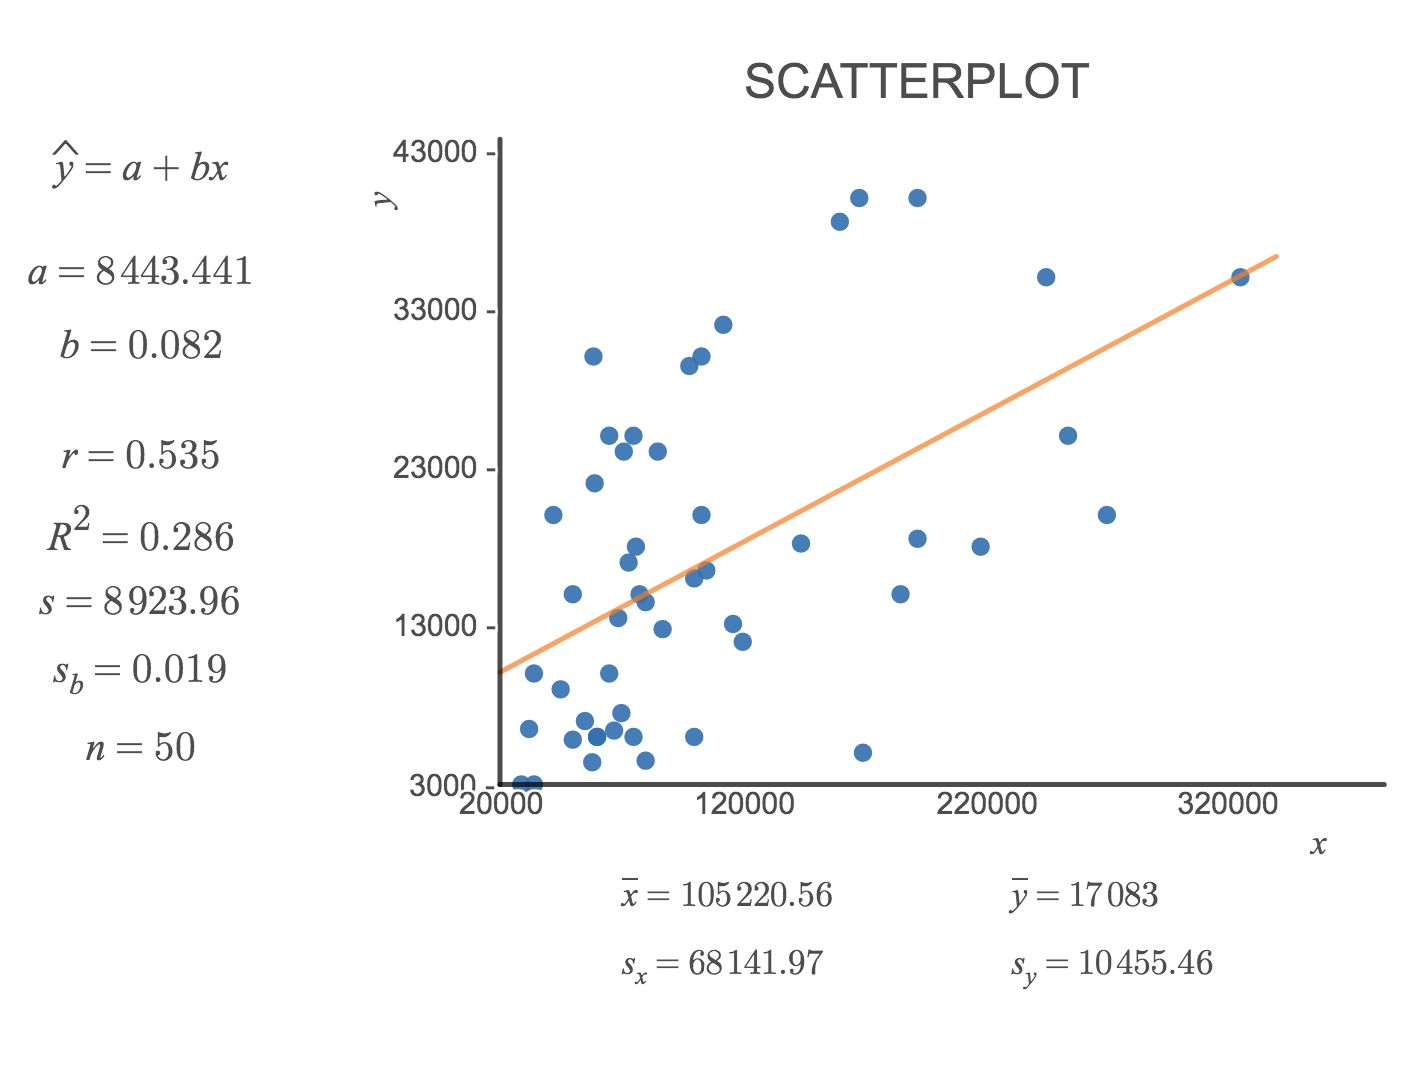
\includegraphics[width=0.75\textwidth]{ch_regr_simple_linear/figures/loan50Desmos/loan50Desmos}}
\end{center}
\end{nexample}
\end{examplewrap}
\label{loan50Desmos}
\D{\newpage}

%%%%
\subsection{Types of outliers in linear regression }
\label{typesOfOutliersInLinearRegression}

Outliers in regression are observations that fall far from the ``cloud'' of points. These points are especially important because they can have a strong influence on the least squares line. 

\begin{examplewrap}
\begin{nexample}{There are six plots shown in Figure~\ref{outlierPlots} along with the least squares line and residual plots. For each scatterplot and residual plot pair, identify any obvious outliers and note how they influence the least squares line. Recall that an outlier is any point that doesn't appear to belong with the vast majority of the other points.}\label{outlierPlotsExample}
\begin{itemize}
\setlength{\itemsep}{0mm}
\item[(1)] There is one outlier far from the other points, though it only appears to slightly influence the line.
\item[(2)] There is one outlier on the right, though it is quite close to the least squares line, which suggests it wasn't very influential.
\item[(3)] There is one point far away from the cloud, and this outlier appears to pull the least squares line up on the right; examine how the line around the primary cloud doesn't appear to fit very well.
\item[(4)] There is a primary cloud and then a small secondary cloud of four outliers. The secondary cloud appears to be influencing the line somewhat strongly, making the least squares line fit poorly almost everywhere. There might be an interesting explanation for the dual clouds, which is something that could be investigated.
\item[(5)] There is no obvious trend in the main cloud of points and the outlier on the right appears to largely control the slope of the least squares line.
\item[(6)] There is one outlier far from the cloud, however, it falls quite close to the least squares line and does not appear to be very influential.
\end{itemize}
\end{nexample}
\end{examplewrap}

\begin{figure}
\centering
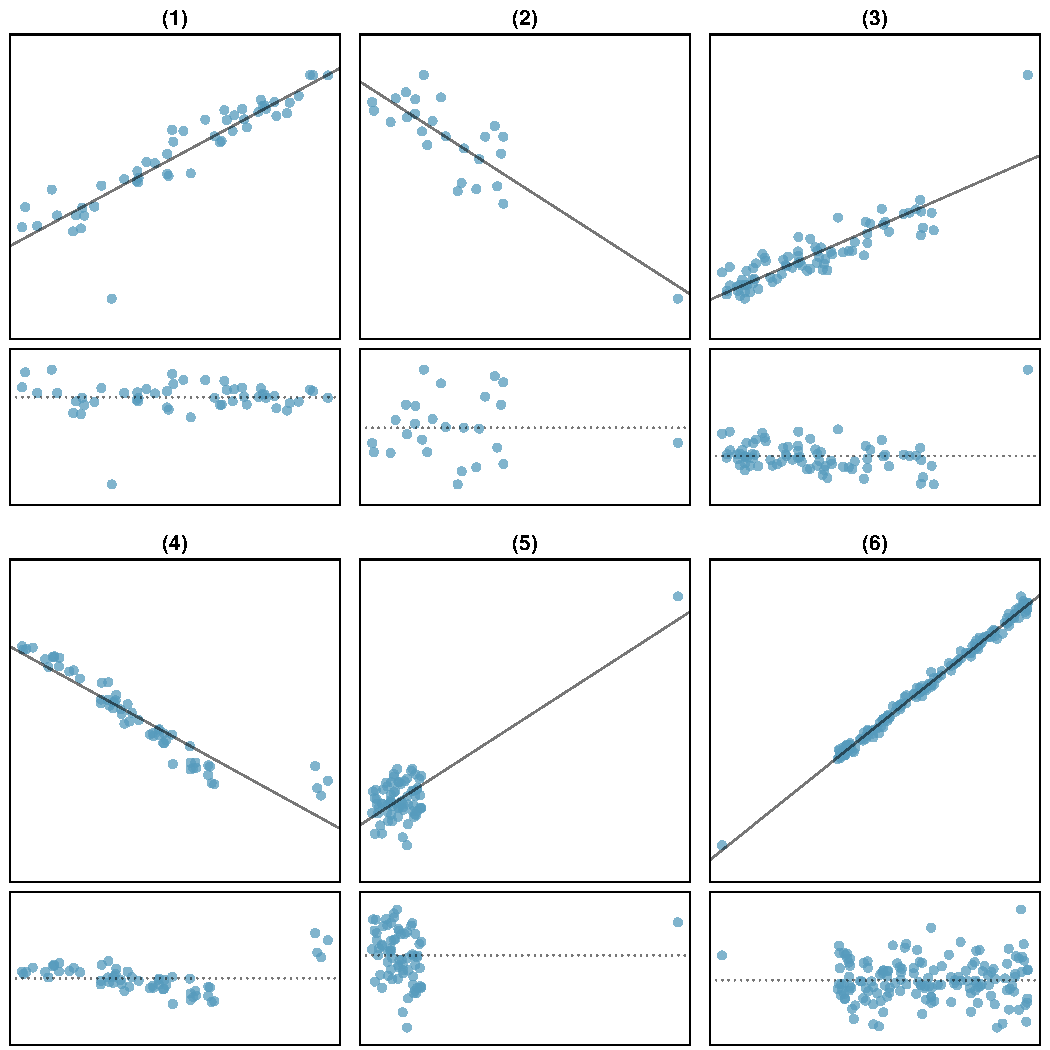
\includegraphics[width=\textwidth]{ch_regr_simple_linear/figures/outlierPlots/outlierPlots}
\caption{Six plots, each with a least squares line and residual plot. All data sets have at least one outlier.}
\label{outlierPlots}
\end{figure}


Examine the residual plots in Figure~\ref{outlierPlots}. You will probably find that there is some trend in the main clouds of (3) and (4). In these cases, the outliers influenced the slope of the least squares lines. In (5), data with no clear trend were assigned a line with a large trend simply due to one outlier (!).
 
 \begin{onebox}{Leverage}
Points that fall horizontally away from the center of the cloud tend to pull harder on the line, so we call them points with \term{high leverage}.\end{onebox}

Points that fall horizontally far from the line are points of high leverage; these points can strongly influence the slope of the least squares line. If one of these high leverage points does appear to actually invoke its influence on the slope of the line -- as in cases (3), (4), and (5) of Example~\ref{outlierPlotsExample} -- then we call it an \term{influential point}. Usually we can say a point is influential if, had we fitted the line without it, the influential point would have been unusually far from the least squares line.

It is tempting to remove outliers. Don't do this without a very good reason. Models that ignore exceptional (and interesting) cases often perform poorly. For instance, if a financial firm ignored the largest market swings -- the ``outliers'' --  they would soon go bankrupt by making poorly thought-out investments.

\begin{onebox}{Don't ignore outliers when fitting a final model}
{If there are outliers in the data, they should not be removed or ignored without a~good reason. Whatever final model is fit to the data would not be very helpful if it ignores the most exceptional cases.}
\end{onebox}


\D{\newpage}

%%
\subsection{Categorical predictors with two levels (special topic)}
\label{categoricalPredictorsWithTwoLevels}
Categorical variables are also useful in predicting outcomes. Here we consider a categorical predictor with two levels (recall that a \emph{level} is the same as a \emph{category}). We'll consider eBay auctions for a video game, \emph{Mario Kart} for the Nintendo Wii, where both the total price of the auction and the condition of the game were recorded.\footnote{These data were collected in Fall 2009 and may be found at \oiRedirect{textbook-openintro_org_stat}{openintro.org/stat}.} Here we want to predict total price based on game condition, which takes values \resp{used} and \resp{new}. A plot of the auction data is shown in Figure~\ref{marioKartNewUsed}.

\begin{figure}[h]
\centering
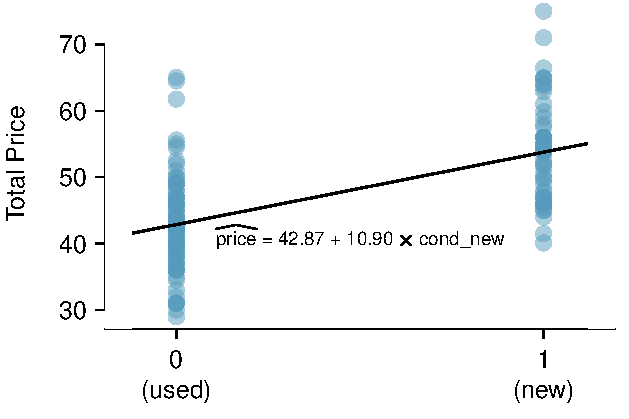
\includegraphics[width=0.49\textwidth]{ch_regr_simple_linear/figures/marioKartNewUsed/marioKartNewUsed}
\caption{Total auction prices for the game \emph{Mario Kart}, divided into used ($x=0$) and new ($x=1$) condition games with the least squares regression line~shown.}
\label{marioKartNewUsed}
\end{figure}

To incorporate the game condition variable into a regression equation, we must convert the categories into a numerical form. We will do so using an \term{indicator variable} called \var{cond\us{}new}, which takes value 1 when the game is new and 0 when the game is used. Using this indicator variable, the linear model may be written as
\begin{align*}
\widehat{price} = \alpha + \beta \times \text{\var{cond\us{}new}}
\end{align*}
The fitted model is summarized in Figure~\ref{marioKartNewUsedRegrSummary}, and the model with its parameter estimates is given~as
\begin{align*}
\widehat{price} = 42.87 + 10.90 \times \text{\var{cond\us{}new}}
\end{align*}
For categorical predictors with two levels, the linearity assumption will always be satisfied.
However, we must evaluate whether the residuals in each group are approximately normal with equal variance.
Based on Figure~\ref{marioKartNewUsed}, both of these conditions are reasonably satisfied.

\begin{figure}[h]
\centering
\begin{tabular}{rrrrr}
  \hline
  \vspace{-3.7mm} & & & & \\
 & Estimate & Std. Error & t value & Pr($>$$|$t$|$) \\ 
  \hline
  \vspace{-3.6mm} & & & & \\
(Intercept) & 42.87 & 0.81 & 52.67 & 0.0000 \\ 
  cond\us{}new & 10.90 & 1.26 & 8.66 & 0.0000 \\ 
   \hline
\end{tabular}
\caption{Least squares regression summary for the Mario Kart data.}
\label{marioKartNewUsedRegrSummary}
\end{figure}

\begin{examplewrap}
\begin{nexample}{Interpret the two parameters estimated in the model for the price of \emph{Mario Kart} in eBay auctions.}
The intercept is the estimated price when \var{cond\us{}new} takes value 0, i.e. when the game is in used condition. That~is, the average selling price of a used version of the game is \$42.87.

The slope indicates that, on average, new games sell for about \$10.90 more than used games.
\end{nexample}
\end{examplewrap}

\begin{onebox}{Interpreting model estimates for categorical predictors.}
The estimated intercept is the value of the response variable for the first category (i.e. the category corresponding to an indicator value of 0). The estimated slope is the average change in the response variable between the two categories.\end{onebox}


\D{\newpage}
 
%%
\subsection*{Section summary}

\begin{itemize}
\item We define the \emph{best fit line} as the line that minimizes the sum of the squared residuals (errors) about the line.  That~is, we find the line that minimizes $(y_1 - \hat{y}_1)^2 + (y_2-\hat{y}_2)^2+ \dots + (y_n-\hat{y}_n)^2=\sum{(y_i - \hat{y}_i)^2}$. We call this line the \term{least squares regression line}.

\item We write the least squares regression line in the form: $\hat{y} = a  + bx$,  and we can calculate $a$ and $b$ based on the summary statistics as follows:
\begin{eqnarray*}
b=r\frac{s_y}{s_x} \qquad \text{and} \qquad a=\bar{y} - b\bar{x}.
\end{eqnarray*}

\item \emph{Interpreting} the \term{slope} and \term{y-intercept} of a linear model
\begin{itemize}
\item The slope, $b$, describes the \emph{average} increase or decrease in the $y$ variable if the explanatory variable $x$ is one unit larger. 
\item The y-intercept, $a$, describes the average or predicted outcome of $y$ if $x=0$.  The linear model must be valid all the way to $x=0$ for this to make sense, which in many applications is not the case.
\end{itemize}

\item Two important considerations about the regression line
\begin{itemize}
\item  The regression line provides \textit{estimates} or \textit{predictions}, not actual values.  It is important to know how large $s$, the standard deviation of the residuals, is in order to know about how much error to expect in these predictions.
\item The regression line estimates are only reasonable within the domain of the data.  Predicting $y$ for $x$ values that are outside the domain, known as \term{extrapolation}, is unreliable and may produce ridiculous results.
\end{itemize}

\item Using $R^2$ to assess the fit of the model
\begin{itemize}
\item $R^2$, called \term{R-squared} or the \term{explained variance}, is a measure of how well the model explains or fits the data. $R^2$ is always between 0 and 1, inclusive, or between 0\% and 100\%, inclusive.  The higher the value of $R^2$, the better the model ``fits" the data. 
\item The $R^2$ for a linear model describes the \emph{proportion of variation} in the $y$ variable that is \emph{explained by} the regression line.
\item $R^2$ applies to any type of model, not just a linear model, and can be used to compare the fit among various models.
\item The correlation $r = - \sqrt{R^2}$ or $r = \sqrt{R^2}$. The value of $R^2$ is always positive and cannot tell us the \emph{direction} of the association.  If finding $r$ based on $R^2$, make sure to use either the scatterplot or the slope of the regression line to determine the \emph{sign} of $r$.
\end{itemize}

\item When a residual plot of the data appears as a random cloud of points, a linear model is generally appropriate. If a residual plot of the data has any type of pattern or curvature, such as a $\cup$-shape, a linear model is not appropriate.

\item \termsub{Outliers}{outlier} in regression are observations that fall far from the ``cloud" of points.

\item An \term{influential point} is a point that has a big effect or pull on the slope of the regression line.  Points that are outliers in the $x$ direction will have more pull on the slope of the regression line and are more likely to be influential points.

\end{itemize}




%%%%%%%%%Section Exercises
{\exercisesheader{}

% 17 - regression_units

\eoce{\qt{Units of regression\label{regression_units}} Consider a regression 
predicting weight (kg) from height (cm) for a sample of adult males. 
What are the units of the correlation coefficient, the intercept, 
and the slope?
}{}

% 18 - which_higher_scatter_ahss

\eoce{\qtq{Which is higher\label{which_higher_scatter_ahss}} Determine if I or II 
is higher or if they are equal. Explain your reasoning.
\noindent For a regression line, the uncertainty associated with the 
slope estimate, $b$, is higher when
\begin{enumerate}
\item[I.] there is a lot of scatter around the regression line or
\item[II.] there is very little scatter around the regression line
\end{enumerate}
}{}

% 19 - residual_apple_weight

\eoce{\qt{Over-under, Part I\label{residual_apple_weight}} Suppose we fit a 
regression line to predict the shelf life of an apple based on its weight. 
For a particular apple, we predict the shelf life to be 4.6 days. The 
apple's residual is -0.6 days. Did we over or under estimate the 
shelf-life of the apple? Explain your reasoning.
}{}

% 20 - residual_sun_cancer

\eoce{\qt{Over-under, Part II\label{residual_sun_cancer}} Suppose we fit a 
regression line to predict the number of incidents of skin cancer per 
1,000 people from the number of sunny days in a year. For a particular 
year, we predict the incidence of skin cancer to be 1.5 per 1,000 people, 
and the residual for this year is 0.5. Did we over or under estimate 
the incidence of skin cancer? Explain your reasoning.
}{}

% 21 - tourism_spending_reg_conds

\eoce{\qt{Tourism spending\label{tourism_spending_reg_conds}} The Association of 
Turkish Travel Agencies reports the number of foreign tourists 
visiting Turkey and tourist spending by year.
\footfullcite{data:turkeyTourism} Three plots are provided: 
scatterplot showing the relationship between these two variables 
along with the least squares fit, residuals plot, and histogram of 
residuals.
\begin{center}
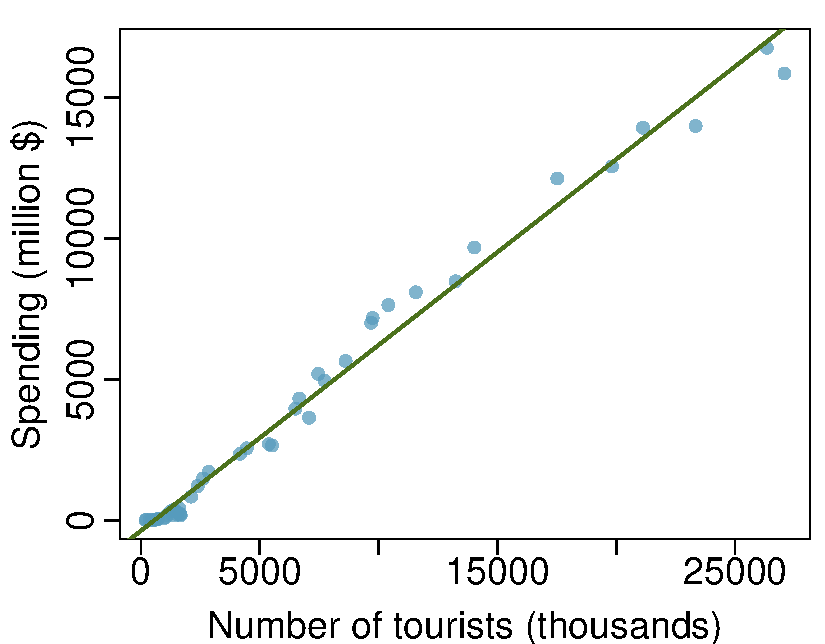
\includegraphics[width=0.32\textwidth]{ch_regr_simple_linear/figures/eoce/tourism_spending_reg_conds/tourism_spending_count.pdf}
\includegraphics[width=0.32\textwidth]{ch_regr_simple_linear/figures/eoce/tourism_spending_reg_conds/tourism_spending_count_residuals.pdf}
\includegraphics[width=0.32\textwidth]{ch_regr_simple_linear/figures/eoce/tourism_spending_reg_conds/tourism_spending_count_residuals_hist.pdf}
\end{center}
\begin{parts}
\item Describe the relationship between number of tourists and spending.
\item What are the explanatory and response variables?
\item Why might we want to fit a regression line to these data?
\item Do the data meet the conditions required for fitting a least squares 
line? In addition to the scatterplot, use the residual plot and histogram 
to answer this question. 
\end{parts}
}{}

\D{\newpage}

% 22 - starbucks_cals_carbos

\eoce{\qt{Nutrition at Starbucks, Part I\label{starbucks_cals_carbos}} 
The scatterplot below shows the relationship between the number of 
calories and amount of carbohydrates (in grams) Starbucks food menu 
items contain.\footfullcite{data:starbucksCals} Since Starbucks only 
lists the number of calories on the display items, we are interested 
in predicting the amount of carbs a menu item has based on its 
calorie content.
\begin{center}
\tabspecial{tableau-starbucks-p1}{
\includegraphics[width=0.32\textwidth]{ch_regr_simple_linear/figures/eoce/starbucks_cals_carbos/starbucks_cals_carbos.pdf}
\includegraphics[width=0.32\textwidth]{ch_regr_simple_linear/figures/eoce/starbucks_cals_carbos/starbucks_cals_carbos_residuals.pdf}
\includegraphics[width=0.32\textwidth]{ch_regr_simple_linear/figures/eoce/starbucks_cals_carbos/starbucks_cals_carbos_residuals_hist.pdf}}
\end{center}
\begin{parts}
\item Describe the relationship between number of calories and amount 
of carbohydrates (in grams) that Starbucks food menu items contain.
\item In this scenario, what are the explanatory and response 
variables?
\item Why might we want to fit a regression line to these data?
\item Do these data meet the conditions required for fitting a least 
squares line?
\end{parts}
}{}

% 23 - coast_starlight_reg_ahss

\eoce{\qt{The Coast Starlight, Part II\label{coast_starlight_reg_ahss}} \videosolution{ahss_eoce_sol-coast_starlight_reg} 
Exercise~\ref{coast_starlight_corr_units} introduces data on the Coast Starlight 
Amtrak train that runs from Seattle to Los Angeles. The mean travel 
time from one stop to the next on the Coast Starlight is 129 mins, 
with a standard deviation of 113 minutes. The mean distance traveled 
from one stop to the next is 108 miles with a standard deviation of 
99 miles. The correlation between travel time and distance is 0.636.
\begin{parts}
\item Write the equation of the regression line for predicting travel 
time.
\item Interpret the slope and the intercept in this context.
\item Calculate $R^2$ of the regression line for predicting travel 
time from distance traveled for the Coast Starlight, and interpret 
$R^2$ in the context of the application.
\item The distance between Santa Barbara and Los Angeles is 103 
miles. Use the model to estimate the time it takes for the Starlight 
to travel between these two cities.
\item It actually takes the Coast Starlight about 168 mins to travel 
from Santa Barbara to Los Angeles. Calculate the residual and explain 
the meaning of this residual value.
\item Suppose Amtrak is considering adding a stop to the Coast 
Starlight 500 miles away from Los Angeles. Would it be appropriate to 
use this linear model to predict the travel time from Los Angeles to 
this point? 
\end{parts}
}{}

% 24 - body_measurements_shoulder_height_reg_ahss

\eoce{\qt{Body measurements, Part III\label{body_measurements_shoulder_height_reg_ahss}}
Exercise~\ref{body_measurements_shoulder_height_corr_units} introduces 
data on shoulder girth and height of a group of individuals. The 
mean shoulder girth is 107.20 cm with a standard deviation of 
10.37 cm. The mean height is 171.14 cm with a standard deviation 
of 9.41 cm. The correlation between height and shoulder girth is 0.67.
\begin{parts}
\item Write the equation of the regression line for predicting height.
\item Interpret the slope and the intercept in this context.
\item Calculate $R^2$ of the regression line for predicting height 
from shoulder girth, and interpret it in the context of the 
application.
\item A randomly selected student from your class has a shoulder 
girth of 100 cm. Predict the height of this student using the model.
\item The student from part~(d) is 160 cm tall. Calculate the 
residual, and explain what this residual means.
\item A one year old has a shoulder girth of 56 cm. Would it be 
appropriate to use this linear model to predict the height of this 
child?
\end{parts}
}{}

\D{\newpage}

% 25 - murders_poverty_reg

\eoce{\qt{Murders and poverty, Part I\label{murders_poverty_reg}} \videosolution{ahss_eoce_sol-murders_poverty_reg} The following 
regression output is for predicting annual murders per million from 
percentage living in poverty in a random sample of 20 metropolitan 
areas.\\[2mm]
\begin{minipage}[c]{0.56\textwidth}
{\footnotesize
\begin{tabular}{rrrrr}
    \hline
            & Estimate  & Std. Error    & t value   & Pr($>$$|$t$|$) \\ 
    \hline
(Intercept) & -29.901   & 7.789         & -3.839    & 0.001 \\ 
poverty\%   & 2.559     & 0.390         & 6.562     & 0.000 \\ 
   \hline
\end{tabular}
$s = 5.512 \hfill R^2 = 70.52\% \hfill R^2_{adj} = 68.89\%$ 
}
\begin{parts}
\item Write out the linear model.
\item Interpret the intercept.
\item Interpret the slope.
\item Interpret $R^2$.
\item Calculate the correlation coefficient.
\end{parts}
\end{minipage}
\begin{minipage}[c]{0.02\textwidth}
$\:$\\
\end{minipage}
\begin{minipage}[c]{0.39\textwidth}
\includegraphics[width=\textwidth]{ch_regr_simple_linear/figures/eoce/murders_poverty_reg/murders_poverty.pdf}
\end{minipage}
}{}

% 26 - cat_body_heart_reg

\eoce{\qt{Cats, Part I\label{cat_body_heart_reg}} The following regression output is 
for predicting the heart weight (in g) of cats from their body weight 
(in kg). The coefficients are estimated using a dataset of 144 
domestic cats.\\[2mm]
\begin{minipage}[c]{0.56\textwidth}
{\footnotesize
\begin{tabular}{rrrrr}
    \hline
            & Estimate  & Std. Error    & t value   & Pr($>$$|$t$|$) \\ 
    \hline
(Intercept) & -0.357    & 0.692         & -0.515    & 0.607 \\ 
body wt     & 4.034     & 0.250         & 16.119    & 0.000 \\ 
    \hline
\end{tabular}
$s = 1.452 \hfill R^2 = 64.66\% \hfill R^2_{adj} = 64.41\%$ 
}
\begin{parts}
\item Write out the linear model.
\item Interpret the intercept.
\item Interpret the slope.
\item Interpret $R^2$.
\item Calculate the correlation coefficient.
\end{parts}
\end{minipage}
\begin{minipage}[c]{0.02\textwidth}
$\:$\\
\end{minipage}
\begin{minipage}[c]{0.39\textwidth}
\includegraphics[width=\textwidth]{ch_regr_simple_linear/figures/eoce/cat_body_heart_reg/cat_body_heart.pdf}
\end{minipage}
}{}

% 27 - outliers_1

\eoce{\qt{Outliers, Part I\label{outliers_1}} Identify the outliers in the 
scatterplots shown below, and determine what type of outliers they are. 
Explain your reasoning.
\begin{center}
\includegraphics[width=0.32\textwidth]{ch_regr_simple_linear/figures/eoce/outliers_1/outliers_1_influential.pdf}
\includegraphics[width=0.32\textwidth]{ch_regr_simple_linear/figures/eoce/outliers_1/outliers_2_leverage.pdf}
\includegraphics[width=0.32\textwidth]{ch_regr_simple_linear/figures/eoce/outliers_1/outliers_3_outlier.pdf}
\end{center}
}{}

\D{\newpage}

% 28 - outliers_2

\eoce{\qt{Outliers, Part II\label{outliers_2}} Identify the outliers in the scatterplots 
shown below and determine what type of outliers they are. Explain 
your reasoning.
\begin{center}
\includegraphics[width=0.32\textwidth]{ch_regr_simple_linear/figures/eoce/outliers_2/outliers_1_influential.pdf}
\includegraphics[width=0.32\textwidth]{ch_regr_simple_linear/figures/eoce/outliers_2/outliers_2_influential.pdf}
\includegraphics[width=0.32\textwidth]{ch_regr_simple_linear/figures/eoce/outliers_2/outliers_3_outlier.pdf}
\end{center}
}{}

% 29 - urban_homeowners_outlier

\eoce{\qt{Urban homeowners, Part I\label{urban_homeowners_outlier}} The 
scatterplot below shows the percent of families who own their 
home vs. the percent of the population living in urban areas.
\footfullcite{data:urbanOwner} There are 52 observations, each 
corresponding to a state in the US. Puerto Rico and District of 
Columbia are also included.

\noindent\begin{minipage}[c]{0.5\textwidth}
\begin{parts}
\item Describe the relationship between the percent of families who 
own their home and the percent of the population living in urban areas.
\item The outlier at the bottom right corner is District of Columbia, 
where 100\% of the population is considered urban. What type of an outlier 
is this observation?
\end{parts}
\end{minipage}
\begin{minipage}[c]{0.05\textwidth}
$\:$\\
\end{minipage}
\begin{minipage}[c]{0.4\textwidth}
\includegraphics[width=0.95\textwidth]{ch_regr_simple_linear/figures/eoce/urban_homeowners_outlier/urban_homeowners_outlier.pdf} \vspace{-3mm}
\end{minipage}
}{}

% 30 - crawling_babies_outlier

\eoce{\qt{Crawling babies, Part II\label{crawling_babies_outlier}} 
Exercise~\ref{crawling_babies_corr_units} introduces 
data on the average monthly temperature during the month babies first 
try to crawl (about 6 months after birth) and the average first 
crawling age for babies born in a given month. A scatterplot of these 
two variables reveals a potential outlying month when the average 
temperature is about 53\degree F and average crawling age is about 
28.5 weeks. Does this point have high leverage? Is it an influential 
point?
}{}
}






%__________________
\section[Inference for the slope of a regression line]{Inference for the slope of a regression line }
\label{inferenceForLinearRegression}

\sectionintro{
\noindent%
Here we encounter our last confidence interval and hypothesis test procedures, this time for making inferences about the slope of the population regression line.  We can use this to answer questions such as the following:
\begin{itemize}
\item Is the unemployment rate a significant linear predictor for the loss of the President's party in the House of Representatives?

\item On average, how much less in college gift aid do students receive when their parents earn an additional \$1000 in income? 
\end{itemize}


\subsection*{Learning objectives}
\begin{enumerate}
\setlength{\itemsep}{0mm}
\item Recognize that the slope of the sample regression line is a point estimate and has an associated standard error.

\item Be able to read the results of computer regression output and identify the quantities needed for inference for the slope of the regression line, specifically the slope of the sample regression line, the $SE$ of the slope, and the degrees of freedom.

\item State and verify whether or not the conditions are met for inference on the slope of the regression line based using the $t$-distribution.

\item Carry out a complete confidence interval procedure for the slope of the regression line.  


\item Carry out a complete hypothesis test for the slope of the regression line.

\item Distinguish between when to use the $t$-test for the slope of a regression line and when to use the matched pairs $t$-test for a mean of differences.
\end{enumerate}
}

\subsection{The role of inference for regression parameters}


Previously, we found the equation of the regression line for predicting gift aid from family income at Elmhurst College.  The slope, $b$, was equal to $-0.0431$.  This is the slope for our sample data.  However, the sample was taken from a larger population.   We would like to use the slope computed from our sample data to estimate the slope of the population regression line.

The equation for the population regression line can be written as
\begin{align*}
\mu_y = \alpha + \beta x
\end{align*}
Here, $\alpha$ and $\beta$ represent two model parameters\index{parameter}, namely the $y$-intercept and the slope of the true or population regression line. (This use of $\alpha$ and $\beta$\index{Greek!beta@beta ($\beta$)} have nothing to do with the $\alpha$ and $\beta$ we used previously to represent the probability of a Type~I Error and Type~II Error!) The parameters $\alpha$ and $\beta$ are estimated using data.  We can look at the equation of the regression line calculated from a particular data set:
\begin{align*}
\hat{y} =& a  + bx 
\end{align*}
and see that $a$ and $b$ are point estimates for $\alpha$ and $\beta$, respectively.  
If we plug in the values of $a$ and $b$, the regression equation for predicting gift aid based on family income is:
\begin{align*}
\hat{y}=24.3193-0.0431x
\end{align*}
The slope of the sample regression line, $-0.0431$, is our best estimate for the slope of the population regression line, but there is variability in this estimate since it is based on a sample.  A different sample would produce a somewhat different estimate of the slope.  The standard error of the slope tells us the typical variation in the slope of the sample regression line and the typical error in using this slope to estimate the slope of the population regression line.  

We would like to construct a 95\% confidence interval for $\beta$, the slope of the population regression line. As with means, inference for the slope of a regression line is based on the $t$-distribution.



\begin{onebox}
{Inference for the slope of a regression line}
Inference for the slope of a regression line is based on the $t$-distribution with $n-2$ degrees of freedom, where $n$ is the number of paired observations.
\end{onebox}

Once we verify that conditions for using the $t$-distribution are met, we will be able to construct the confidence interval for the slope using a critical value $t^{\star}$ based on $n-2$ degrees of freedom.  We will use a table of the regression summary to find the point estimate and standard error for the slope.


%%
\subsection{Conditions for the least squares line}

Conditions for inference in the context of regression can be more complicated than when dealing with means or proportions.  

Inference for parameters of a regression line involves the following assumptions:
\begin{description}
\setlength{\itemsep}{0mm}
\item[Linearity.] The true relationship between the two variables follows a linear trend.  We check whether this is reasonable by examining whether the data follows a linear trend.  If there is a nonlinear trend (e.g. left panel of Figure~\ref{whatCanGoWrongWithLinearModel}), an advanced regression method from another book or later course should be applied.
\item[Nearly normal residuals.] For each $x$-value, the residuals should be nearly normal.
When this assumption is found to be unreasonable, it is usually because of outliers or concerns about influential points.  An example which suggestions non-normal residuals is shown in the second panel of Figure~\ref{whatCanGoWrongWithLinearModel}.  If the sample size $n\ge 30$, then this assumption is not necessary.
\item[Constant variability.] The variability of points around the true least squares line is constant for all values of $x$. An example of non-constant variability is shown in the third panel of Figure~\ref{whatCanGoWrongWithLinearModel}.
\item[Independent.] The observations are independent of one other.  The observations can be considered independent when they are collected from a random sample or randomized experiment.  Be careful of data collected sequentially in what is called a \term{time series}.  An example of data collected in such a fashion is shown in the fourth panel of Figure~\ref{whatCanGoWrongWithLinearModel}.
\end{description}

\begin{figure}
\centering
\includegraphics[width=\textwidth]{ch_regr_simple_linear/figures/whatCanGoWrongWithLinearModel/whatCanGoWrongWithLinearModel}
\caption{Four examples showing when the inference methods in this chapter are insufficient to apply to the data. In the left panel, a straight line does not fit the data. In the second panel, there are outliers; two points on the left are relatively distant from the rest of the data, and one of these points is very far away from the line. In the third panel, the variability of the data around the line increases with larger values of $x$. In the last panel, a time series data set is shown, where successive observations are highly correlated.}
\label{whatCanGoWrongWithLinearModel}
\end{figure}

We see in Figure~\ref{whatCanGoWrongWithLinearModel}, that patterns in the residual plots suggest that the assumptions for regression inference are not met in those four examples.  In fact, identifying nonlinear trends in the data, outliers, and non-constant variability in the residuals are often easier to detect in a residual plot than in a scatterplot.  

We note that the second assumption regarding nearly normal residuals is particularly difficult to assess when the sample size is small.  We can make a graph, such as a histogram, of the residuals, but we cannot expect a small data set to be nearly normal.  All we can do is to look for excessive skew or outliers.  Outliers and influential points in the data can be seen from the residual plot as well as from a histogram of the residuals.

\begin{onebox}{Conditions for inference on the slope of a regression line}
\begin{enumerate}
\item The data is collected from a random sample or randomized experiment.
\item The residual plot appears as a random cloud of points and does not have any patterns or significant outliers that would suggest that the linearity, nearly normal residuals, constant variability, or independence assumptions are unreasonable.  
\end{enumerate}
\end{onebox} 

\subsection{Constructing a confidence interval for the slope of a regression line}

We would like to construct a confidence interval for the slope of the regression line for predicting gift aid based on family income for \emph{all} freshmen at Elmhurst college.  



Do conditions seem to be satisfied?  We recall that the 50 freshmen in the sample were randomly chosen, so the observations are independent.  Next, we need to look carefully at the scatterplot and the residual plot.  


\begin{onebox}{Always check conditions}
Do not blindly apply formulas or rely on regression output; always first look at a scatterplot or a residual plot.  If conditions for fitting the regression line are not met, the methods presented here should not be applied. 
\end{onebox}

The scatterplot seems to show a linear trend, which matches the fact that there is no curved trend apparent in the residual plot.  Also, the standard deviation of the residuals is mostly constant for different $x$ values and there are no outliers or influential points.  There are no patterns in the residual plot that would suggest that a linear model is not appropriate, so the conditions are reasonably met.  We are now ready to calculate the 95\% confidence interval.  

\begin{figure}%
   \centering
  \begin{tabular}{cc}
   \includegraphics[width=0.5\textwidth]{ch_regr_simple_linear/figures/elmhurstInference/elmhurstScatter}
   \includegraphics[width=0.5\textwidth]{ch_regr_simple_linear/figures/elmhurstInference/elmhurstResidual}
\end{tabular}
   \caption{Left: Scatterplot of gift aid versus family income for 50 freshmen at Elmhurst college.  Right: Residual plot for the model shown in left panel.  }
\label{elmhurstInferencePlots}
\end{figure}




\begin{figure}[ht]
\centering
\begin{tabular}{l rrrr}
  \hline
  \vspace{-3.7mm} & & & & \\
 & Estimate & Std. Error & t value & Pr($>$$|$t$|$) \\ 
  \hline
  \vspace{-3.6mm} & & & & \\
(Intercept) & 24.3193 & 1.2915 & 18.83 & 0.0000 \\ 
family\us{}income & -0.0431 & 0.0108 & -3.98 & 0.0002 \\ 
  \hline
\end{tabular}
\caption{Summary of least squares fit for the Elmhurst College data, where we are predicting gift aid by the university based on the family income of students.}
\label{rOutputForIncomeAidLSRLine2}
\end{figure}


\begin{examplewrap}
\begin{nexample}
{Construct a 95\% confidence interval for the slope of the regression line for predicting gift aid from family income at Elmhurst college.  }
As usual, the confidence interval will take the form:  
\begin{align*}
\text{point estimate} \pm \text{critical value}\times SE \text{ of estimate}
\end{align*}
The point estimate for the slope of the population regression line is the slope of the sample regression line:  $-0.0431$.  The standard error of the slope can be read from the table as 0.0108.  Note that we do not need to divide 0.0108 by the square root of $n$ or do any further calculations on 0.0108; 0.0108 \emph{is} the $SE$ of the slope.  Note that the value of $t$ given in the table refers to the test statistic, not to the critical value $t^{\star}$.  To find $t^{\star}$ we can use a $t$-table. Here $n=50$, so $df=50-2=48$.  Using a $t$-table, we round down to row $df=40$ and we estimate the critical value $t^{\star}=2.021$ for a 95\% confidence level.  The confidence interval is calculated as:
\begin{align*}
-0.0431 \ \pm \ & 2.021\times 0.0108\\
=(-0.06&5, -0.021 )
\end{align*}
Note: $t^{\star}$ using exactly 48 degrees of freedom is equal to 2.01 and gives the same interval of $(-0.065,\ -0.021)$.
\end{nexample}
\end{examplewrap}


\begin{examplewrap}
\begin{nexample}
{Intepret the confidence interval in context.  What can we conclude?}
We are 95\% confident that the slope of the population regression line, the true average change in gift aid for each additional \$1000 in family income, is between $-\$0.065$ thousand dollars and $-\$0.021$ thousand dollars.  That~is, we are 95\% confident that, on average, when family income is \$1000 higher, gift aid is between \$21 and \$65 \emph{lower}.  

Because the entire interval is negative, we have evidence that the slope of the population regression line is less than 0.  In other words, we have evidence that there is a significant negative linear relationship between gift aid and family income.
\end{nexample}
\end{examplewrap}

\begin{onebox}{Constructing a confidence interval for the slope of regression line}
To carry out a complete confidence interval procedure to estimate the slope of the population regression line $\beta$ of a regression line,
\\
\\
\inferencestep{Identify} Identify the parameter and the confidence level, C\%.\vspace{-1mm}
\begin{itemize} 
\item[] The parameter will be a slope of the population regression line, e.g. the slope of the population regression line relating air quality index to average rainfall per year for each city in the United States.  
\end{itemize}
\inferencestep{Choose} Choose the correct interval procedure and identify it by name. \vspace{-1mm}
\begin{itemize}
\item[] Here we use choose the \termsub{$\pmb{t}$-interval for the slope}{t-interval for the slope@$t$-interval for the slope}.
\end{itemize}
\inferencestep{Check} Check conditions for using a $t$-interval for the slope.\vspace{-1mm}
\begin{itemize}
\setlength{\itemsep}{0mm}
\item[] 1.  Data come from a random sample or randomized experiment.
\item[] 2.  The residual plot shows no pattern implying that a linear model is reasonable. \item[] \quad \ More specifically, the residuals should be independent, nearly normal (or $n\ge 30$),
\item [] \quad \  and have constant standard deviation.
\end{itemize}
\inferencestep{Calculate} Calculate the confidence interval and record it in interval form.
\begin{itemize}
\item[] $\text{point estimate}\ \pm\ t^{\star} \times SE\ \text{of estimate}$, \quad $df = n - 2$
\begin{itemize}											
\item[] point estimate: the slope $b$ of the sample regression line
\item[] $SE$ of estimate: $SE$ of slope (find using computer output)
\item[] $t^{\star}$: use a $t$-distribution with $df = n-2$ and confidence level C\%
\end{itemize}
\item[] (\underline{\ \ \ \ \ }, \underline{\ \ \ \ \ })
\end{itemize}
\inferencestep{Conclude}  Interpret the interval and, if applicable, draw a conclusion in context.\vspace{-1mm}
\begin{itemize}
\item[] We are C\%  confident that the true \emph{slope} of the regression line, the average change in [y] for each unit increase in [x], is between \underline{\ \ \ \ \ } and \underline{\ \ \ \ \ }. If applicable, draw a conclusion based on whether the interval is entirely above, is entirely below, or contains the value 0. 
\end{itemize}
\end{onebox}

\begin{figure}%
   \centering
  \begin{tabular}{cc}
   \includegraphics[width=0.5\textwidth]{ch_regr_simple_linear/figures/possumInference/possumScatter}
   \includegraphics[width=0.5\textwidth]{ch_regr_simple_linear/figures/possumInference/possumResidual}
\end{tabular}
   \caption{Left: Scatterplot of head length versus total length for 104 brushtail possums.   Right: Residual plot for the model shown in left panel.  }
\label{possumInferencePlots}
\end{figure}

\begin{examplewrap}
\begin{nexample}{


The regression summary below shows statistical software output from fitting the least squares regression line for predicting head length from total length for 104 brushtail possums.  The scatterplot and residual plot are shown above. 
\\
\\
\texttt{Predictor \ \ \ \ \ \ \ Coef \ \ \ \ \ \ \ SE Coef \ \ T \ \ \ \ \ \ \ P} \\
\texttt{Constant \ \ \ \ \ \ \ \  42.70979 \ \ \ 5.17281 \ \ 8.257 \ \ 5.66e-13} \\
\texttt{total\us{}length\ \ \ \ \ \ 0.57290 \ \ \ 0.05933 \ \ 9.657 \ \ 4.68e-16} \\

\texttt{S = 2.595\ \ \ \ R-Sq = 47.76\% \ \ \ R-Sq(adj) = 47.25\%}
%\label{rOutputForPossum}
\\
\\
Construct a 95\% confidence interval for the slope of the regression line.  Is there convincing evidence that there is a positive, linear relationship between head length and total length? Use the five step framework to organize your work.}
\begin{description}
\item[\inferencestep{Identify}] The parameter of interest is the slope of the population regression line for predicting head length from body length.  We want to estimate this at the 95\% confidence level.  
\item[\inferencestep{Choose}] Because the parameter to be estimated is the slope of a regression line, we will use the $t$-interval for the slope.
\item[\inferencestep{Check}] These data come from a random sample.  The residual plot shows no pattern.  In general, the residuals have constant standard deviation and there are no outliers or influential points.  Also $n=104\ge 30$ so some skew in the residuals would be acceptable. A linear model is reasonable here.
\item[\inferencestep{Calculate}]  We will calculate the interval:
$\text{point estimate}\ \pm\ t^{\star} \times SE\ \text{of estimate}$

We read the slope of the sample regression line and the corresponding $SE$ from the table.  The point estimate is $b = 0.57290$.  The $SE$ of the slope is 0.05933, which can be found next to the slope of 0.57290.  The degrees of freedom is $df=n-2=104-2=102$.  As before, we find the critical value $t^{\star}$ using a $t$-table (the $t^{\star}$ value is not the same as the $T$-statistic for the hypothesis test).   Using the $t$-table at row $df = 100$ (round down since 102 is not on the table) and confidence level 95\%, we get $t^{\star}=1.984$.  
\\
\\
So the 95\% confidence interval is given by:
\begin{align*}
0.57290 \ \pm\  &1.984\times  0.05933\\
 (0.456&, 0.691)
\end{align*}
\item[\inferencestep{Conclude}]  We are 95\% confident that the slope of the population regression line is between 0.456 and 0.691.  That is, we are 95\% confident that the true average \emph{increase} in head length for each additional~cm in total length is between 0.456~mm and 0.691~mm.  Because the interval is entirely above 0, we do have evidence of a positive linear association between the head length and body length for brushtail possums.  
\end{description}


\end{nexample}
\end{examplewrap}



\D{\newpage}

%%
\subsection[Calculator: the $t$-interval for the slope]{Calculator: the linear regression \pmb{$t$}-interval for the slope}
We will rely on regression output from statistical software when constructing confidence intervals for the slope of a regression line.  We include calculator instructions here simply for completion.

\begin{onebox}{\videohref{ti84_regression_t_confint} TI-84: T-interval for \pmb{$\beta$}}
\label{LinRegint}
Use \calctext{STAT}, \calctext{TESTS}, \calctext{LinRegTInt}.
\begin{enumerate}
\setlength{\itemsep}{0mm}
\item Choose \calctext{STAT}.
\item Right arrow to \calctext{TESTS}.
\item Down arrow and choose \calctext{G:} \calctext{LinRegTInt}.\vspace{-1.5mm}
  \begin{itemize}
  \item This test is not built into the TI-83.
  \end{itemize}
\item Let \calctext{Xlist} be \calctext{L1} and \calctext{Ylist} be \calctext{L2}. (Don't forget to enter the $x$ and $y$ values in \calctext{L1} and \calctext{L2} before doing this interval.)
\item Let \calctext{Freq} be \calctext{1}.
\item Enter the desired confidence level.
\item Leave \calctext{RegEQ} blank.
\item Choose \calctext{Calculate} and hit \calcbutton{ENTER}, which returns: \\[1mm]
\begin{tabular}{l l}
\calctext{(\underline{\ \ },\underline{\ \ })} & the confidence interval \\
\calctext{b} & $b$, the slope of best fit line of the sample data \\
\calctext{df} &degrees of freedom associated with this confidence interval \\
\calctext{s} & standard deviation of the residuals (not the same as $SE$ of the slope) \\
\calctext{a} & $a$, the y-intercept of the best fit line of the sample data \\
$\calctextmath{r^2}$ & $R^2$, the explained variance \\
\calctext{r} & $r$, the correlation coefficient \\
\end{tabular}
\end{enumerate}
\end{onebox}




%%
\subsection{Midterm elections and unemployment}

\index{data!midterm elections|(}

Elections for members of the United States House of Representatives occur every two years, coinciding every four years with the U.S. Presidential election. The set of House elections occurring during the middle of a Presidential term are called \indexthis{midterm elections}{midterm election}. In America's two-party system, one political theory suggests the higher the unemployment rate, the worse the President's party will do in the midterm elections.

To assess the validity of this claim, we can compile historical data and look for a connection. We consider every midterm election from 1898 to 2018, with the exception of those elections during the Great Depression. Figure~\ref{unemploymentAndChangeInHouse} shows these data and the least-squares regression line: \vspace{-2mm}
\begin{align*}
&\text{\% change in House seats for President's party}  \\
&\qquad\qquad= -7.36 - 0.89\times \text{(unemployment rate)}
\end{align*}
We consider the percent change in the number of seats of the President's party (e.g. percent change in the number of seats for Republicans in 2018) against the unemployment rate.

Examining the data, there are no clear deviations from linearity, the constant variance condition, or the normality of residuals. While the data are collected sequentially, a separate analysis was used to check for any apparent correlation between successive observations; no such correlation was found.

\begin{figure}[h]
\centering
\oiRedirect{tableau-scatter-changeinseats-unemployment}{\includegraphics[width=.9\textwidth]{ch_regr_simple_linear/figures/unemploymentAndChangeInHouse/unemploymentAndChangeInHouse}}
\caption{The percent change in House seats for the President's party in each election from 1898 to 2018 plotted against the unemployment rate. The two points for the Great Depression have been removed, and a least squares regression line has been fit to the data.  Explore this data set on Tableau Public\tableauhref{tableau-scatter-changeinseats-unemployment}.}
\label{unemploymentAndChangeInHouse}
\end{figure}

\D{\newpage}

\begin{exercisewrap}
\begin{nexercise}
The data for the Great Depression (1934 and 1938) were removed because the unemployment rate was 21\% and 18\%, respectively. Do you agree that they should be removed for this investigation? Why or why not?\footnotemark 
\end{nexercise}
\end{exercisewrap}
\footnotetext{We will provide two considerations. Each of these points would have very high leverage on any least-squares regression line, and years with such high unemployment may not help us understand what would happen in other years where the unemployment is only modestly high. On the other hand, these are exceptional cases, and we would be discarding important information if we exclude them from a final analysis.}

There is a negative slope in the line shown in Figure~\ref{unemploymentAndChangeInHouse}. However, this slope (and the y-intercept) are only estimates of the parameter values. We might wonder, is this convincing evidence that the ``true'' linear model has a negative slope? That is, do the data provide strong evidence that the political theory is accurate?  We can frame this investigation as a statistical hypothesis test:
\begin{itemize}
\item[$H_0$:] $\beta = 0$. The true linear model has slope zero.
\item[$H_A$:] $\beta < 0$. The true linear model has a slope less than zero. The higher the unemployment, the greater the loss for the President's party in the House of Representatives.
\end{itemize}
We would reject $H_0$ in favor of $H_A$ if the data provide strong evidence that the slope of the population regression line is less than zero. To assess the hypotheses, we identify a standard error for the estimate, compute an appropriate test statistic, and identify the p-value.
Before we calculate these quantities, how good are we at visually determining from a scatterplot when a slope is significantly less than or greater than 0?  And why do we tend to use a 0.05 significance level as our cutoff?  Try out the following activity which will help answer these questions.

\begin{onebox}{Testing for the slope using a cutoff of 0.05}
  What does it mean to say that the slope of the population regression line is significantly greater than 0?  And why do we tend to use a cutoff of $\alpha = 0.05$?   
  This 5-minute interactive task will explain: 
  \begin{center}
  \oiRedirect{textbook-why05}{www.openintro.org/why05}
  \end{center}
\end{onebox}


\D{\newpage}

%%
\subsection{Understanding regression output from software}
\label{testStatisticForTheSlope}

The residual plot shown in Figure~\ref{unemploymentAndChangeInHouseResiduals} shows no pattern that would indicate that a linear model is inappropriate.  Therefore we can carry out a test on the population slope using the sample slope as our point estimate.  Just as for other point estimates we have seen before, we can compute a standard error and test statistic for $b$. The test statistic $T$ follows a $t$-distribution with $n-2$ degrees of freedom.

\begin{figure}[h]
\centering
\oiRedirect{tableau-residuals-changeinsets-unemployment}{\includegraphics[width=.9\textwidth]{ch_regr_simple_linear/figures/unemploymentAndChangeInHouse/unemploymentAndChangeInHouseResiduals}}
\caption{The residual plot shows no pattern that would indicate that a linear model is inappropriate.  Explore this data set on Tableau Public\tableauhref{tableau-residuals-changeinsets-unemployment}.}
\label{unemploymentAndChangeInHouseResiduals}
\end{figure}

\begin{onebox}{Hypothesis tests on the slope of the regression line}
Use a $t$-test with $n - 2$ degrees of freedom when performing a hypothesis test on the slope of a regression line.\end{onebox}


We will rely on statistical software to compute the standard error and leave the explanation of how this standard error is determined to a second or third statistics course.
Figure~\ref{midtermElectionUnemploymentRRegressionOutput} shows software output for the least squares regression line in Figure~\ref{unemploymentAndChangeInHouse}. The row labeled \emph{unemp} represents the information for the slope, which is the coefficient of the unemployment variable.


\begin{figure}[h]
\centering
\begin{tabular}{rrrrr}
  \hline
  \vspace{-3.7mm} & & & & \\
 & Estimate & Std. Error & t value & Pr($>$$|$t$|$) \\ 
  \hline
  \vspace{-3.6mm} & & & & \\
(Intercept) & -7.3644  & 5.1553 & -1.43 & 0.1646\\ 
unemp & -0.8897 & 0.8350 & -1.07 & 0.2961 \\ 
   \hline
\end{tabular}
\caption{Least squares regression summary for the percent change in seats of president's party in House of Reprepsentatives based on percent unemployment.}
\label{midtermElectionUnemploymentRRegressionOutput}
\end{figure}




\begin{examplewrap}
\begin{nexample}{What do the first column of numbers in the regression summary represent?}
The entries in the first column represent the least squares estimates for the $y$-intercept and slope, $a$ and $b$ respectively.  Using this information, we could write the equation
  for the least squares regression line as
  \begin{align*}
  \hat{y} = -7.3644 - 0.8897 x
  \end{align*}
  where $y$ in this case represents the percent change in the number
  of seats for the president's party,
  and $x$ represents the unemployment rate.
\end{nexample}
\end{examplewrap}

We previously used a test statistic $T$ for hypothesis testing in the context of means. Regression is very similar. Here, the point estimate is $b=-0.8897$.  The $SE$ of the estimate is 0.8350, which is given in the second column, next to the estimate of $b$.  This $SE$ represents the typical error when using the slope of the sample regression line to estimate the slope of the population regression line.

The null value for the slope is 0, so we now have everything we need to compute the test statistic.  We have: 
\begin{align*}
T = \frac{\text{point estimate} - \text{null value}}{SE \text{ of estimate}} = \frac{-0.8897 - 0}{0.8350} = -1.07
\end{align*}
This value corresponds to the $T$-score reported in the regression output in the third column along the \emph{unemp} row.  

\begin{figure}
\centering
\includegraphics[width=0.82\textwidth]{ch_regr_simple_linear/figures/oneSidedTailForMidtermUnemploymentHT/oneSidedTailForMidtermUnemploymentHT}
\caption{The distribution shown here is the sampling distribution for $b$, if the null hypothesis was true. The shaded tail represents the p-value for the hypothesis test evaluating whether there is convincing evidence that higher unemployment corresponds to a greater loss of House seats for the President's party during a midterm election.}
\label{oneSidedTailForMidtermUnemploymentHT}
\end{figure}

\begin{examplewrap}
\begin{nexample}{In this example, the sample size $n=27$. Identify the degrees of freedom and p-value for the hypothesis test.}
The degrees of freedom for this test is $n-2$, or $df = 27-2 = 25$. We could use a table or a calculator to find the probability of a value less than -1.07 under the $t$-distribution with 25 degrees of freedom.  However, the two-side p-value is given in Figure~\ref{midtermElectionUnemploymentRRegressionOutput}, next to the corresponding $t$-statistic.  Because we have a one-sided alternate hypothesis, we take half of this.  The p-value for the test is $\frac{0.2961}{2}=0.148$.  
\index{data!midterm elections|)}
\end{nexample}
\end{examplewrap}

\D{\newpage}

Because the p-value is so large, we do not reject the null hypothesis. That is, the data do not provide convincing evidence that a higher unemployment rate is associated with a larger loss for the President's party in the House of Representatives in midterm elections.


\begin{onebox}{Don't carelessly use the p-value from regression output}
{The last column in regression output often lists p-values for one particular hypothesis: a two-sided test where the null value is zero. If your test is one-sided and the point estimate is in the direction of $H_A$, then you can halve the software's p-value to get the one-tail area. If neither of these scenarios match your hypothesis test, be cautious about using the software output to obtain the p-value.}
\end{onebox}




%%

\begin{onebox}{Hypothesis test for the slope of regression line}
To carry out a complete hypothesis test for the claim that there is no linear relationship between two numerical variables, i.e. that $\beta=0$, 
\\
\\
\inferencestep{Identify} Identify the hypotheses and the significance level, $\alpha$.\vspace{-1mm}
\begin{itemize}
\setlength{\itemsep}{0mm}
\item[] $H_0$: $\beta = 0$  
\item[]  $H_A$: $\beta \ne 0$;  \quad $H_A$: $\beta > 0$; \quad or \quad $H_A$: $\beta < 0$ 
\end{itemize} 
\inferencestep{Choose} Choose the correct test procedure and identify it by name. \vspace{-1mm}
\begin{itemize}
\item[] Here we choose the \termsub{$\pmb{t}$-test for the slope}{t-test for the slope@$t$-test for the slope}. 
\end{itemize}
 \inferencestep{Check} Check conditions for using a $t$-test for the slope.\vspace{-1mm}
\begin{itemize}
\setlength{\itemsep}{0mm}
\item[] 1.  Data come from a random sample or randomized experiment.
\item[] 2.  The residual plot shows no pattern implying that a linear model is reasonable. \item[] \quad \ More specifically, the residuals should be independent, nearly normal (or $n\ge 30$),
\item [] \quad \  and have constant standard deviation.
\end{itemize}
 \inferencestep{Calculate}  Calculate the $t$-statistic, $df$, and p-value.
\begin{itemize}
\item[] $T= \frac{\text{point estimate } - \text{ null value}}{SE \text{ of estimate}}$, \quad $df=n-2$
\begin{itemize}
\item[] point estimate: the slope $b$ of the sample regression line
\item[] $SE$ of estimate:  $SE$ of slope (find using computer output)
\item[] null value: 0
\end{itemize}
\item[] p-value = (based on the $t$-statistic, the $df$, and the direction of $H_A$)
\end{itemize}
 \inferencestep{Conclude} Compare the p-value to $\alpha$, and draw a conclusion in context. \vspace{-1mm}
\begin{itemize}
\item[] If the p-value is $< \alpha$, reject $H_0$; there is sufficient evidence that [$H_A$ in context]. 
\item[] If the p-value is $> \alpha$, do not reject $H_0$; there is not sufficient evidence that [$H_A$ in context].
\end{itemize}\end{onebox}


\begin{examplewrap}
\begin{nexample}{
The regression summary below shows statistical software output from fitting the least squares regression line for predicting gift aid based on family income for 50 freshman students at Elmhurst College.  The scatterplot and residual plot were shown in Figure~\ref{elmhurstInferencePlots}. 
\\
\\
\texttt{Predictor \ \ \ \ \ \ \ Coef \ \ \ \ \ \ \ SE Coef \ \ T \ \ \ \ \ \ \ P} \\
\texttt{Constant \ \ \ \ \ \ \ \  24.31933 \ \ \ 1.29145 \ \ 18.831 \ \ < 2e-16} \\
\texttt{family\_income\ \ \ \ -0.04307 \ \ \ 0.01081 \ \ -3.985 \ \ 0.000229} \\

\texttt{S = 4.783\ \ \ \ R-Sq = 24.86\% \ \ \ R-Sq(adj) = 23.29\%}
%\label{rOutputForIncomeAidLSRLineInInferenceSection}
\\
\\
Do these data provide convincing evidence that there is a negative, linear relationship between family income and gift aid?  Carry out a complete hypothesis test at the 0.05 significance level.  Use the five step framework to organize your work.}

\begin{description}
\item[\inferencestep{Identify}]  We will test the following hypotheses at the $\alpha=0.05$ significance level.\\
$H_0$: $\beta = 0$. There is no linear relationship.\\
$H_A$: $\beta < 0$. There is a negative linear relationship.  
\\
\\
Here, $\beta$ is the slope of the population regression line for predicting gift aid from family income at Elmhurst College.
\item[\inferencestep{Choose}] Because the hypotheses are about the slope of a regression line, we choose the $t$-test for a slope.  
\item[\inferencestep{Check}]  The data come from a random sample.  Also, the residual plot shows that the residuals have constant variance and no outliers or influential points (and $n=50\ge 30$).  The lack of any pattern in the residual plot indicates that a linear model is appropriate.
\item[\inferencestep{Calculate}]  We will calculate the $t$-statistic, degrees of freedom, and the p-value.
\begin{align*}
T = \frac{\text{point estimate } - \text{ null value}}{SE \text{ of estimate}}
\end{align*}
We read the slope of the sample regression line and the corresponding $SE$ from the table.
\\
The point estimate is: $b = -0.04307$.
\\
The $SE$ of the slope is: $SE = 0.01081$.  
\begin{align*}
T = \frac{-0.04307 - 0}{0.01081} = -3.985
\end{align*}
Because $H_A$ uses a less than sign ($<$), meaning that it is a lower-tail test, the \mbox{p-value} is the area to the \emph{left} of $t=-3.985$ under the $t$-distribution with $50-2=48$ degrees of freedom.  The p-value = $\frac{1}{2}(0.000229)\approx 0.0001$.  
\item[\inferencestep{Conclude}]  The p-value of 0.0001 is $< 0.05$, so we reject $H_0$; there is sufficient evidence that there is a negative linear relationship between family income and gift aid at Elmhurst College.  
\end{description}



\end{nexample}
\end{examplewrap}
\label{overallAidIncomeInformalAssessmentOfRegressionLineSlope}




\D{\newpage}

%%
\subsection[Calculator: the $t$-test for the slope]{Calculator: the \pmb{$t$}-test for the slope}

When performing this type of inference, we generally make use of regression output that provides us with the necessary quantities: $b$ and $SE \text{ of } {b}$.  The calculator functions below require knowing all of the data and are, therefore, rarely used.  We describe them here for the sake of completion. 

\begin{onebox}{\videohref{ti84_regression_t_test} TI-83/84: Linear regression T-test on \pmb{$\beta$}}
\label{LinRegtest}
Use \calctext{STAT}, \calctext{TESTS}, \calctext{LinRegTTest}.
\begin{enumerate}
\setlength{\itemsep}{0mm}
\item Choose \calctext{STAT}.
\item Right arrow to \calctext{TESTS}.
\item Down arrow and choose \calctext{F:LinRegTTest}. (On TI-83 it is \calctext{E:LinRegTTest}).
\item Let \calctext{Xlist} be \calctext{L1} and \calctext{Ylist} be \calctext{L2}. (Don't forget to enter the $x$ and $y$ values in \calctext{L1} and \calctext{L2} before doing this test.)
\item Let \calctext{Freq} be \calctext{1}.
\item Choose $\calctextmath{\ne}$, $\calctextmath{<}$, or $\calctextmath{>}$ to correspond to $H_A$.
\item Leave \calctext{RegEQ} blank.
\item Choose \calctext{Calculate} and hit \calcbutton{ENTER}, which returns: \\[1mm]
\begin{tabular}{ll l ll}
\calctext{t} & t statistic &\quad&
	\calctext{b} & $b$, slope of the line \\
\calctext{p} & p-value &&
	\calctext{s} & st.~dev.~of the residuals \\
\calctext{df} & degrees of freedom for the test &&
	$\calctextmath{r^2}$ & $R^2$, explained variance \\
\calctext{a} & $a$, y-intercept of the line &&
	\calctext{r} & $r$, correlation coefficient
\end{tabular}
\end{enumerate}
\end{onebox} 

\begin{onebox}{\videohref{casio_regression_t_test} Casio fx-9750GII: Linear regression T-test on \pmb{$\beta$}}
\begin{enumerate}
\setlength{\itemsep}{0mm}
\item Navigate to \calctext{STAT} (\calcbutton{MENU} button, then hit the \calcbutton{2} button or select \calctext{STAT}).
\item Enter your data into 2 lists.
\item Select \calctext{TEST} (\calcbutton{F3}), \calctext{t} (\calcbutton{F2}), and \calctext{REG} (\calcbutton{F3}).
\item If needed, update the sidedness of the test and the \calctext{XList} and \calctext{YList} lists. The \calctext{Freq} should be set to \calctext{1}.
\item Hit \calcbutton{EXE}, which returns: \\[1mm]
\begin{tabular}{ll l ll}
\calctext{t} & t statistic &\quad&
	\calctext{b} & $b$, slope of the line \\
\calctext{p} & p-value &&
	\calctext{s} & st.~dev.~of the residuals \\
\calctext{df} & degrees of freedom for the test &&
	\calctext{r} & $r$, correlation coefficient \\
\calctext{a} & $a$, y-intercept of the line &&
	$\calctextmath{r^2}$ & $R^2$, explained variance
\end{tabular}
\end{enumerate}
\end{onebox} 

\begin{examplewrap}
\begin{nexample}
{Why does the calculator test include the symbol $\rho$ when choosing the direction of the alternate hypothesis?}
Recall the we used the letter $r$ to represent correlation.  The Greek letter $\rho=0$ represents the correlation for the entire population.  The slope $b=r\frac{s_y}{s_x}$.  If the slope of the population regression line is zero, the correlation for the population must also be zero.  For this reason, the $t$-test for $\beta=0$ is equivalent to a test for $\rho=0$.
\end{nexample}
\end{examplewrap}



\D{\newpage}

%%
\subsection{Which inference procedure to use for paired data?}

In Section~\ref{ciMeanOfDifferences}, we looked at a set of paired data involving the price of textbooks for UCLA courses at the UCLA Bookstore and on Amazon.  The left panel of Figure~\ref{textbooksHistogramScatter} shows the difference in price (UCLA Bookstore $-$ Amazon) for each book.   Because we have two data points on each textbook, it also makes sense to construct a scatterplot, as seen in the right panel of Figure~\ref{textbooksHistogramScatter}.

\begin{figure}[h]
\centering
\begin{tabular}{cc}
\includegraphics[width=0.55\textwidth]{ch_inference_for_means/figures/textbooksF18/diffInTextbookPricesF18}
\includegraphics[width=0.45\textwidth]{ch_regr_simple_linear/figures/textbooks_scatter/textbooks_scatter}
\end{tabular}
\caption{Left: histogram of the difference (UCLA Bookstore - Amazon) in price for
    each book sampled.  Right: scatterplot of Amazon Price versus UCLA Bookstore price.}
\label{textbooksHistogramScatter}
\end{figure}


\begin{examplewrap}
\begin{nexample}
{What additional information does the scatterplot provide about the price of textbooks at UCLA Bookstore and on Amazon?}With a scatterplot, we see the \emph{relationship} between the variables.  We can see when UCLA Bookstore price is larger, whether Amazon price tends to be larger.  We can consider the strength of the correlation and we can plot the linear regression equation.  
\end{nexample}
\end{examplewrap}

\begin{examplewrap}
\begin{nexample}
{Which test should we do if we want to check whether:
\begin{enumerate}
\item prices for textbooks for UCLA courses are \emph{higher} at the UCLA Bookstore than on Amazon
\item there is a significant, positive linear relationship between UCLA Bookstore price and Amazon price?
\end{enumerate}}
In the first case, we are interested in whether the differences (UCLA Bookstore $-$ Amazon) are, on average, greater than 0, so we would do a matched pairs $t$-test for a mean of differences.  In the second case, we are interested in whether the slope is significantly greater than 0, so we would do a $t$-test for the slope of a regression line.  
\end{nexample}
\end{examplewrap}

Likewise, a matched pairs $t$-interval for a mean of differences would provide an interval of reasonable values for mean of the differences for all UCLA textbooks, whereas a $t$-interval for the slope would provide an interval of reasonable values for the slope of the regression line for all UCLA textbooks.     


\begin{onebox}{Inference for paired data}
A matched pairs $t$-interval or $t$-test for a mean of differences only makes sense when we are asking whether, on average, one variable is \emph{greater} than another (think histogram of the differences).  A $t$-interval or $t$-test for the slope of a regression line makes sense when we are interested in the linear relationship between them (think scatterplot).  
\end{onebox}


\begin{examplewrap}
\begin{nexample}
{Previously, we looked at the relationship betweeen body length and head length for bushtail possums.  We also looked at the relationship between gift aid and family income for freshmen at Elmhurst College.  Could we do a matched pairs $t$-test in either of these scenarios?}
We have to ask ourselves, does it make sense to ask whether, on average, body length is greater than head length?  Similarly, does it make sense to ask whether, on average, gift aid is greater than family income?  These don't seem to be meaningful research questions; a matched pairs $t$-test for a mean of differences would not be useful here. 
\end{nexample}
\end{examplewrap}

\begin{exercisewrap}
\begin{nexercise}
A teacher gives her class a pretest and a posttest.  Does this result in paired data?  If so, which hypothesis test should she use?\footnotemark
\end{nexercise}
\end{exercisewrap}
\footnotetext{Yes, there are two observations for each individual, so there is paired data.  The appropriate test depends upon the question she wants to ask.  If she is interested in whether, on average, students do better on the posttest than the pretest, should use a matched pairs $t$-test for a mean of differences.  If she is interested in whether pretest score is a significant linear predictor of posttest score, she should do a $t$-test for the slope.  In this situation, both tests could be useful, but which one should be used is dependent on the teacher's research question.}


\D{\newpage}

%%
\subsection*{Section summary}

\noindent In Chapter 6, we used a $\chi^2$ test of independence to test for association between two categorical variables.  In this section, we test for association/correlation between two numerical variables.
\begin{itemize}
\item We use the slope $b$ as a \emph{point estimate} for the slope $\beta$ of the population regression line.  The slope of the population regression line is the true increase/decrease in $y$ for each unit increase in $x$.  If the slope of the population regression line is 0, there is no linear relationship between the two variables.  
\item Under certain assumptions, the sampling distribution of $b$ is \emph{normal} and the distribution of the standardized test statistic using the standard error of the slope follows a $\pmb{t}$\textbf{-distribution} with $n-2$ degrees of freedom.

\item When there is $(x, y)$ data and the parameter of interest is the slope of the population regression line, e.g. the slope of the population regression line relating air quality index to average rainfall per year for each city in the United States:
\begin{itemize}
\item Estimate $\beta$ at the C\% confidence level using a \termsub{$\pmb{t}$-interval for the slope}{t-interval for the slope@$t$-interval for the slope}.
\item Test $H_0$: $\beta=0$ at the $\alpha$ significance level using a \termsub{$\pmb{t}$-test for the slope}{t-test for the slope@$t$-test for the slope}.
\end{itemize}
\item The conditions for the $t$-interval and $t$-test for the slope of a regression line are the same.
\begin{itemize}
\setlength{\itemsep}{0mm}
\item[1.] Data come from a random sample or randomized experiment.
\item[2.] The residual plot shows no pattern implying that a linear model is reasonable. \item[] More specifically, the residuals should be independent, nearly normal (or $n\ge 30$), and have constant standard deviation.
\end{itemize}
\item The confidence interval and test statistic are calculated as follows:   
\begin{itemize}
\item[] Confidence interval:\ \  $\text{point estimate}\ \pm\ t^{\star} \times SE\ \text{of estimate}$, or
\item[] Test statistic:  $T = \frac{\text{point estimate } - \text{ null value}}{SE\ \text{of estimate}}$ \ and p-value
\begin{itemize}
\item[] point estimate:  the slope $b$ of the sample regression line
\item[] $SE$ of estimate:  $SE$ of slope (find using computer output)
\item[] $df = n-2$
\end{itemize}
\end{itemize}


\item If the confidence interval for the slope of the population regression line estimates the true average increase in the $y$-variable for each unit increase in the $x$-variable.

\item The $t$-test for the slope and the matched pairs $t$-test for a mean of differences both involve \emph{paired}, numerical data.  However, the $t$-test for the slope asks if the two variables have a linear \emph{relationship}, specifically if the \emph{slope} of the population regression line is different from 0.  The matched pairs $t$-test for a mean of differences, on the other hand, asks if the two variables are in some way the \emph{same}, specifically if the \emph{mean} of the population differences is 0.  
\end{itemize}

%%%%%%%%%%%Section Exercises
{\exercisesheader{}

% 31

\eoce{\qt{Body measurements, Part IV\label{body_measurements_weight_height_inf}} 
The scatterplot and least squares summary below show the relationship 
between weight measured in kilograms and height measured in centimeters 
of 507 physically active individuals.

\noindent\begin{minipage}[c]{0.4\textwidth}
\begin{center}
\includegraphics[width=\textwidth]{ch_regr_simple_linear/figures/eoce/body_measurements_weight_height_inf/body_measurements_weight_height.pdf}
\end{center}
\end{minipage}
\begin{minipage}[c]{0.6\textwidth}
{\scriptsize
\begin{center}
\begin{tabular}{rrrrr}
    \hline
            & Estimate  & Std. Error    & t value   & Pr($>$$|$t$|$) \\ 
    \hline
(Intercept) & -105.0113 & 7.5394        & -13.93    & 0.0000 \\ 
height      & 1.0176    & 0.0440        & 23.13     & 0.0000 \\
    \hline
\end{tabular}
\end{center}
}
\end{minipage}
\begin{parts}
\item Describe the relationship between height and weight.
\item Write the equation of the regression line. Interpret the slope 
and intercept in context.
\item Do the data provide strong evidence that an increase in height 
is associated with an increase in weight? State the null and alternative 
hypotheses, report the p-value, and state your conclusion.
\item The correlation coefficient for height and weight is 0.72. 
Calculate $R^2$ and interpret it in context.
\end{parts}
}{}

% 32

\eoce{\qt{Beer and blood alcohol content\label{beer_blood_alcohol_inf}} 
Many people believe that gender, 
weight, drinking habits, and many other factors are much more important 
in predicting blood alcohol content (BAC) than simply considering the 
number of drinks a person consumed. Here we examine data from sixteen 
student volunteers at Ohio State University who each drank a randomly 
assigned number of cans of beer. These students were different genders, and they differed in weight and drinking habits. 
Thirty minutes later, a police officer measured their blood alcohol 
content (BAC) in grams of alcohol per deciliter of blood.
\footfullcite{Malkevitc+Lesser:2008} The scatterplot and regression 
table summarize the findings.

\noindent\begin{minipage}[c]{0.4\textwidth}
\begin{center}
\includegraphics[width=\textwidth]{ch_regr_simple_linear/figures/eoce/beer_blood_alcohol_inf/beer_blood_alcohol.pdf}
\end{center}
\end{minipage}
\begin{minipage}[c]{0.6\textwidth}
{\scriptsize
\begin{center}
\begin{tabular}{rrrrr}
    \hline
            & Estimate  & Std. Error    & t value   & Pr($>$$|$t$|$) \\ 
    \hline
(Intercept) & -0.0127   & 0.0126        & -1.00     & 0.3320 \\ 
beers       & 0.0180    & 0.0024        & 7.48      & 0.0000 \\ 
    \hline
\end{tabular}
\end{center}
}
\end{minipage}
\begin{parts}
\item Describe the relationship between the number of cans of beer 
and BAC.
\item Write the equation of the regression line. Interpret the slope 
and intercept in context.
\item Do the data provide strong evidence that drinking more cans of 
beer is associated with an increase in blood alcohol? State the null 
and alternative hypotheses, report the p-value, and state your 
conclusion.
\item The correlation coefficient for number of cans of beer and BAC 
is 0.89. Calculate $R^2$ and interpret it in context.
\item Suppose we visit a bar, ask people how many drinks they have had, 
and also take their BAC. Do you think the relationship between number 
of drinks and BAC would be as strong as the relationship found in the 
Ohio State study?
\end{parts}
}{}

% 33

\eoce{\qt{Spouses, Part II\label{husbands_wives_height_inf}} The 
scatterplot below summarizes mens' heights and their spouses' heights for a random 
sample of 170 married men in Britain, where both partners' ages are 
below 65 years. Summary output of the least squares fit for predicting 
spouse's height from the man's height is also provided in the table.

\noindent\begin{minipage}[c]{0.4\textwidth}
\begin{center}
\includegraphics[width=\textwidth]{ch_regr_simple_linear/figures/eoce/husbands_wives_height_inf_2s/husbands_wives_height_inf_2s}
\end{center}
\end{minipage}
\begin{minipage}[c]{0.6\textwidth}
{\scriptsize
\begin{center}
\begin{tabular}{rrrrr}
    \hline
                    & Estimate  & Std. Error    & t value   & Pr($>$$|$t$|$) \\ 
    \hline
(Intercept)         & 43.5755   & 4.6842        & 9.30      & 0.0000 \\ 
height\_\hspace{0.3mm}man   & 0.2863    & 0.0686        & 4.17      & 0.0000 \\ 
    \hline
\end{tabular}
\end{center}
}
\end{minipage}
\begin{parts}
\item Is there strong evidence in this sample that taller men have taller spouses? 
State the hypotheses and include any information used to conduct the test.
\item Write the equation of the regression line for predicting the height of a man's spouse based on the man's height.
\item Interpret the slope and intercept in the context of the application.
\item Given that $R^2 = 0.09$, what is the correlation of heights 
in this data set?
\item You meet a married man from Britain who is 5'9" (69 inches). 
What would you predict his spouse's height to be? How reliable is this 
prediction?
\item You meet another married man from Britain who is 6'7" (79 inches). 
Would it be wise to use the same linear model to predict his spouse's 
height? Why or why not?
\end{parts}
}{}

% 34

\eoce{\qt{Urban homeowners, Part II\label{urban_homeowners_cond}}
Exercise~\ref{urban_homeowners_outlier} gives a scatterplot displaying the 
relationship between the percent of families that own their home and 
the percent of the population living in urban areas. Below is a 
similar scatterplot, excluding District of Columbia, as well as the 
residuals plot. There were 51 cases.

\noindent\begin{minipage}[c]{0.45\textwidth}
{\raggedright\begin{parts}
\item For these data, $R^2=0.28$. What is the correlation? How can 
you tell if it is positive or negative?
\item Examine the residual plot. What do you observe? Is a simple 
least squares fit appropriate for these data?
\end{parts}\vspace{15mm}}
\end{minipage}
\begin{minipage}[c]{0.1\textwidth}
$\:$ \\
\end{minipage}
\begin{minipage}[c]{0.43\textwidth}
\begin{center}
\href{\oiRedirectUrl{tableau-urban-homeowners}}{
\includegraphics[width=\textwidth]{ch_regr_simple_linear/figures/eoce/urban_homeowners_cond/urban_homeowners_cond.pdf}\tableauhref{tableau-urban-homeowners}
}
\end{center}
\end{minipage}
}{}

% 35

\eoce{\qt{Murders and poverty, Part II\label{murders_poverty_inf}} \videohref{ahss_eoce_sol-murders_poverty_inf}\ \ 
Exercise~\ref{murders_poverty_reg} presents regression output from a model 
for predicting annual murders per million from percentage living in 
poverty based on a random sample of 20 metropolitan areas. The model 
output is also provided below.
\begin{center}
\begin{tabular}{rrrrr}
    \hline
            & Estimate  & Std. Error    & t value   & Pr($>$$|$t$|$) \\ 
    \hline
(Intercept) & -29.901   & 7.789         & -3.839    & 0.001 \\ 
poverty\%   & 2.559     & 0.390         & 6.562     & 0.000 \\ 
    \hline
\end{tabular}
\[ s = 5.512 \qquad R^2 = 70.52\% \qquad R^2_{adj} = 68.89\% \]
\end{center}
\begin{parts}
\item What are the hypotheses for evaluating whether poverty percentage 
is a significant predictor of murder rate?
\item State the conclusion of the hypothesis test from part (a) in 
context of the data.
\item Calculate a 95\% confidence interval for the slope of poverty 
percentage, and interpret it in context of the data.
\item Do your results from the hypothesis test and the confidence 
interval agree? Explain.
\end{parts}
}{}

% 36

\eoce{\qt{Babies\label{babies_head_gestation_inf}} Is the gestational age 
(time between conception and birth) of a low birth-weight baby useful 
in predicting head circumference at birth? Twenty-five low birth-weight 
babies were studied at a Harvard teaching hospital; the investigators 
calculated the regression of head circumference (measured in centimeters) 
against gestational age (measured in weeks). The estimated regression 
line is
\[ \widehat{head~circumference} = 3.91 + 0.78 \times gestational~age \]
\begin{parts}
\item What is the predicted head circumference for a baby whose 
gestational age is 28 weeks?
\item The standard error for the coefficient of gestational age is 0.
35, which is associated with $df=23$. Does the model provide strong 
evidence that gestational age is significantly associated with head 
circumference?
\end{parts} 
}{}
}


%%________________________________


\section{Transformations for skewed data}
\label{transformationForNonlinearData}
\sectionintro{
\noindent%
County population size among the counties in the US is very strongly right skewed.
Can we apply a transformation to make the distribution more symmetric?  How would such a transformation affect the scatterplot and residual plot when another variable is graphed against this variable?  In this section, we will see the power of transformations for very skewed data.


%%
\subsection*{Learning objectives}
\begin{enumerate}
\setlength{\itemsep}{0mm}

\item See how a log transformation can bring symmetry to an extremely skewed variable.
\item Recognize that data can often be transformed to produce a linear relationship, and that this transformation often involves log of the $y$-values and sometimes log of the $x$-values.

\item Use residual plots to assess whether a linear model for transformed data is reasonable.
\end{enumerate}
}


%%
\subsection{Introduction to transformations}

\begin{examplewrap}
\begin{nexample}{Consider the histogram of county populations
    shown in Figure~\ref{county_pop_transformed_i},
    which shows extreme skew\index{skew!example: extreme}.
    What isn't useful about this plot?}
  Nearly all of the data fall into the left-most bin,
  and the extreme skew obscures many of the potentially
  interesting details in the data.
\end{nexample}
\end{examplewrap}

\begin{figure}[ht]
    \label{county_pop_transformed}
  \centering
  \subfigure[]{
    \Figures{0.48}
        {county_pop_transformed}
        {county_pop_transformed_i}
    \label{county_pop_transformed_i}
  }
  \subfigure[]{
    \Figures{0.48}
        {county_pop_transformed}
        {county_pop_transformed_log}
  \label{county_pop_transformed_log}
  }
  \caption{\subref{county_pop_transformed_i} A histogram of
      the populations of all US counties.
      \subref{county_pop_transformed_log} A histogram of
      log$_{10}$-transformed county populations.
      For this plot, the x-value corresponds to the power
      of 10, e.g. ``4'' on the x-axis corresponds to
      $10^4 =$ 10,000.}
\end{figure}





There are some standard transformations that may be
useful for strongly right skewed data where much of the
data is positive but clustered near zero.
A \term{transformation} is a rescaling of the data
using a function.
For instance, a plot of the logarithm (base 10) of
county populations results in the new histogram in
Figure~\ref{county_pop_transformed_log}.
This data is symmetric, and any potential outliers
appear much less extreme than in the original data set.
By reigning in the outliers and extreme skew,
transformations like this often make it easier to build
statistical models against the data.


Transformations can also be applied to one or both
variables in a scatterplot.
A scatterplot of the population change from 2010 to 2017
against the population in 2010 is shown in Figure~\ref{county_pop_change_v_pop_transform_i}.
In this first scatterplot, it's hard to decipher any
interesting patterns because the population variable
is so strongly skewed.
However, if we apply a log$_{10}$ transformation to
the population variable, as shown in
Figure~\ref{county_pop_change_v_pop_transform_log},
a positive association between the variables is revealed.
While fitting a line to predict population change (2010 to 2017) from population (in 2010) does not seem reasonable, fitting a line to predict population from log$_{10}$(population) does seem reasonable.  



\begin{figure}
  \centering
  \subfigure[]{
    \Figures{0.48}
        {county_pop_change_v_pop_transform}
        {county_pop_change_v_pop_transform_i}
    \label{county_pop_change_v_pop_transform_i}
  }
  \subfigure[]{
    \Figures{0.48}
        {county_pop_change_v_pop_transform}
        {county_pop_change_v_pop_transform_log}
    \label{county_pop_change_v_pop_transform_log}
  }
  \caption{\subref{county_pop_change_v_pop_transform_i}
      Scatterplot of population change
      against the population before the change.
      \subref{county_pop_change_v_pop_transform_log}~A~scatterplot
      of the same data but where the population
      size has been log-transformed.}
  \label{county_pop_change_v_pop_transform_main}
\end{figure}

Transformations other than the logarithm can be useful, too.
For instance, the square root
($\sqrt{\text{original observation}}$) and inverse
($\frac{1}{\text{original observation}}$) are commonly used
by data scientists.
Common goals in transforming data are to see the data
structure differently, reduce skew, assist in modeling,
or straighten a nonlinear relationship in a scatterplot.

\index{data!county|)}


\newpage
%%
\subsection{Transformations to achieve linearity}

\begin{figure}[ht]
   \begin{center}
   \includegraphics[width=0.75\textwidth]{ch_regr_simple_linear/figures/NeedsTransform/NeedsTransform-PreTransform}
\label{pretransform}
   \caption{Variable $y$ is plotted against $x$. A nonlinear relationship is evident by the $\cup$-pattern shown in the residual plot.  The curvature is also visible in the original plot.}
   \label{NeedsTransform-PreTransform}
\end{center}
\end{figure}


\begin{examplewrap}
\begin{nexample}{Consider the scatterplot and residual plot in Figure~\ref{NeedsTransform-PreTransform}. The regression output is also provided.  Is the linear model $\hat{y} = -52.3564 + 2.7842 x$ a good model for the data?
\\
\\
\texttt{The regression equation is} \\

\texttt{y = -52.3564 + 2.7842 x} \\

\texttt{Predictor \ \ \ \ \ \ Coef \ \ SE Coef \ \ \ \ \ \ \ \ T \ \ \ \ \ \ \ \ \ P} \\
\texttt{Constant \ \ \ -52.3564 \ \ \ 7.2757 \ \ \ -7.196 \ \ \ \ \ 3e-08} \\
\texttt{x \ \ \ \ \ \ \ \ \ \ \ \ 2.7842 \ \ \ 0.1768 \ \ \ 15.752 \ \ \ < 2e-16} \\

\texttt{S = 13.76\ \ \ \ R-Sq = 88.26\% \ \ \ R-Sq(adj) = 87.91\%}
}

We can note the $R^2$ value is fairly large.  However, this alone does not mean that the model is good.  Another model might be much better.  When assessing the appropriateness of a linear model, we should look at the residual plot.  The $\cup$-pattern in the residual plot tells us the original data is curved. If we inspect the two plots, we can see that for small and large values of $x$ we systematically underestimate $y$, whereas for middle values of $x$, we systematically overestimate $y$.  The curved trend can also be seen in the original scatterplot.  Because of this, the linear model is not appropriate, and it would not be appropriate to perform a $t$-test for the slope because the conditions for inference are not met.  However, we might be able to use a transformation to linearize the data.
\end{nexample}
\end{examplewrap}

Regression analysis is easier to perform on linear data.  When data are nonlinear, we sometimes \term{transform} the data in a way that makes the resulting relationship linear.  The most common \term{transformation} is log of the $y$ values. Sometimes we also apply a transformation to the $x$ values.  We generally use the residuals as a way to evaluate whether the transformed data are more linear. If so, we can say that a better model has been found.


\begin{examplewrap}
\begin{nexample}{Using the regression output for the transformed data, write the new linear regression equation.\\
\\
\texttt{The regression equation is} \\

\texttt{log(y) = 1.722540 + 0.052985 x} \\

\texttt{Predictor \ \ \ \ \ \ \ \ Coef \ \ \ \ SE Coef \ \ \ \ \ \ \ T \ \ \ \ \ \ \ \ \ P} \\
\texttt{Constant \ \ \ \ \ 1.722540 \ \ \ 0.056731 \ \ \ 30.36 \ \ \ < 2e-16} \\
\texttt{x \ \ \ \ \ \ \ \ \ \ \ \ 0.052985 \ \ \ 0.001378 \ \ \ 38.45 \ \ \ < 2e-16} \\


\texttt{S = 0.1073\ \ \ \ R-Sq = 97.82\% \ \ \ R-Sq(adj) = 97.75\%}}
The linear regression equation can be written as:  $\widehat{\text{log}(y)} = 1.723 +0.053 x$
\end{nexample}
\end{examplewrap}

\begin{figure}[h]
   \centering
   \includegraphics[width=0.75\textwidth]{ch_regr_simple_linear/figures/NeedsTransform/NeedsTransform-PostTransform}
   \caption{A plot of $\text{log}(y)$ against $x$. The residuals don't show any evident patterns, which suggests the transformed data is well-fit by a linear model.}
   \label{NeedsTransform-PostTransform}
\end{figure}


\begin{exercisewrap}
\begin{nexercise}Which of the following statements are true?  There may be more than one.\footnotemark 
\begin{enumerate}[(a)]
\item There is an apparent linear relationship between $x$ and $y$.
\item There is an apparent linear relationship between $x$ and $\widehat{\text{log}(y)}$.
\item The model provided by Regression I ($\hat{y} = -52.3564 + 2.7842 x$) yields a better~fit.
\item The model provided by Regression II ($\widehat{\text{log}(y)} = 1.723 +0.053 x$) yields a better~fit.
\end{enumerate}
\end{nexercise}
\end{exercisewrap}
\footnotetext{Part~(a) is \emph{false} since there is a nonlinear (curved) trend in the data. Part~(b) is true. Since the transformed data shows a stronger linear trend, it is a better fit, i.e. Part~(c) is \emph{false}, and Part~(d) is true.}


\D{\newpage}

%%
\subsection*{Section summary}
\begin{itemize}
\item A \term{transformation} is a rescaling of the data using a function.  When data are very skewed, a log transformation often results in more symmetric data.

\item Regression analysis is easier to perform on linear data. When data are nonlinear, we sometimes \term{transform} the data in a way that results in a linear relationship. The most common transformation is log of the $y$-values. Sometimes we also apply a transformation to the $x$-values. 

\item To assess the model, we look at the \textbf{residual plot} of the \emph{transformed} data.  If the residual plot of the original data has a pattern, but the residual plot of the transformed data has no pattern, a linear model for the transformed data is reasonable, and the transformed model provides a better fit than the simple linear model.

\end{itemize}


%%%%%%%%%%%Section Exercises
{\exercisesheader{}


% 37

\eoce{\qt{Used trucks} The scatterplot below shows the relationship between year and price (in thousands of \$) of a random sample of 42 pickup trucks. Also shown is a residuals plot for the linear model for predicting price from year.
\begin{center}
 \href{\oiRedirectUrl{tableau_usedtrucks}}{\includegraphics[width=0.42\textwidth]{ch_regr_simple_linear/figures/eoce/pickup/pu_lin_scat} }
\includegraphics[width=0.42\textwidth]{ch_regr_simple_linear/figures/eoce/pickup/pu_res_scat}\tableauhref{tableau-usedtrucks} 
\end{center}
\begin{parts}
\item Describe the relationship between these two variables and comment on whether a linear model is appropriate for modeling the relationship between year and price.
\item The scatterplot below shows the relationship between logged (natural log) price and year of these trucks, as well as the residuals plot for modeling these data. Comment on which model (linear model from earlier or logged model presented here) is a better fit for these data.
 \begin{center}
\includegraphics[width=0.42\textwidth]{ch_regr_simple_linear/figures/eoce/pickup/pu_lin_scat_log} 
\includegraphics[width=0.42\textwidth]{ch_regr_simple_linear/figures/eoce/pickup/pu_res_scat_log} 
\end{center}
\item The output for the logged model is given below. Interpret the slope in context of the data.
\begin{center}
\begin{tabular}{rrrrr}
  \hline
 & Estimate & Std. Error & t value & Pr($>$$|$t$|$) \\ 
  \hline
(Intercept) & -271.981 & 25.042 & -10.861 & 0.000 \\ 
Year & 0.137 & 0.013 & 10.937 & 0.000 \\ 
   \hline
\end{tabular}
\end{center}
\end{parts} 
}{}

\textA{\newpage}

% 38

\eoce{\qt{Income and hours worked} The scatterplot below shows the relationship between income and years worked for a random sample of 787 Americans. Also shown is a residuals plot for the linear model for predicting income from hours worked. The data come from the 2012 American Community Survey.\footfullcite{data:acs:2012} 
\begin{center}
 \href{\oiRedirectUrl{tableau_income_hours_worked}}{\includegraphics[width=0.42\textwidth]{ch_regr_simple_linear/figures/eoce/acs/acs_lin_scat} }
\includegraphics[width=0.42\textwidth]{ch_regr_simple_linear/figures/eoce/acs/acs_lin_res_scat} 
\end{center}
\begin{parts}
\item Describe the relationship between these two variables and comment on whether a linear model is appropriate for modeling the relationship between year and price.
\item The scatterplot below shows the relationship between logged (natural log) income and hours worked, as well as the residuals plot for modeling these data. Comment on which model (linear model from earlier or logged model presented here) is a better fit for these data.
 \begin{center}
\includegraphics[width=0.42\textwidth]{ch_regr_simple_linear/figures/eoce/acs/acs_log_scat.pdf} 
\includegraphics[width=0.42\textwidth]{ch_regr_simple_linear/figures/eoce/acs/acs_log_res_scat.pdf} 
\end{center}
\item The output for the logged model is given below. Interpret the slope in context of the data.
\begin{center}
\begin{tabular}{rrrrr}
  \hline
 & Estimate & Std. Error & t value & Pr($>$$|$t$|$) \\ 
  \hline
(Intercept) & 1.017 & 0.113 & 9.000 & 0.000 \\ 
  hrs\_work & 0.058 & 0.003 & 21.086 & 0.000 \\ 
   \hline
\end{tabular}
\end{center}
\end{parts} 
}{}}


%_______________________
\reviewchapterheader{}

\noindent This chapter focused on describing the linear association between two numerical variables and fitting a linear model.  
\begin{itemize}
\item The \termsub{correlation coefficient}{correlation}, $r$, measures the strength and direction of the linear association between two variables.  However, $r$ alone cannot tell us whether data follow a linear trend or whether a linear model is appropriate.

\item The \term{explained variance}, $R^2$, measures the proportion of variation in the $y$ values explained by a given model.  Like $r$, $R^2$ alone cannot tell us whether data follow a linear trend or whether a linear model is appropriate.  

\item Every analysis should begin with \emph{graphing} the data using a \term{scatterplot} in order to see the association and any deviations from the trend (outliers or influential values).  A \textbf{residual plot} helps us better see patterns in the data.  

\item When the data show a linear trend, we fit a \textbf{least squares regression line} of the form: $\hat{y} = a+bx$, where $a$ is the $y$-intercept and $b$ is the slope.  It is important to be able to \emph{calculate} $a$ and $b$ using the summary statistics and to \emph{interpret} them in the context of the data.

\item A \textbf{residual}, $y-\hat{y}$, measures the error for an \emph{individual point}.  The \textbf{standard deviation of the residuals}, $s$, measures the typical size of the residuals.  

\item $\hat{y} = a+bx$ provides the best fit line for the \emph{observed data}.  To estimate or hypothesize about the slope of the population regression line, first confirm that the residual plot has no pattern and that a linear model is reasonable, then use a \termsub{$\pmb{t}$-interval for the slope}{t-interval for the slope@$t$-interval for the slope} or a \termsub{$\pmb{t}$-test for the slope}{t-test for the slope@$t$-test for the slope} with $n-2$ degrees of freedom.
\end{itemize}
In this chapter we focused on simple linear models with one explanatory variable.  More complex methods of prediction, such as multiple regression (more than one explanatory variable) and nonlinear regression can be studied in a future course.


